\documentclass[a4paper,12pt,titlepage]{report}
\usepackage[utf8]{inputenc}
\usepackage[T1]{fontenc}
\usepackage{lmodern}
\usepackage[a4paper]{geometry}
\usepackage[french]{babel}
\usepackage{amsmath}
\usepackage{mathcmd}
\usepackage{amssymb}
\usepackage{mathrsfs}
\usepackage{graphicx}
\usepackage{appendix}
\usepackage{hyperref}
\usepackage{subcaption}
\usepackage{setspace}
\usepackage[intoc]{nomencl}
%\usepackage{algorithm}
%\usepackage{listing}
\usepackage{verbatim}
\makenomenclature
\makeindex

\begin{document}


%==================================== Page de Garde ================================================ =======================================================================================================
\begin{titlepage}
 
	\begin{center}
	\begin{figure}[!h]
	\centering	
		\begin{subfigure}[b]{0.3\textwidth}
		
\includegraphics[height = 2cm, keepaspectratio]{graphes/mines_nancy.png}
		\end{subfigure}
		\begin{subfigure}[b]{0.3\textwidth}
		
\includegraphics[height = 2cm, keepaspectratio]{graphes/elie_cartan.png}
		\end{subfigure}
		\begin{subfigure}[b]{0.3\textwidth}
		
\includegraphics[height = 2cm, keepaspectratio]{graphes/univ_lorraine.png}
	\end{subfigure}
	\end{figure}
 
	\textsc{École nationale supérieure des Mines de Nancy}\\[2cm]
	\textsc{Rapport de projet 2A}\\[1cm]
	\textsc{Tancrède Cohet et Pierre Gauthier}\\[1cm]
 
	\begin{doublespace}
		{ \huge \bfseries{Mélange par un écoulement stationnaire de fluide à faible 				Reynolds}}\\[2cm]
	\end{doublespace}
	\textmd{Laboratoire : Institut Élie Cartan}\\[1cm]
	\textmd{Tuteurs : Pierre Brancher et Jean-François Scheid }\\[1cm]
 
	% Bottom of the page
	\vfill
	{\textit{{\large 21 Mars 2018}}}
 
	\end{center}
\end{titlepage}

%================= Table des matières =============================================================
\tableofcontents

\newpage



%======================== Introduction ===========================================================

\textbf{\Huge Introduction:}
\\
\\
\begin{onehalfspace}
La résolution d'équations à dérivées partielles est la clé de voute de la modélisation de systèmes physiques et financiers avec des conditions aux limites des systèmes. Cette problématique est particulièrement vraie en mécanique des fluides avec l'utilisation prépondérante de l'équation de Navier Stokes. Il est donc primordial d'avoir des moyens de résolution et de simulation numérique de ce genre d'équation, qui respectent les différentes contraintes que posent la théorie des équations à dérivées partielles. Une des méthodes numériques de résolution de Navier-Stokes est par exemple la méthode des éléments finis, sur maillage triangulaire. 
\newline
Le but de ce projet est d'étudier des écoulement chaotiques à faible nombre de Reynolds, c'est à dire des écoulements dont les forces visqueuses sont prépondérantes, qui sont présents typiquement dans l'industrie métallurgique ou dans l'industrie hydro-électrique. Cette problématique de résolution d'équations numériques à dérivées partielles est au cœur des enjeux du projet.
\newline
\newline
L'approche numérique eulérienne d'un mélange par advection chaotique traite du problème stationnaire avec champ de vitesse sinusoïdale qui correspond à un système de tourbillons orthogonaux, dont le modèle académique analytique a été étudié dans le cadre de la thèse de Valérie Toussaint, que nous allons reprendre avec deux tourbillons d'axes parallèles et un tourbillon qui leur est perpendiculaire.

Cette étude se fait dans la continuité d'un travail effectué par Ismail Mebsout et Oumaima Hammami durant l'année scolaire 2016-2017 où le but sera d'étudier les écoulements en s'affranchissant de certaines simplifications.
Dans la première partie de notre étude, nous allons présenter le problème, puis le mettre en équation et calculer la force magnétique composant le terme source de l'équation de Navier-Stokes, pour résoudre numériquement le problème et étudier les résultats.

%\end{onehalfspace}

%==========================================================================================================================================================
%												CHAPITRE 1 POSITION DU PROBLEME
%==========================================================================================================================================================
\chapter{Position du problème}

Pour générer l'écoulement que nous souhaitons étudier nous allons utiliser les forces de Laplace. Le fluide (de l'eau) considéré non visqueux dans une cuve est ionisé et placé sous influence d'aimants ferromagnétiques. Chaque particule du fluide va se mouvoir sous l'influence du champ magnétique. Notre but est de configurer correctement les champs magnétiques pour obtenir un écoulement chaotique. On peut définir l'advection chaotique comme un écoulement dans un fluide dont la trajectoire des point passe par tous les point du domaine, ou de manière mathématique avec les écoulements de Liapounov.
C'est à dire que théoriquement si on observe le passage d'une particule à travers une section du fluide au bout d'un temps infinis, les points d'impacts de la particule recouvreront de manière continue toute la section.
\subsection{Définition de l'advection chaotique}
Pour la définiton d'un écoulement chaotique nous allons considérer la différence entre les approches eulériennes et lagrangienne d'un écoulement. 
 Rappelons  d'abord en se plaçant en eulérien , les variables indépendantes à considérer sont le temps t et la position $\vec{x}$ d'une particule fluide à l'instant t. \\
 L'étude de l'advection revient alors à étudier l'évolution au cours du temps du champ vectoriel passif diffusif $\vec{v}(\vec{x},t)$ régie par l'équation de convection-diffusion: 
 \[
 \frac{\partial \vec{x}}{\partial t} + \vec{u} \times \vec{\bigtriangledown}\vec{v}= D \vec{\Delta} v
\]
où D est la diffusivité moléculaire et $\vec{u}$ est le champ de vitesse advectant, incompressible et connu. \\
\\
Dans le cas où l'écoulement est laminaire, c'est à dire quand l'advection est prépondérante à la diffusion, l'écoulement étant complètement déterministe, le champ de vitesse $\vec{v}$ est une fonction régulière des coordonnées spatiales, et éventuellement du temps. 
\\ 
\\
En revanche, en se plaçant d'un point de vue lagrangien, les variables indépendantes sont alors le temps t et la position initiale $\vec{x_0}$ de la particule à l'instant $t_0$. Un tel système est un système dynamique à 3 degrés de liberté (nécessaire à un écoulement chaotique, il n'y a pas d'advection chaotique en 2D pour des écoulement stationnaire ce qui sera notre cadre d'étude), non autonome(si le champ de vitesse $\vec{v}$ dépend explicitement du temps, et généralement non linéaire à travers la dépendance spatiale du champ de vitesse, et pour lequel on différencie types de stabilité la où on ne le fait pas pour un systeme autonome). \\
\\
Dans le cas où le champ de vitesse est bi-dimensionnel et stationnaire , toutes les trajectoires de particules  fluides dérivent d'une fonction de courant régulière, on dit alors que le système est intégrable dans la terminologie des systèmes dynamiques. 
Dans les autres cas (notamment le notre) un tel système a de fortes chances d'être non intégrable, autrement dit de conduire à des trajectoires chaotiques. 
\\
\\
Ainsi on peut se trouver dans la situation d'un écoulement régulier dans la représentation eulérienne conduisant à une réponse essentiellement erratique si l'on considère l'advection d'un traceur d'un point de vue lagrangien : cette situation est appelée advection chaotique, ou chaos lagrangien.\\
L' écoulement chaotique va ainsi notament s'illustrer par une instabilité, notament dans le cas de deux particules séparé par un écart $\delta x$, cet écart va croitre exponentiellement selon la théorie des exposants de Lyapunov. 
\\
Le chaos lagrangien est particulièrement intéressant lors de mélange laminaire, car il est bien plus intéressant que l'écoulement turbulent, il permet d'effectuer des mélanges pour un moindre cout d'énergie. En théorie à partir d'un temps infini, chaque particule aura parcouru l'intégralité des points de l'espace de référence.  On mettra en exergue cette assertion avec les sections de Poincaré, dont l'on explicitera les propriétés plus tard dans le rapport. 

\subsection{dispositif expérimental} 

Expérimentalement, il est possible de réaliser cet écoulement à l'aide du dispositif expérimental décrit dans la thèse de Valérie Toussaint qui repose sur un écoulement à trois tourbillons. \\
Pour cela, on utilise un système composé d'un parallélépipède, d’aimants permanents et d’électrodes pour génerer un vecteur densité de courant. Le parallélépipède est un mélangeur dans lequel se trouve un liquide faiblement conducteur.
Afin de générer un tourbillon, on place deux aimants l’un en face de l’autre sur une moitié du parallélépipède pour créer un champ $\vec{B}$ vertical sur cette moitié. On place deux électrodes sur les deux autres faces opposées du parallélépipède pour créer un courant uniforme de densité $\vec{j}$.
\begin{figure}[!h]
	\begin{center}
	\centering	
%	\begin{subfigure}[b]{0.3\textwidth}
		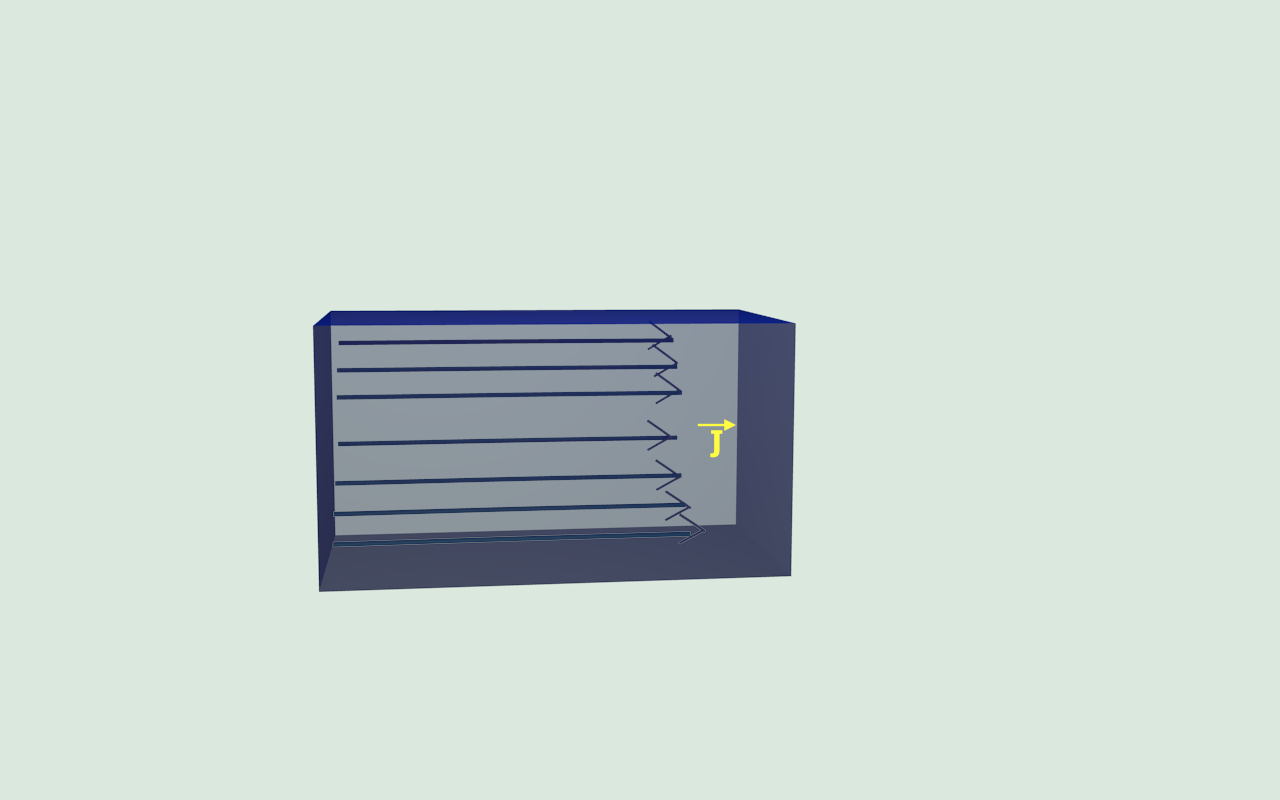
\includegraphics[height = 7cm, keepaspectratio]{graphes/blender_cuve_champvec.png}
%		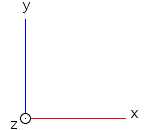
\includegraphics[height = 2cm, keepaspectratio]{graphes/axes.png}
		\caption{liquide faiblement ionisé soumis à un champ électrique $\vec{E}$, Blender}
		%		\end{subfigure}
	\end{center}
\end{figure}
\newline
On place un aimant de telle manière à générer un champ magnétique plus important sur une moitié du cube que l'autre.
\begin{figure}[!h]
	\begin{center}
	\centering
		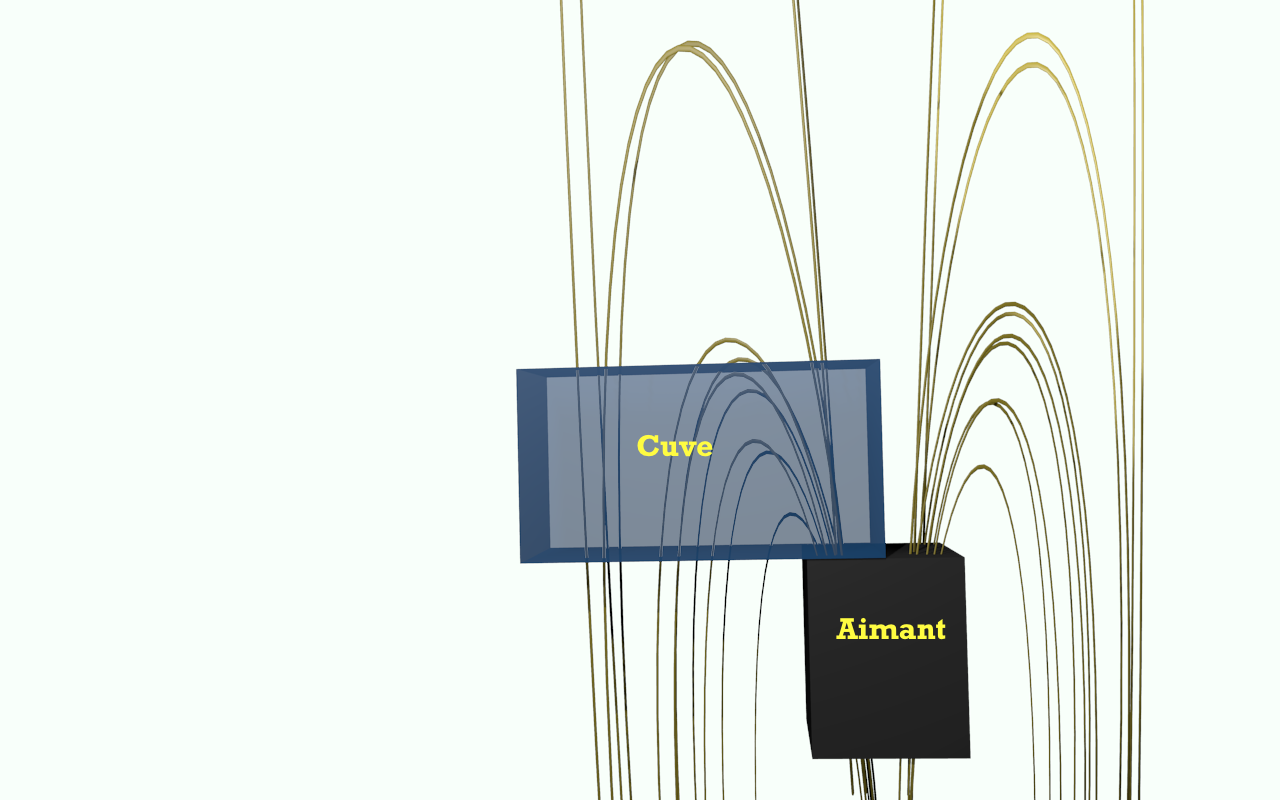
\includegraphics[height = 8cm, keepaspectratio]{graphes/blender_cuve_mag2.png} 
		%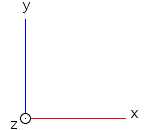
\includegraphics[height = 2cm, keepaspectratio]{graphes/axes.png}
		\caption{lignes de champ magnétique, Blender}
	\end{center}
\end{figure}
\newpage
La force magnétique $\vec{f_l}=\vec{j_0}\land\vec{B}$ permet ainsi de générer un tourbillon.\newline
\begin{figure}[h]
	\begin{center}
	\centering	
%	\begin{subfigure}[b]{0.3\textwidth}
%		\end{subfigure}
%		\begin{subfigure}[b]{0.3\textwidth}
		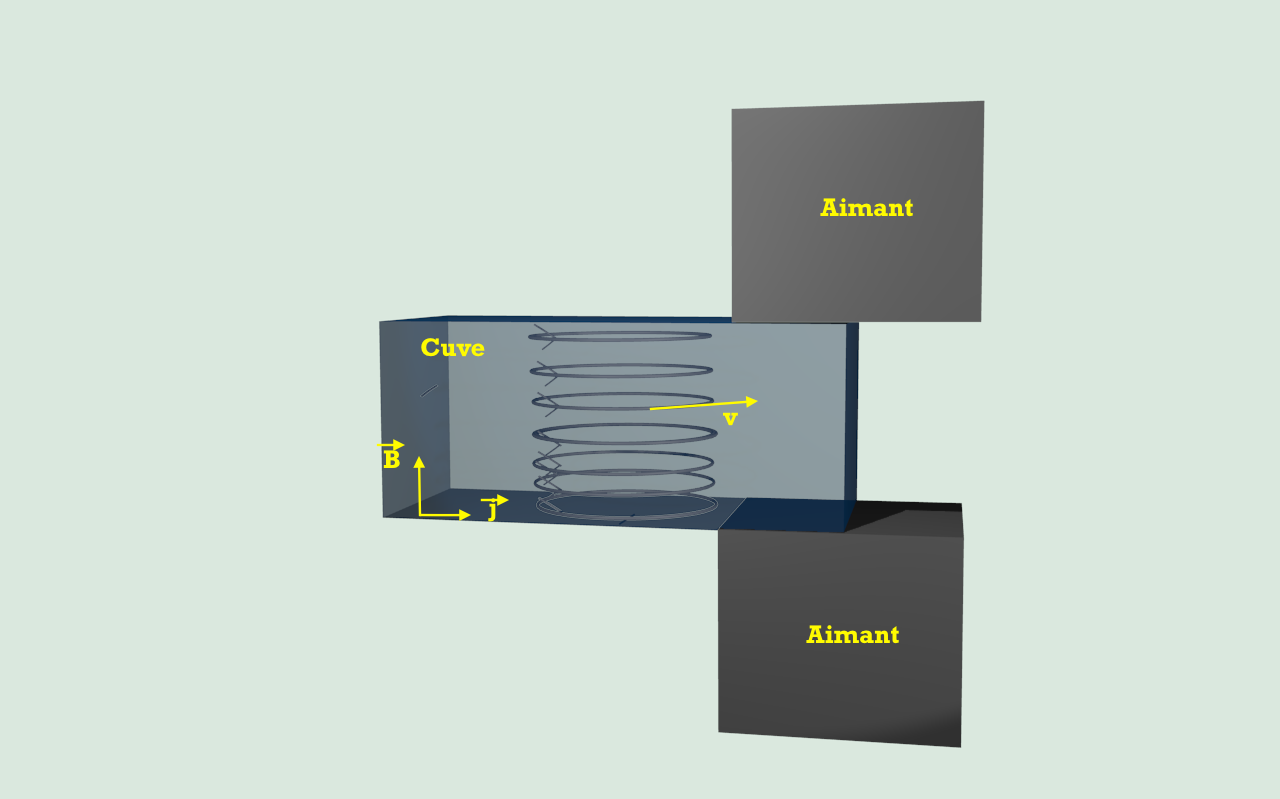
\includegraphics[height = 8cm, keepaspectratio]{graphes/champvec2.png}
%		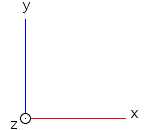
\includegraphics[height = 2cm, keepaspectratio]{graphes/axes.png}
		\caption{liquide faiblement ionisé soumis à un champ électrique et un champ magnétique $\vec{B}$, Blender}
%		\end{subfigure}
	\end{center}
\end{figure}
Afin de générer un tourbillon, on place deux aimants l'un en face de l’autre sur le deuxième tiers du parallélépipède pour créer un champ B~ vertical sur le tiers au milieu.
On place aussi deux électrodes sur les faces opposées du parallélépipède pour créer un courant uniforme de densité $\vec{j}$.
Une force de Laplace est générée sur une partie du fluide, due à la densité de courant en présence d’un champ magnétique $\vec{B}$, ce qui génère un tourbillon. \\
\begin{figure}[!h]
	\begin{center}
	\centering
		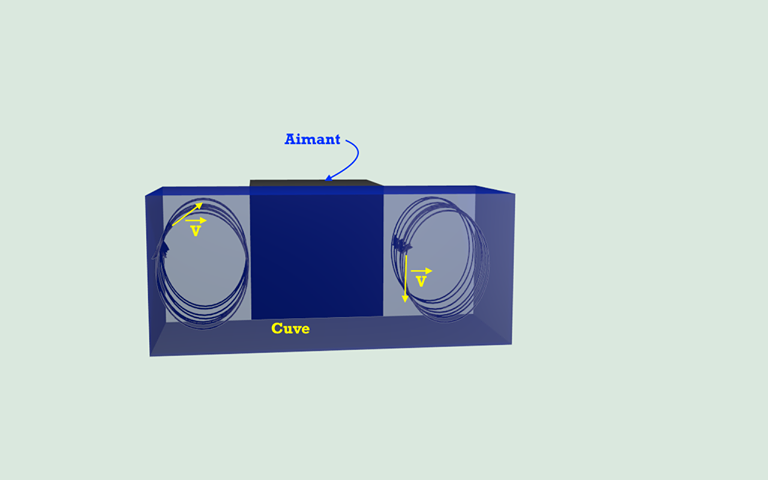
\includegraphics[height = 8cm, keepaspectratio]{graphes/config_centre.png} 
		%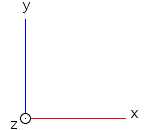
\includegraphics[height = 2cm, keepaspectratio]{graphes/axes.png}
		\caption{configuration avec 2 tourbillons pour un aimant, Blender}
	\end{center}
\end{figure}
On ajoute ensuite un autre aimant centré sur la cuve qui va lui induire des forces de Laplace de part et d'autres du parallélépipède de telle manière à générer deux tourbillons symétriques.\\
Puis en sommant les configurations, on arrive à un dispositif expérimental à trois tourbillons. \\
\begin{figure}[!h]
	\begin{center}
	\centering
		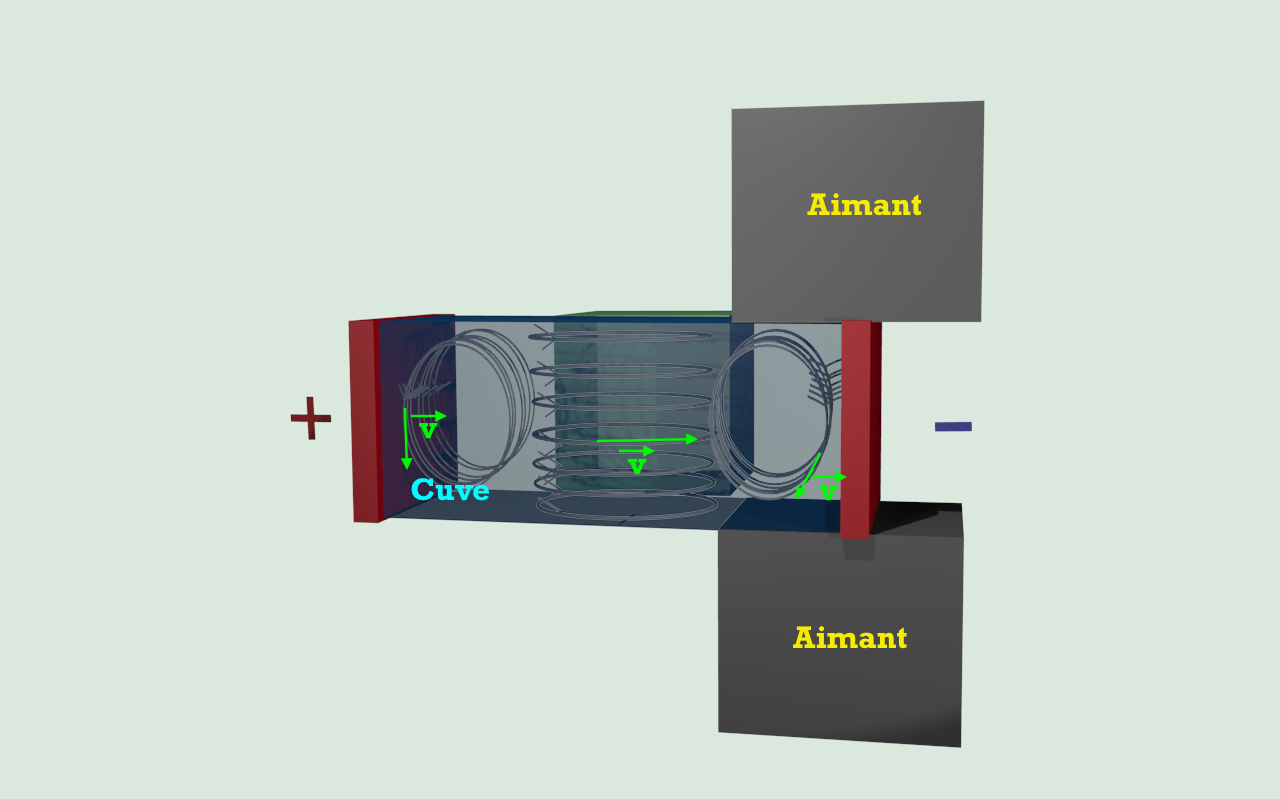
\includegraphics[height = 8cm, keepaspectratio]{graphes/blender_cuve_champvec3.png} 
		%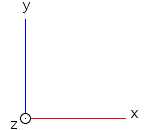
\includegraphics[height = 2cm, keepaspectratio]{graphes/axes.png}
		\caption{dispositif expérimental, Blender}
	\end{center}
\end{figure}
\\
\newpage
\newpage
\subsection{hypothèses de modélisation}
Nous devons d'abord modéliser notre système , car dans les cas de système faisant intervenir des équations à dérivées partielles , la bonne définition du système est primordiale, avec notamment les conditions aux limites.\\
Notre système \{fluide\} sera modélisé par un fluide à faible nombre de Reynolds (visqueux) incompressible régi par les équations de Stokes que nous poserons dans le chapitre suivant. La densité de courant $\vec{j_0}$ est supposé uniforme sur le fluide.


%=====================================================================================================================================
%												CHAPITRE 1 CALCUL DU CHAMP MAGNETIQUE
%==========================================================================================================================================================
\newpage
\chapter{Modélisation du champ Magnétique de l'aimant}

Nous allons nous intéresser en premier lieu à modéliser le champ magnétique d'un aimant pour pouvoir obtenir à terme les forces de Laplace s'exerçant sur le fluide pour caractériser l'écoulement.

Nous cherche ainsi à modéliser le champ d'induction magnétique $\vec{B}(x,y,z)$ induit par un aimant (Figure 1). L'objectif sera d'abord de déterminer le champ magnétique dans une configuration quelconque, pour ensuite exploiter ces résultats et les employer dans la résolution numérique de Navier Stokes. \\
\begin{figure}[h]
\begin{center}
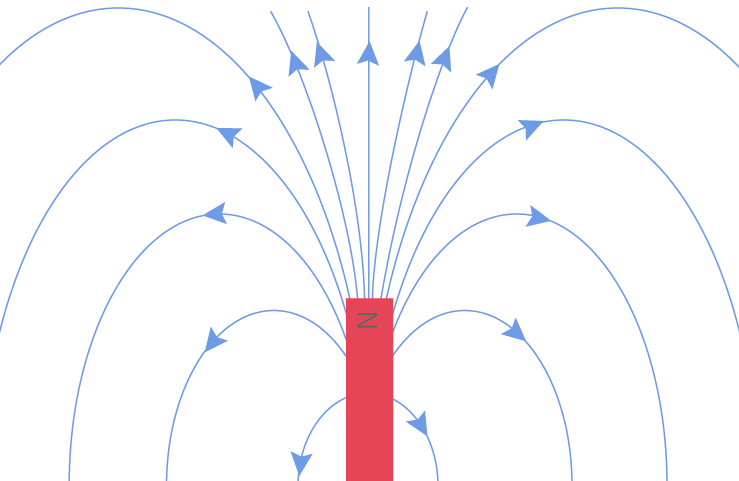
\includegraphics[height =4 cm, keepaspectratio]{graphes/champ_aimant1.png} %on affiche figure aimant
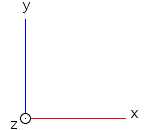
\includegraphics[height = 2cm, keepaspectratio]{graphes/axes.png}
\caption{champ magnétique d'un aimant coupe 2D}
\label{figure 1}
\end{center}
\end{figure}

On suppose que l'aimant à une longueur suffisante selon $\vec{z}$ pour être considéré comme infini selon l'axe $\vec{z}$.
On en déduit donc par le principe de Curie que le champ magnétique est invariant par translation selon $\vec{z}$. 
Ainsi \[\vec{B}(x,y,z) = \vec{B}(x,y)\]

On modélise donc le champ magnétique en deux-dimensions dans cette partie, dans la suite nous considérerons que le champ d'induction aura la même valeur selon la troisième dimension.
%======================= Mise en forme du probleme ================================================== 
\section{Mise en forme du problème}

Nous allons rechercher une solution du champ magnétique dans le domaine de résolution $\Omega$ (figure 2), $\Omega \subset R^{2}$. \\
\begin{figure}[h]
\begin{center}
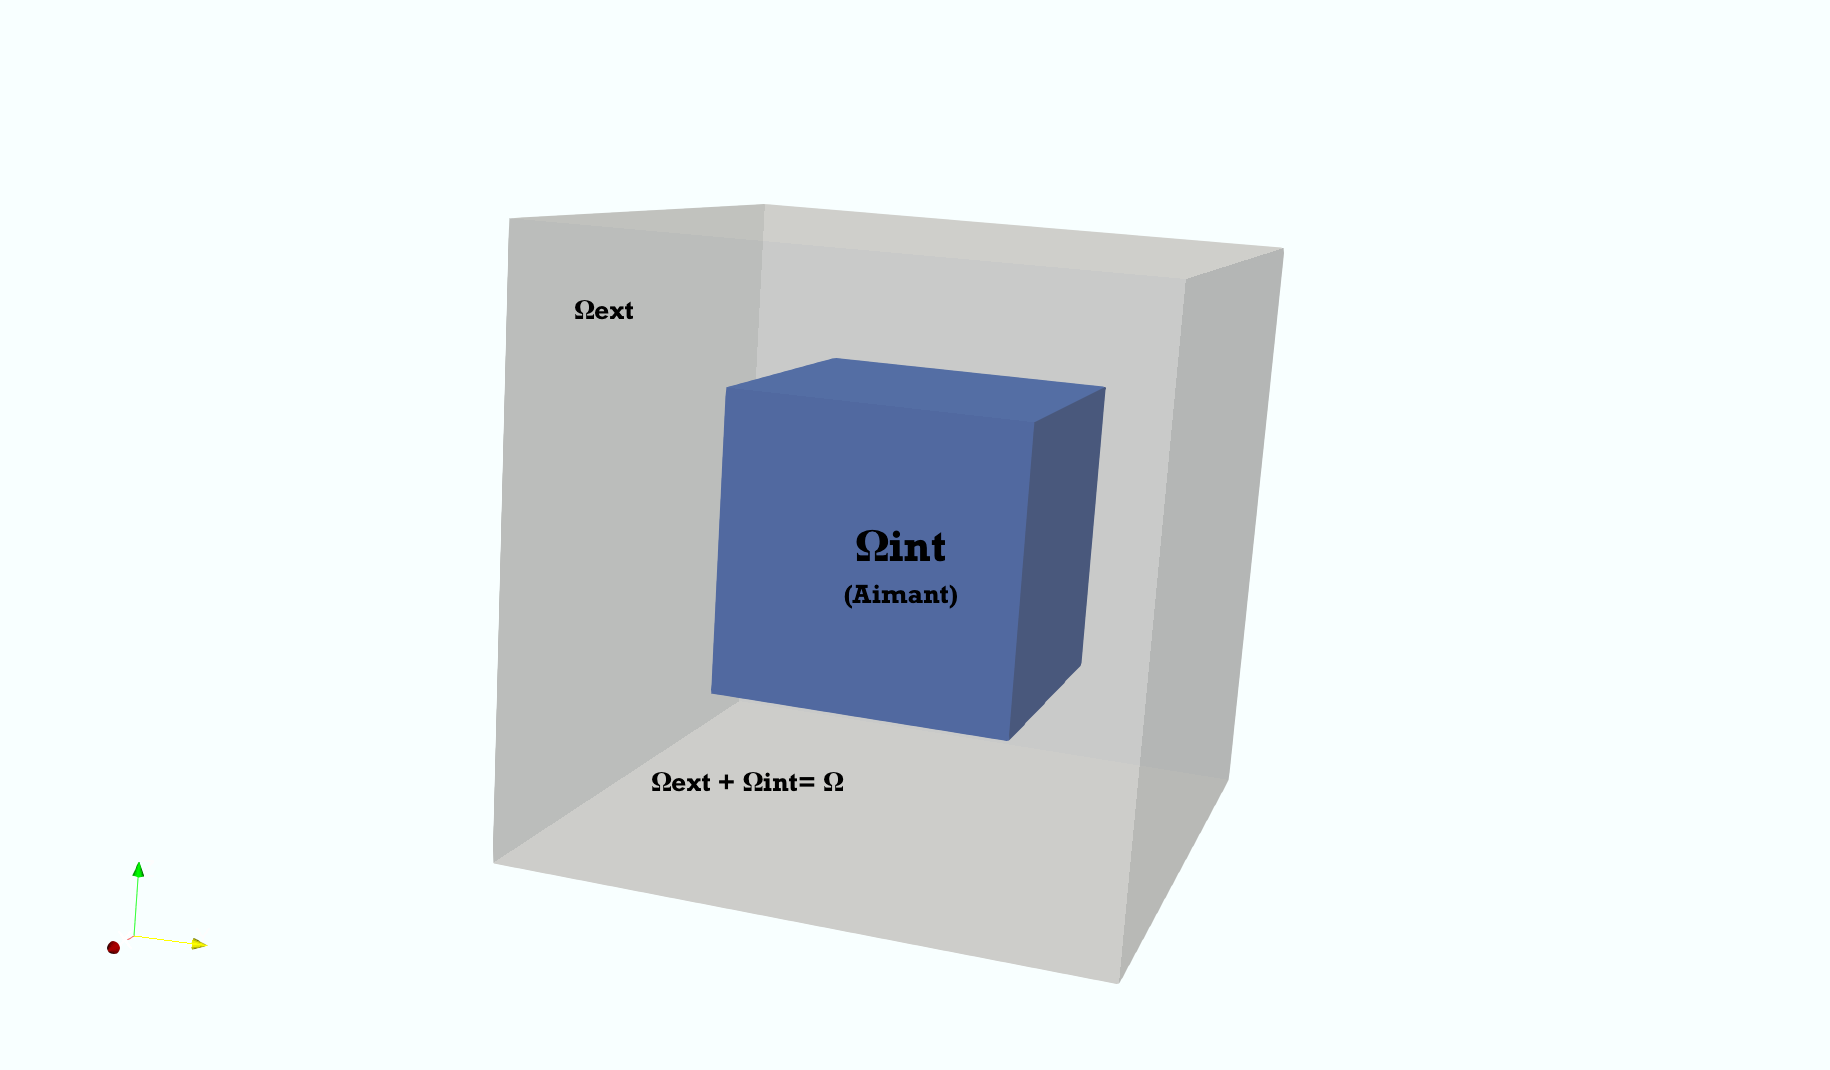
\includegraphics[height = 8cm, keepaspectratio]{graphes/Espacedetravail.png} 
\caption{domaines de résolution du problème, Blender}
\label{figure 2}
\end{center}
\end{figure}
On définit $\Omega_{int}$ le domaine de l'aimant, et $\Omega_{e}$ le domaine extérieur à l'aimant. 
\[\Omega_{e} = \Omega_{int} - \Omega\]

\newpage
On se place dans le régime stationnaire comme il n'y a pas de mouvements de l'aimant. \\
Le champ d'induction magnétique $\vec{B}$ est la somme du champs magnétique $\vec{H}$.

\[\vec{B}=\mu _{0}(\vec{H}+\vec{M})\]
$\mu _{0}$ est la perméabilité magnétique du vide. \\
L'aimantation $\vec{M}$ est nulle en dehors de l'aimant.
 
\[ 
\left\{
\begin{array}{ccc}
\begin{aligned}
	\vec{M} &= \vec{0} \  \text{dans} \ \Omega_{e} \\ 
	\vec{M} &= \vec{M_{0}} = \text{constante}  \ \text{dans}  \  \Omega_{\text{int}}
\end{aligned}
\end{array}
\right.
\]

Pour trouver le champ magnétique, on appliquer les équations fondamentales de la magnétostatique. L'équation de Maxwell nous donne 
\[
	\left\{
	\begin{array}{ccc}
	\begin{aligned}
		\Rot{\vec{H}} &= \vec {0} \\
		\Div{\vec{B}} &= 0
	\end{aligned}
	\end{array}
	\right.
\]

Le domaine étant simplement connexe, $\vec{H}$ dérive d'un potentiel $u$	.
\[
	\left\{
	\begin{array}{ccc}		
	\begin{aligned}
		\vec{H} &= \Grad{\vec{u}} \\
		\vec{B} &= \mu_{0}\times(\vec{\Grad{u}}+\vec{M})
	\end{aligned}
	\end{array}
	\right.
\]

Au sens des distributions pour toute fonction $\varphi\ $  dans $D(\Omega)$	
\[<\Div\vec{B},\varphi> \ = \ <-\vec{B},\vec{\Grad{\varphi}}>\]
On suppose $\vec{B} \in L^{3}_{1}(\Omega)$
\[<\Div\vec{B},\varphi> \ = \  -\int_{\Omega}\vec{B}. \vec{\Grad{\varphi}}\]
\[<\Div\vec{B},\varphi> \ = \ -\int_{\Omega}\mu_{0}(\vec{\Grad{u}}+\vec{M}) .{\Grad{\varphi}} = 0\]
Ainsi
\[\int_{\Omega}(\vec{\Grad{u}}+\vec{M}) . \vec{\Grad{\varphi}} = 0\]
Et comme $\vec{M}$ est nul en dehors du domaine $\Omega_{\text{int}}$ de l'aimant, on obtient (1)

On reconnait un problème de Dirichlet homogène qui admet une unique solution dans $H_{0}^{1}(\Omega)$ d'après le théorème de Lax-Migram.
\begin{equation}
\label{E}
\forall \varphi\ \in \Omega, \ \int_{\Omega}\bigtriangledown u .\bigtriangledown{\varphi} = -\vec{M_{0}}. \int_{\Omega_{int}}\bigtriangledown\varphi
\end{equation}

Adimensionnons (1)				:
\[
	\forall \varphi\  \in \Omega,\  \frac{1}{|\vec{M}_{0}|}\int_{\Omega}\bigtriangledown u.\bigtriangledown \varphi
	= -\vec{e}_{y}.\int_{\Omega_{int}}\bigtriangledown \varphi
\]
On prend pour la suite \[U =  \frac{u}{|\vec{M}_{0}|}  \] ce qui nous donne \[\vec{H^*} =\frac{\vec{H}}{M_0} \]
On établit ainsi \label{A}

\begin{equation}
\boxed{
\label{A}
	\forall \varphi\  \in \Omega,\ \int_{\Omega}\bigtriangledown U.\bigtriangledown \varphi
	=- \vec{e}_{y}.\int_{\Omega_{int}}\bigtriangledown \varphi}
\end{equation}
\\

\section{Méthode des éléments finis}

\subsection{Le maillage}
On recherche une solution approchée de l'équation numériquement en passant de l'espace continu à un espace discret. \\
\\
On utilise la méthode des éléments finis en recherchant une solution dans l'espace 
$V_{h} = \{u \ | \ u \in P^{1}(\Omega^{2}), u \in H^{1}_{0}(R^{2})\}$. \\
\\
On introduit une triangulation $T_{h}$ en subdivisant $\overline{\Omega}$, de bord $\Gamma \ = \ \partial\Omega$. 
Cette triangulation vérifie les propriétés suivantes :
\\
\begin{itemize}
  \item l’intersection de deux triangles K de $T_{h}$ doit être réduite à un sommet commun,\\ à une arête commune et entière ou à l'ensemble vide
  \item l’aire des triangles ne doit pas être nulle
  \item tous les coins du bord $\Gamma$ sont des sommets de triangles K de $T_{h}$
\end{itemize}

Le maillage ainsi construit est tel que
\[
\overline{\Omega} \ = \ \bigcup_{K \in T_{h}} K 
\]
\begin{figure}[h]
\begin{center}
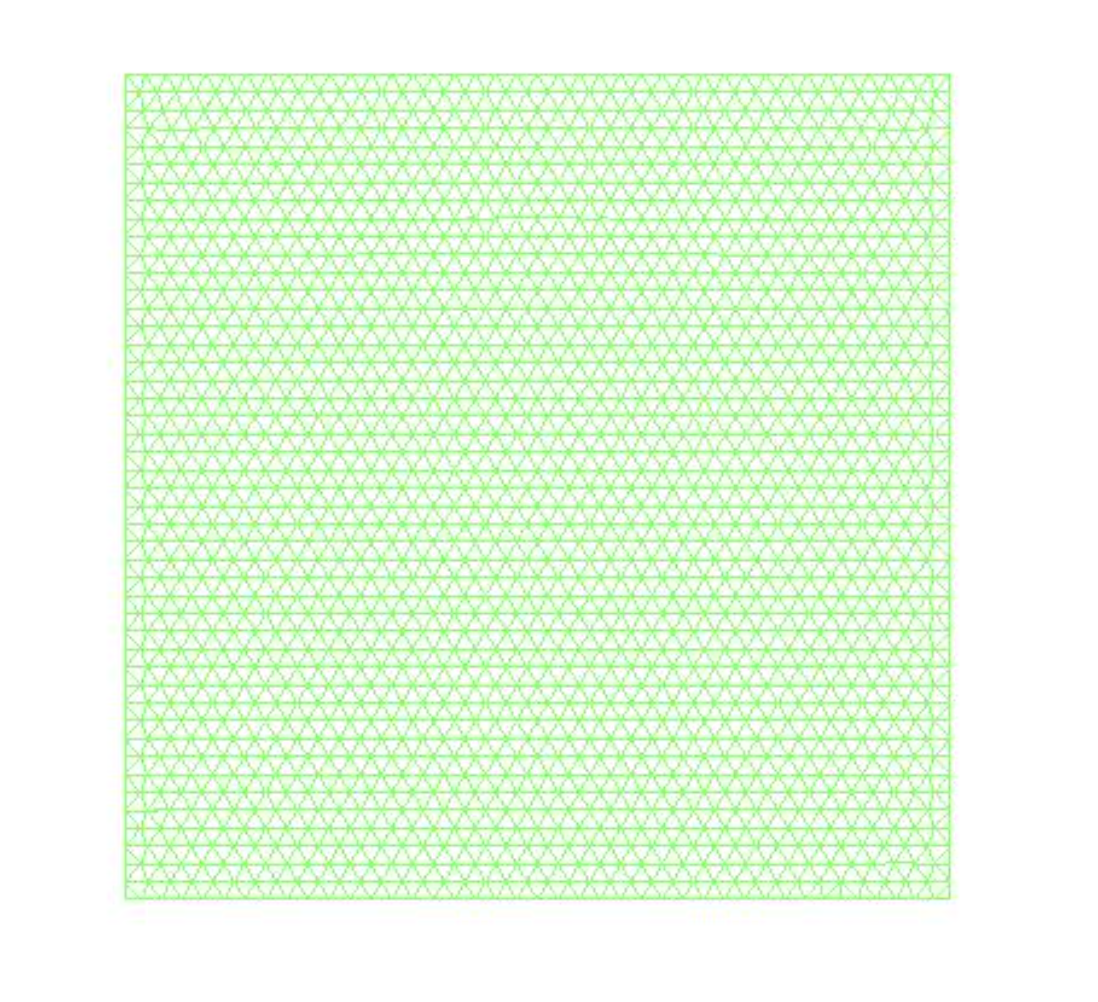
\includegraphics[height = 8cm, keepaspectratio]{graphes/Maillage_initial.png} 
\caption{\label{figure 3 } maillage effectué sur matlab à l'aide de mesh2D d'un carré 1$\times$1.05 avec un pas constant h = 0.1}
\end{center}
\end{figure}

On note que le maillage est caractérisé par la longueur de la plus petite arrête $h_{min}$ telle que 
\[
h_{min} \ = \ \min_{K \in T_{h}} h_{K}
\]
$h_{min}$ va notamment déterminer l'erreur entre la solution continue et la solution discrète.
On choisit une base de $V_{h}$, on prend la famille des fonctions de base  \\ $\varphi_{1}, \varphi_{2}, ..., \varphi_{N_{h}}$  telles qu'elles valent 1 en un sommet d’un triangle, et 0 pour tous les autres sommets. On note $P_{1},P_{2}, ..., P_{N_{h}}$ les sommets des triangles du maillage.
Les fonctions de base sont donc définies ainsi :
\[
\forall i,j \in [1, N_{h}]^{2} \ \varphi_{i} \in L^{2}(\Omega),\ \varphi_{i}(P_{j}) \ = \ \delta_{ij} \ \
\varphi_{i} \ = \ 0 \ sur \ \Gamma \]
Le support de $ \varphi_{i}$ est la réunion de tous les triangles ayant pour sommet $P_{i}$.\\
On vérifie que la famille ($\varphi_{1}, \varphi_{2}, ..., \varphi_{N_{h}}$) est une base de $V_{h}$.
Ainsi toute fonction g dans $V_{h}$ peut s'écrire comme une combinaisons linéaire des $\varphi_{i}$
\[
g = \sum_{i=1}^{N_{h}}{\ g_{i}\varphi_{i}} \text{ \ \ où } g_{i} = g(P_{i}),\  i= 1,2,...,N_{h}
\]

%=====================================================================================================
\subsection{Mise en équation}
%=======================================================================================================

Réécrivons (1.2) dans $V_{h}$ : 

\[
	\forall \varphi \in V_{h} , \ \int_{\Omega}\bigtriangledown u_{h}. \bigtriangledown \varphi = -\vec{M_{0}}. \int_{\Omega_{int}}\bigtriangledown \varphi
\]
Nous pouvons écrire $u_{h} = \sum_{i=1}^{N_{h}}{\ U_{i}\varphi_{i}} \text{ \ \ où } U_{i} = U(P_{i}),\  i= 1,2,...,N_{h}$ \\ et choisir $\varphi\ =\ \varphi_{i}$
ainsi
\[
	\int_{\Omega}\bigtriangledown u_{h}.\bigtriangledown \varphi\ 
	=\ 
	\sum_{i, j \in [1, N_{h}]^{2}} \int_{\Omega}u_{i}\bigtriangledown\varphi_{i}. \bigtriangledown\varphi_{j} 
	= 
	\sum_{i,j \in [1, N_{h}]^{2}} A_{ij} u_{i}
\]
avec A la matrice $N_{h} \times N_{h}$ de coefficients
\[
A_{ij}  = \int_{\Omega}\bigtriangledown\varphi_{i}.\bigtriangledown\varphi_{j}
\]
et si on introduit le vecteur $\vec{f}$ de composantes $f_{1},\ f_{2},..., f_{N_{h}}$ définies par
\[
f_{j} =  -\vec{e_{y}}.\int_{\Omega} \bigtriangledown\varphi_{j}
\]
Alors l'équation (2) revient de manière équivalente à résoudre le système linéaire 
\[
	A \times U =F
\]
 avec 
\[
U = 
\begin{pmatrix}
   u_{1} \\
   u_{2} \\
   \vdots \\
   u_{N_{h}}
\end{pmatrix}
\ \ F = 
\begin{pmatrix}
   f_{1} \\
   f_{2} \\
   \vdots \\
   f_{N_{h}}
\end{pmatrix}
\quad
A_{ij}  = \int_{\Omega}\bigtriangledown \varphi_{i}. \bigtriangledown \varphi_{j}
\]
On appelle A la matrice de rigidité.  \\

%================= passage element de reference =====================================================
\newpage
\subsection{Passage à un élément de référence}
Pour les calculer numériquement les matrices on utilise un triangle de référence normalisé $\hat{T}$. On passe du triangle $\Hat{T}$ à $T$ à l'aide de la transformation $F$. 
\begin{figure}[h!]
\begin{center}
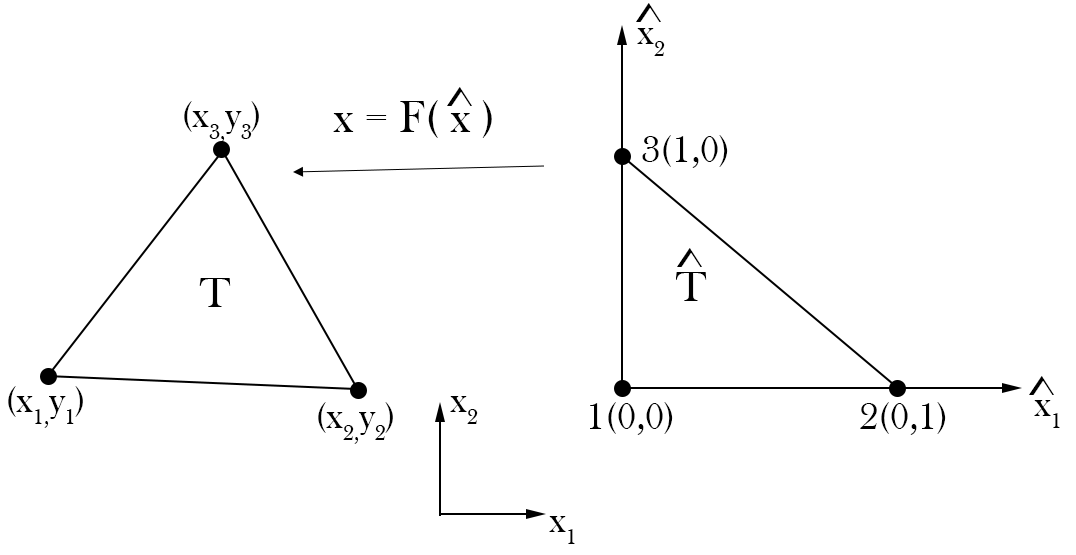
\includegraphics[height = 6cm, keepaspectratio]{graphes/transformation_de_maillage.png} 
\caption{\label{figure 4 } passage à un maillage de référence}
\end{center}
\end{figure}
On a pour le calcul du gradient de $\varphi_{i}$
\[ \bigtriangledown_{\hat{x}} \hat{\varphi} = (J)^{T} \bigtriangledown_{x} \varphi  \]
où J est la matrice Jacobienne de la transformation.
Calculons la matrice Jacobienne qui va dépendre des coordonnées $(x_{i},y_{i})$ des sommets pour chaque triangle.
\[
x = \begin{pmatrix}
   x_{1} \\
   x_{2} 
\end{pmatrix}
= \begin{pmatrix}
   F_{1}(\hat{x}) \\
   F_{2}(\hat{x}) 
\end{pmatrix}
= \begin{pmatrix}
   \hat{x}_{1} \\
   \hat{x}_{2} 
\end{pmatrix}
= J \times \hat{x} + C
\]
On obtient ainsi à l'aide d'un changement de variable le calcul de la matrice de rigidité (voir annexe A) : 
\[
\boxed{
\begin{aligned}
A_{ij} = 
	\iint_{\Omega}\bigtriangledown_{x}{\varphi_{i}} \bigtriangledown_{x}{\varphi_{j}} &= 
	\sum_{T \in \text{Supp}(\varphi_{i})\times \text{Supp}(\varphi_{j})}	
	\frac{\text{aire}(T)^{2}}{4}
	\begin{pmatrix}
   		y_{3}-y_{1} &  	x_{1}-x_{3}\\
   		y_{1}-y_{2} &  x_{2}-x_{1}
	\end{pmatrix}
	^{2}
	\bigtriangledown_{\hat{x}} \hat{\varphi_{i}}
	\bigtriangledown_{\hat{x}} \hat{\varphi_{j}}
\end{aligned}}
\]
\\
\\
Calculons à présent le terme source $f_{j} =  -\vec{e_{y}}.\int_{\Omega} \bigtriangledown\varphi_{j}$.
\\
\\
D'après Green-Ostrogradsky
\[
	\iint_{\Omega}\bigtriangledown_{x}{\varphi_{i}} =\ 
	\int_{\partial\Omega_{\text{int}}}\varphi_{i}.\vec{\text{n}} \ \partial s
\]

Ainsi	
\[
	\begin{aligned}
		\int_{\partial\Omega_{\text{int}}}\varphi_{i}.\vec{\text{n}}\ \partial s &= 
		\sum_{e \in \partial\Omega_{\text{int}}}\ \int_{e}\varphi_{i}.\vec{\text{n}}_{e}\ \partial s \\ &=  
		\sum_{e \in \partial\text{supp}(\varphi_{i})}\ \int_{e}\varphi_{i}.\vec{\text{n}}_{e}\ \partial s
	\end{aligned}
\]
où $\vec{\text{n}}_{e}$ est le vecteur unitaire normal sortant à l'arête e. \\
\begin{figure}[h]
\begin{center}
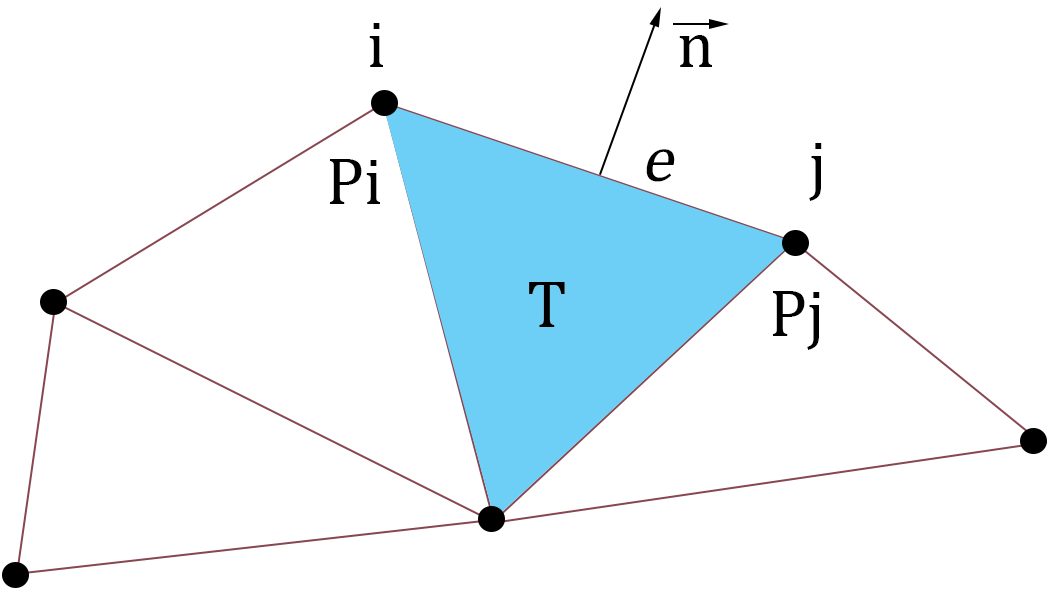
\includegraphics[height = 4cm, keepaspectratio]{graphes/bord.png}
\caption{arêtes}
\label{figure 1}
\end{center}
\end{figure}
\[
	|e|\times \vec{\text{n}}_{e}
	=
	\begin{pmatrix}
		y_{j}-y_{i} \\
		x_{i}-x_{j}
	\end{pmatrix}
\]
avec le changement de variable $x = s\times \text{Pi} + (1-s)\times \text{Pj}$,\ \ $s \in [0;1]$
\[
	\int_{e}\varphi_{i}.\vec{\text{n}}_{e}\ \partial s = |e|(\int_{0}^{1}\varphi_{i}\ \partial x ).\vec{\text{n}}_{e}
\]
avec 
\[
	\int_{0}^{1}\varphi_{i}\ \partial s  = \text{aire du triangle rectangle de coté |e| et de hauteur 1} = \frac{|e|}{2}
\]
d'où
\[
	\int_{e}\varphi_{i}.\vec{\text{n}}_{e}\ \partial s =
	|e|(\int_{0}^{1}\varphi_{i}\ \partial x ).\vec{\text{n}}_{e} =
	\frac{|e|}{2}.\vec{\text{n}}_{e} = 
	\frac{|e|^{2}}{2}
	\begin{pmatrix}
		y_{2}-y_{1} \\
		x_{1}-x_{2}
	\end{pmatrix}	
\] 
Au final
\[
	\iint_{\Omega}\bigtriangledown_{x}{\varphi_{i}} =
	\sum_{e \in \partial \text{supp}(\varphi_{i})}\ \int_{e}\varphi_{i}.\vec{\text{n}}_{e}\ \partial s =
	\sum_{e \in \partial\text{supp}(\varphi_{i})}
	\frac{|e|}{2}
	\begin{pmatrix}
		y_{2}-y_{1} \\
		x_{1}-x_{2}
	\end{pmatrix}
\]
\[
	\iint_{\Omega}\bigtriangledown_{x}{\varphi_{i}} =
	\sum_{e \in \partial \text{supp}(\varphi_{i})}
	\frac{|e|}{2}
	\begin{pmatrix}
		x_{2}-x_{1} \\
		y_{1}-y_{2}
	\end{pmatrix}
\]
Au final 
\[\boxed{f_{j} =  -\vec{e_{y}}.\sum_{e \in \partial \text{supp}(\varphi_{i})}
	\frac{|e|}{2}
	\begin{pmatrix}
		x_{2}-x_{1} \\
		y_{1}-y_{2}
	\end{pmatrix}}
\]

				

%====================== Calcul du gradient =========================================================							
\subsection{Calcul du Gradient}

Les calculs précédents nous permettent de trouver après résolution le potentielle $u$, ce que nous voulons obtenir à l'issue de notre étude est le champ d'induction magnétique $\vec{B}$ que l'on trouve par $\vec{B}= \bigtriangledown u$.
\\
\newline  On écrit la forme variationnelle dans $V_{h}$ (ainsi $\vec{B}$ suit une décomposition dans $V_h$, tel que $\vec{B}=\sum_{i} B_{xi}\varphi_i:$

\[
\begin{aligned}
		\forall \varphi \in V_{h} , \ \int_{\Omega}B.  \varphi &= \int_{\Omega}\bigtriangledown u.\varphi  \\
		\sum_{i,j}\;  \sum_{T \in \text{Supp}(\varphi_{i})\times \text{Supp}(\varphi_{j})}B_{i}\int_{T} \varphi_i\varphi_j & =  \sum_{i}  \sum_{T \in \text{Supp}(\varphi_{i})\times \text{Supp}(\varphi_{j})} u_i \int_{T}\bigtriangledown\varphi_i\varphi_j  
\end{aligned}
\]
Nous pouvons écrire l'équation ci dessus sous forme matricielle, en introduisant les matrices M et C, définit de la façon suivante :
\[
		M_{ij}=\int_{T} \varphi_i.\varphi_j \ \text{appellé la matrice de masse}
\]
\[
		C_{ij}=\int_{T} \bigtriangledown\varphi_i.\varphi_j 
\]
L'équation devient ainsi un problème linéaire sous forme matricielle  
\[
	M \times B=C \times U
\] 

Soit 
\[
	\boxed{B =M\up{-1}\times C \times U}
\]
Calculons ainsi les termes de la matrice C:
\[
\begin{aligned}
C_{ij} &= \iint_{\Omega}\bigtriangledown\varphi_i\varphi_j dx      
       = \sum_{K\in supp\varphi_j}\bigtriangledown_K\varphi_i \iint_{K} \varphi_jdx \\
	 &= \sum_{K\in supp\varphi_j}(J\up{-1}_K)^{T}(\bigtriangledown_{\hat{K}} \hat{\varphi_i})\iint_{\hat{K}}  |J_{K}| \hat{\varphi_j}\hat{dx} \\
	&= \sum_{K\in supp\varphi_j}(J\up{-1}_K)^{T}|J_K| (\bigtriangledown_{\hat{K} }\hat{\varphi_i})\iint_{\hat{K}}  \hat{\varphi_j}\hat{dx}
\end{aligned}
\]
\[\boxed{C_{ij} =  \sum_{K\in supp\varphi_j}(J\up{-1}_K)^{T}|J_K| (\bigtriangledown_{\hat{K} }\hat{\varphi_i})\iint_{\hat{K}}  \hat{\varphi_j}\hat{dx}} \]

Nous allons calculer pour l'implémentation algorithmique des matrice élémentaires qui vont regrouper sur chaque triangle les contributions croisés des trois nœuds, soit neuf termes dans chaque matrice élémentaire.
\newline
Calculons une matrice élémentaire de C sur un triangle K du maillage qui aura donc pour composantes (si on se place selon la composante x du gradient ) 

\[
|J_K| \times
\begin{pmatrix}
   	\bigtriangledown_{\hat{K} }{\varphi_1}_{|x}\iint_{\hat{K}}  \hat{\varphi_1}&\bigtriangledown_{K}{\varphi_1}_{|x}\iint_{\hat{K} } \hat{\varphi_2} &\bigtriangledown_{K}{\varphi_1}_{|x}\iint_{\hat{K} } \hat{\varphi_3}\\ 
  \bigtriangledown_{K }{\varphi_2}_{|x}\iint_{\hat{K }} \hat{\varphi_1} & \bigtriangledown_{K }{\varphi_2}_{|x}\iint_{\hat{K} }\hat{\varphi_2} & \bigtriangledown_{K }{\varphi_2}_{|x}\iint_	{\hat{K} } \hat{\varphi_3} \\
  \bigtriangledown_{K }{\varphi_3}_{|x}\iint_{\hat{K} } \hat{\varphi_1}&\bigtriangledown_{K }{\varphi_3}_{|x}\iint_{\hat{K} } \hat{\varphi_2} & \bigtriangledown_{K}{\varphi_3}_{|x}\iint_{\hat{K} } \hat{\varphi_3}
\end{pmatrix} 
\]
Calculons les intégrales :


\[	
  \left\{
    \begin{aligned}
      \iint_{\hat{K}} \hat{\varphi_1}{\hat{dx}} &= \int_{0}^{1}\int_{0}^{1-{\hat{x}}_2} (1-{{\hat{x}}_1}-{{\hat{x}}_2}) \hat{dx}_1 \hat{dx}_2 &=1/6\\
      \iint_{\hat{K} } \hat{\varphi_2}\hat{dx} &= \int_{0}^{1}\int_{0}^{1-{\hat{x}}_2} {{\hat{x}}_1} \hat{dx}_1 \hat{dx}_2 =1/6\\
       \iint_{\hat{K} } \hat{\varphi_3}\hat{dx} &= \int_{0}^{1}\int_{0}^{1-{\hat{x}}_2} {{\hat{x}}_1} \hat{dx}_1 \hat{dx}_2 =1/6\\
    \end{aligned}
  \right.
\]
\newpage
On a ainsi a matrice élémentaire du terme C sur un triangle K:

\[
\frac{1}{6}\times
	\begin{pmatrix}
   		\bigtriangledown_{K}{\varphi_1}_{|x} & \bigtriangledown_{K}{\varphi_1}_{|x} &  										    
   		\bigtriangledown_{K} {\varphi_1}_{|x} \\ 
    	\bigtriangledown_{K }{\varphi_2}_{|x} & \bigtriangledown_{K }{\varphi_2}_{|x} &  
    	\bigtriangledown_{K }{\varphi_2}_{|x} \\    										        
    	\bigtriangledown_{K}{\varphi_3}_{|x} & \bigtriangledown_{K}{\varphi_3}_{|x} & \bigtriangledown_{K}{\varphi_3}_{|x} \\ 
    \end{pmatrix} 
\]
\newline
Calculons également directement les matrices élémentaires pour la matrice de masse M définis par :
\[
M_{ij}=\iint_\Omega \varphi_i \varphi_j
\]
Sur un triangle K du maillage , on obtient de la même manière que précédemment 
\[
  \left.
    \begin{aligned}
		M_{ij}\up{K}=\int_0^{1}\int_0^{1-{\hat{x}}_2}|J_K|\hat{\varphi_i}(\hat{x})\hat{\varphi_j}(\hat{x})d\hat{x}\\
		=2\times\text{aire}(K)\times\int_0^{1-{\hat{x}}_2}\hat{\varphi_i}(\hat{x})\hat{\varphi_j}(\hat{x})d\hat{x}
    \end{aligned}
  \right.
\]
Il suffit donc de calculer les intégrales 
\[
	\int _0^{1}\int_0^{1-{\hat{x}}_2}\hat{\varphi_i}(\hat{x})\hat{\varphi_j}(\hat{x})d\hat{x}
\]
\\
par symétrie 
\[
	\forall i \int _0^{1}\int_0^{1-\hat{x}_{2}}\hat{\varphi_i}\up{2}= \int _0^{1} \int_0^{1-\hat{x}_{2}}\hat{x}_{2}^{2}d\hat{x}_{1}d\hat{x}_{2}=\frac{1}{12}
\]
\\%
\[
	\forall i \neq j \int _0^{1}\int_0^{1-{\hat{x}}_2}\hat{\varphi_i} \times \hat{\varphi_j}=\int _0^{1} \int_0^{1-\hat{x}_{2}}\hat{x}_{1}\hat{x}_{2}d\hat{x}_{1}d\hat{x}_{2}=\frac{1}{24}
\]
\\%
On en déduit la matrice de masse élémentaire sur un triangle de maillage 
\\%
\[
	\boxed{M\up{K}=\frac{\text{aire}(K)}{12}\times 
	\begin{pmatrix}
   		2 & 1 & 1 \\
   		1 &  2 & 1 \\
   		1 &  1 & 2
	\end{pmatrix}}
\]

%====================== Algorithme Matlab ======================================================= 
\subsection{Implémentation algorithmique}

Pour la résolution du problème nous utiliserons matlab avec la bibliothèque Mesh2D par Darren Engwirda pour la création du maillage 2D.
La résolution est effectué sur un maillage $5\times 5$ avec en son centre un aimant de taille $1\times 1$.

\begin{figure}[h]
	\begin{center}
	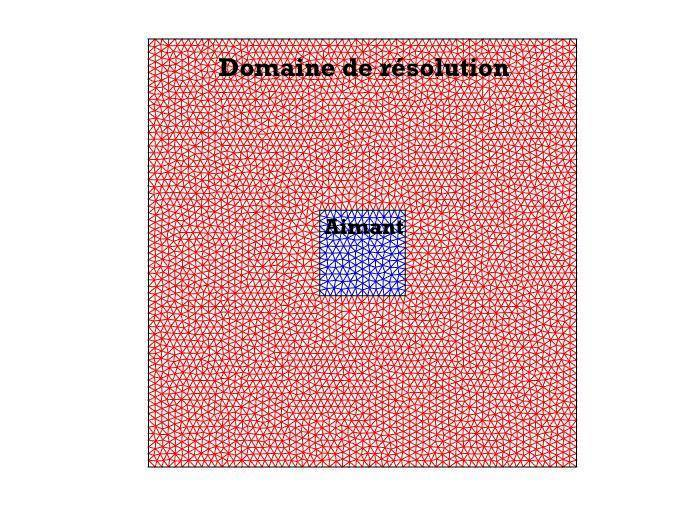
\includegraphics[height = 7cm, keepaspectratio]{graphes/maillage_resolution_champ_magnetique.jpg} 
	\caption{\label{figure 3 } maillage effectué sur matlab à l'aide de mesh2D dans la configuration décrite pour un pas h = 0.1}
	\end{center}
\end{figure}

Pour le calcul nécessaire des différentes matrices afin de résoudre le problème linéaire $A\times U = F$, les algorithmes reposent sur la même méthodologie de calcul :
Par exemple pour le calcul de la matrice A : 
\[
\begin{aligned}
A_{ij} = 
	\iint_{\Omega}\bigtriangledown_{x}{\varphi_{i}} \bigtriangledown_{x}{\varphi_{j}} &= 
	\sum_{T \in \text{Supp}(\varphi_{i})\times \text{Supp}(\varphi_{j})}	
	\frac{\text{aire}(T)^{2}}{4}
	\begin{pmatrix}
   		y_{3}-y_{1} &  	x_{1}-x_{3}\\
   		y_{1}-y_{2} &  x_{2}-x_{1}
	\end{pmatrix}
	^{2}
	\bigtriangledown_{\hat{x}} \hat{\varphi_{i}}
	\bigtriangledown_{\hat{x}} \hat{\varphi_{j}}
\end{aligned}
\]
Le principe consiste à ne pas rechercher le support croisé des fonctions $\varphi_i$ et $\varphi_j$ (ce qui donnerait une complexité trop importante) mais à boucler sur les triangles et placer dans la matrice les contributions correspondantes à chacun de leurs nœuds avec leur indices. Notamment avec l'outil matriciel $sparse$ de matlab qui permet d'exploiter en temps de calcul et d'espace mémoire le fait que la matrice de rigidité A est creuse, comme pour deux fonction $\varphi_{i}$ et $\varphi_{j}$ l'intersection de leurs support se réduit à deux triangles.
\\
\\
Ainsi pour le calcul de A chaque triangle engendre une matrice élémentaire $ 3\times 3$ (car 3 nœuds pour chaque triangle donc 9 termes croisés) symétrique vu le calcul du terme $A_{ij}$ dont on place les terme dans la matrice A à chaque itération sur les triangles.
\\
\\Le principe est le même pour le terme source, pour chaque triangle appartenant au bord de l'aimant avec comme noeuds sur le bord les nœuds $\text{p}_{i}$ et  $\text{p}_{j}$ on place deux fois le même terme $\frac{|e|}{2}\begin{pmatrix} 
   									0 & 1\\
								\end{pmatrix}^{T}.
								\vec{\text{n}}_{e}$ 
(que l'on à calculé p.21) aux indices $\text{p}_{i}$ et  $\text{p}_{j}$ dans la matrice du terme source.
\\
\\
Et de même également pour le calcul des matrices M et C pour le gradient, dont nous avons explicité les matrices élémentaires.	

Voici une présentation succinte de l'algorithme de résolution, les fonctions utilisés sont détaillé dans l'annexe \ref{annexe_2}.

Pour la génération du maillage, on utilise la fonction meshfaces fournis par la bibliothèque Mesh2D par Darren Engwirda
\begin{verbatim}
 [v,t,fnum] = meshfaces(node,edge,face,hdata); %construction du maillage
 
 v : vecteur colonne regroupant les coordonnées des nœuds
 t : table de connectivité des triangle
 fnum : numéros de face des triangles du maillages (1 ou 2), 
 si sur le domaine des l'aimant ou de la cuve
\end{verbatim}
Calcul de la matrice de rigidité A et de la matrice de masse M : 
\begin{verbatim}
[M, nn, ibint, ic2] = matrixP1final(v,t,fnum,node1,edge1,node2,edge2);
[A]= matrixP1vect(v,t);
\end{verbatim}

On enlève les noeuds sur le bord du domaine de résolution comme la condition aux limite impose que $\Delta u = 0$ sur le bord, que nous considerons équivalente à $u = 0$ 
\begin{verbatim}
A1 = A1(ic2,ic2);	%ic2 sont les noeuds intérieurs du maillage
sol = A1\M;			%résolution linéaire
\end{verbatim}
Calcul du gradient de $u$ :
\begin{verbatim}
B = gradient(u,v,t);
 quiver(X,Y,B_X,B_Y);		%affichage du résultat final
\end{verbatim}

%====================== resultats  ===========================================================================
 
\subsection{Résultats de la simulation}

Voici les résultats de la simulation pour un maillage de pas 0.2 et de taille $5 \times 5$ pour un aimant de taille $1 \times 1$
\begin{figure}[!h]
\begin{center}
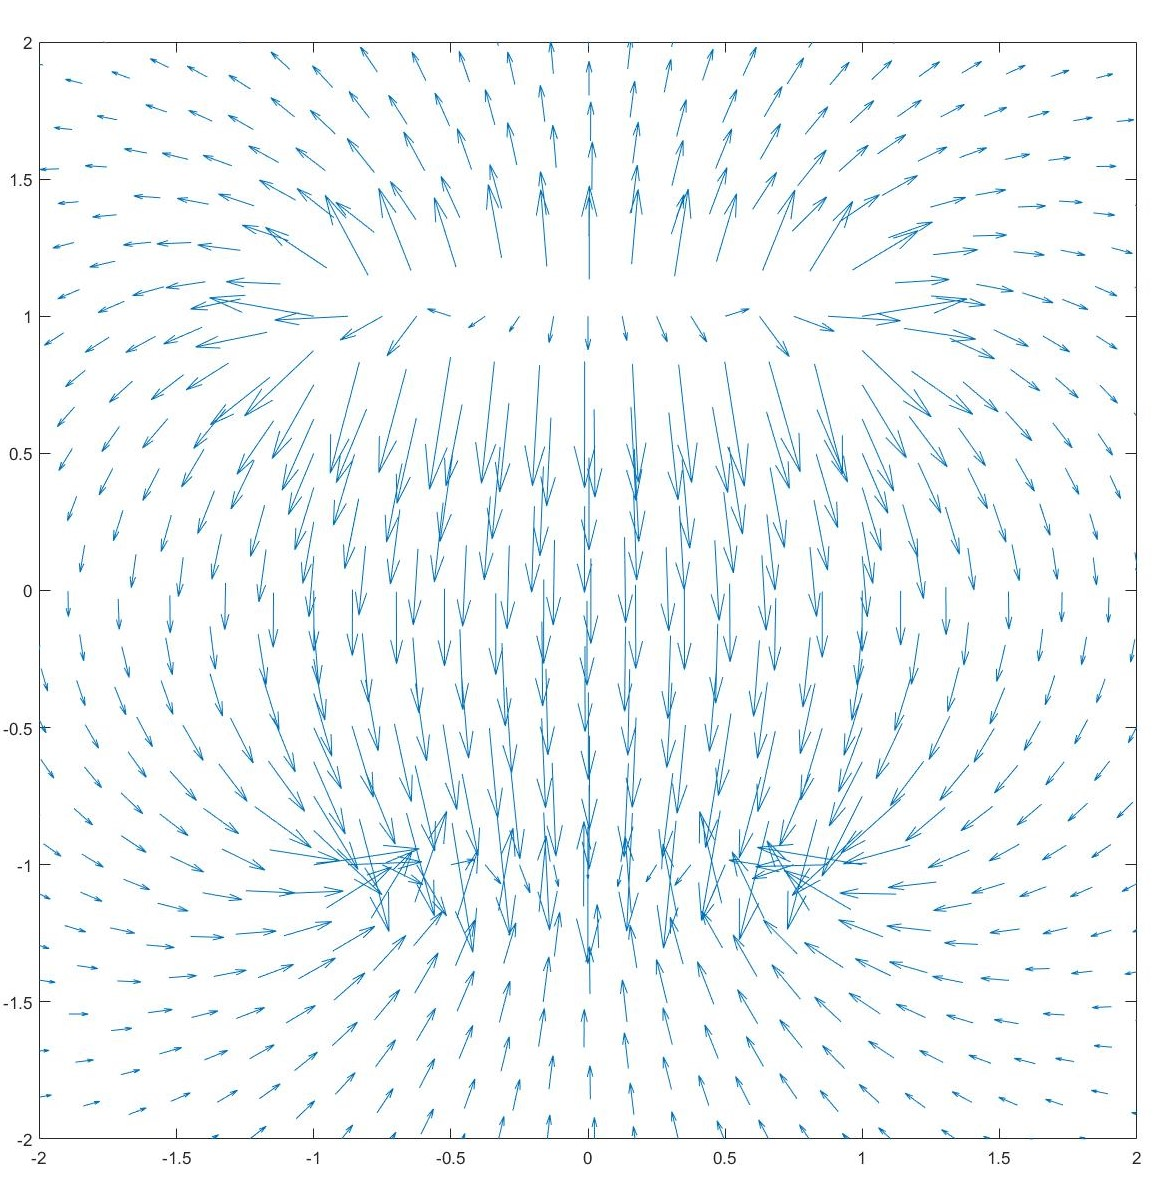
\includegraphics[height = 10cm, keepaspectratio]{graphes/resultat_champ.jpg}
\caption{affichage $quiver$ du champ magnétique, fenêtre centrée sur [-2, 2]}
\label{figure 1}
\end{center}
\end{figure}
On voit que les vecteurs suivent les trajectoires des lignes de champs que l'on peut attendre d'un aimant.
On peut s'inquiéter de la discontinuité des valeurs au bord de l'aimant mais ce la est en accord avec la formulation du champ d'induction comme la somme d'un champ d'excitation et d'une aimantation, nulle en dehors de l'aimant $\vec{B}=\mu _{0}(\vec{H}+\vec{M})$, d'où cette discontinuité que l'on observe.
\begin{figure}[!h]
\begin{center}
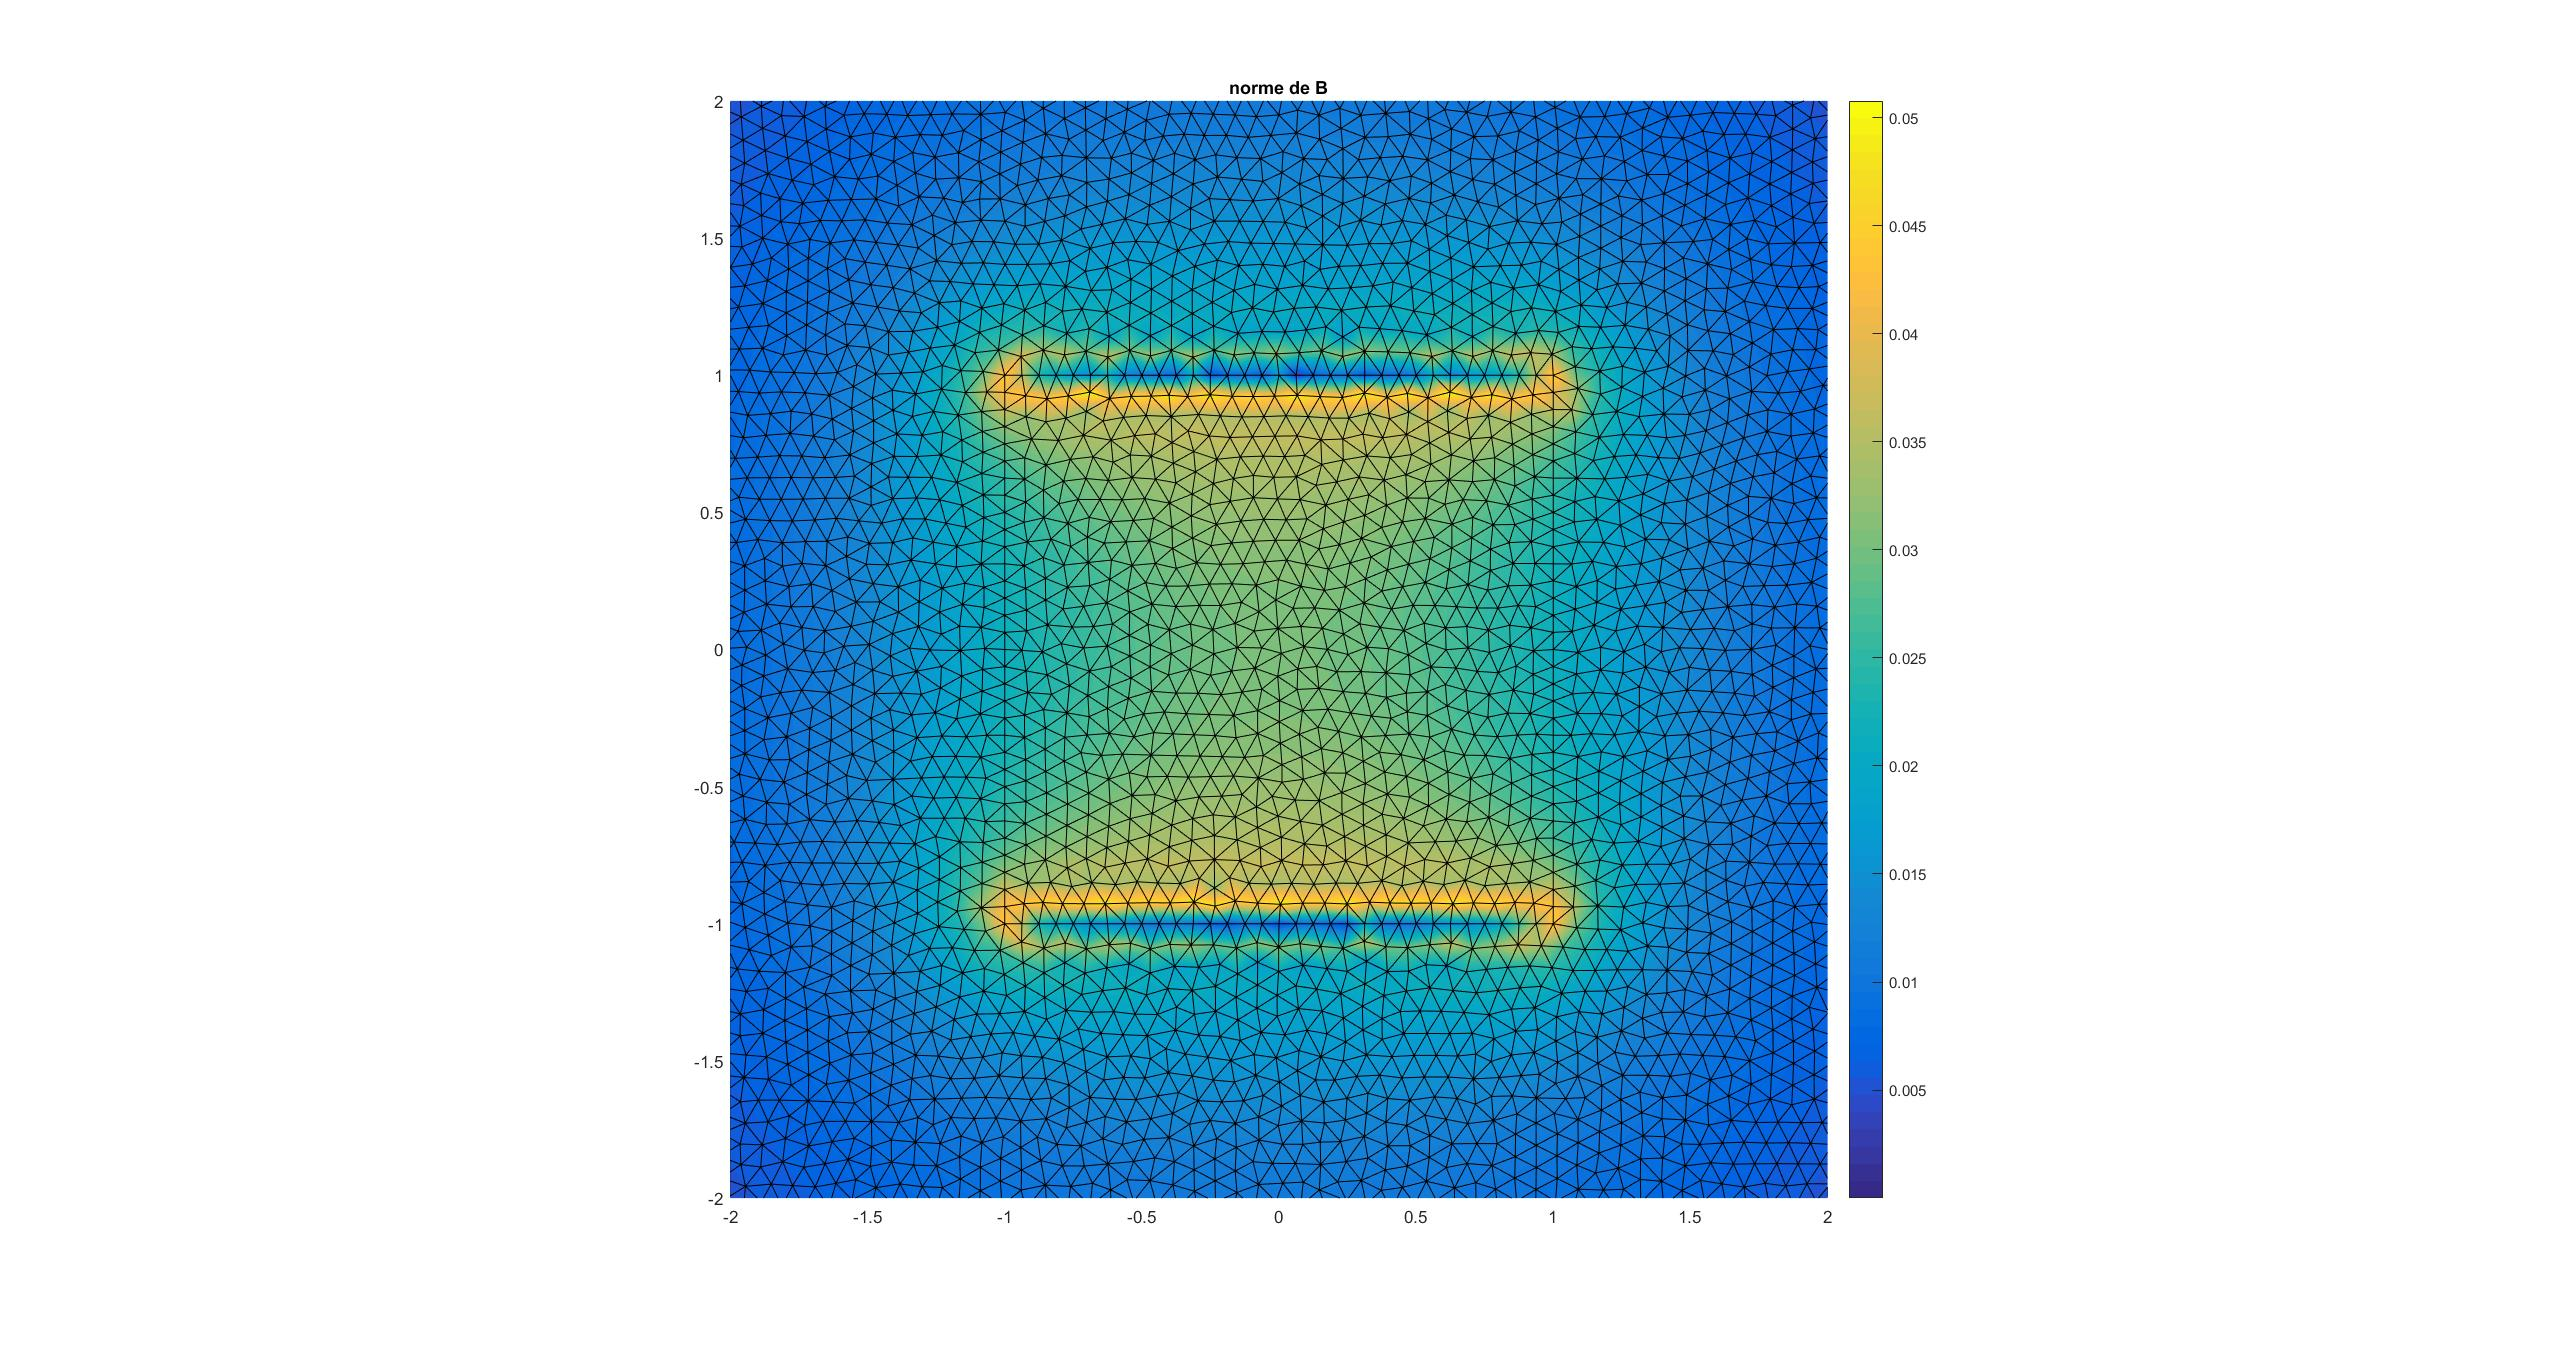
\includegraphics[height = 8 cm, keepaspectratio]{graphes/norme_du_champ.jpg}
\caption{norme du cham $\vec{B}$, fenêtre centrée sur [-2, 2]}
\label{figure 1}
\end{center}
\end{figure}
%=========================================================================================================================================================
%												chapitre 2 equations de Navier_Stockes
%=========================================================================================================================================================
\newpage
\chapter{Équations de  Navier Stokes} 
Nous allons à présent nous intéresser à la modélisation de l'écoulement, qui suit les équations de Navier-Stokes d'après les hypothèses que nous avons émis précédemment. 
Nous supposons que nous avons à notre disposition deux aimants, qui sont perpendiculaires sur les côtés de la cuve, l'un produit un champ $B_1$, l'autre produit un champ $B_2$
Le premier aimant va produire un tourbillon dans le fluide, le deuxième va produire deux tourbillons parallèles, qui sont orthogonaux au premier tourbillon . Tout cela dans le but d'obtenir un écoulement tourbillonnaire. 
\begin{figure}[!h]
\begin{center}
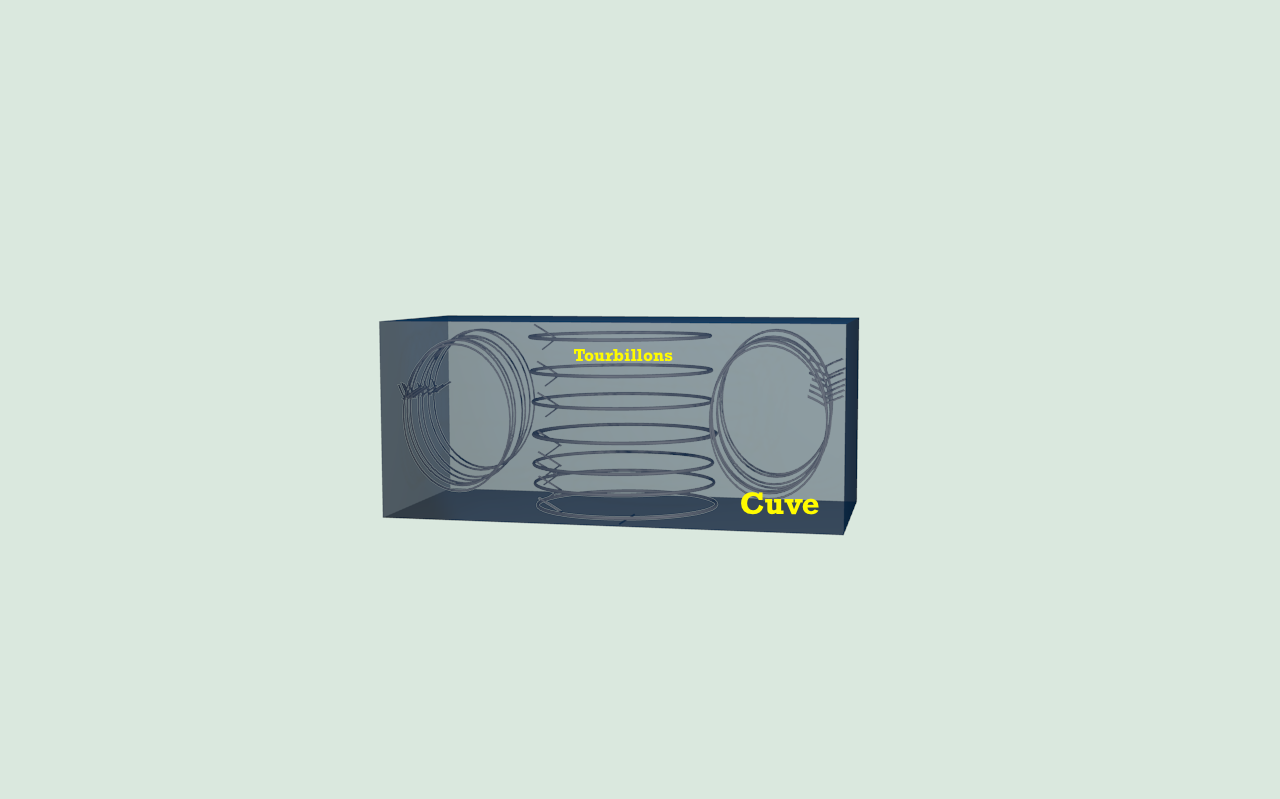
\includegraphics[height = 8 cm, keepaspectratio]{graphes/3_tourbillons.png}
\caption{les trois tourbillons que nous souhaitons obtenir avec notre dispositif expérimental}
\label{figure 1}
\end{center}
\end{figure}
%======================== Equations de Navier-stokes==========================================================
\newpage
\subsection{Équations de Stokes}

Le liquide est un conducteur placé dans un champ magnétique et parcouru par un courant supposé uniforme $\vec{j_0}$.
\normalsize 
Afin de pouvoir trouver l'équation de la trajectoire d’un point donné, on cherche tout d’abord à trouver la vitesse dans l'écoulement du fluide contenu dans un domaine $\Omega$.
\\A partir des équations de Navier-Stokes incompressibles, on détermine simultanément la vitesse  $V$ et la pression $P$. 
\\
\\
On émet les hypothèses suivantes :
\\
Dans un premier temps, nous pouvons négliger les forces d’inertie du fluide comme on a un faible nombre de Reynolds.
Le fluide visqueux est en mouvement le long d’une paroi solide fixe d’où une vitesse nulle sur le bord car 
$\vec{V_{\partial\Omega}}=\vec{V_{\text{paroi}}}=\vec{0}$
\\	
Finalement, on se place en régime stationnaire.
\begin{equation*}
  \left\{
    \begin{aligned}
      &\vec{0}=-\vec{\bigtriangledown}P +\mu\vec{\Delta}V +\vec{f}\;\text{dans }\Omega \\
      &\text{div}(\vec{V})=0\;\text{dans }\Omega \\     
      &\vec{V}=\vec{0}\;\text{sur }\partial\Omega
    \end{aligned}
  \right.
\end{equation*}

La force $\vec{f}$ correspond à la force de Laplace induite par le champ magnétique. La densité volumique de cette force est donnée par :
\[
\begin{aligned}
	\vec{f}=\vec{j_0}\land\vec{B}&=j_0\times M_0\times \vec{j}\wedge \vec{B^*} \\
	 \vec{B^*} =\frac{\vec{B}}{M_0}, 
	\ &\text{et} \ j_0=\frac{\Delta E}{L}\sigma
	\\
\text{avec} \quad
&\sigma : \text{la conductivité du fluide }
\\%
&\text{L: la longueur de base de la cuve} \\
&\Delta E : \text{la différence de potentiel}
\end{aligned} \\
\]
Ainsi on peut calculer la force magnétique pour un champ magnétique $\vec{B_1}$
\[
	\vec{B_1} = 
	\begin{pmatrix}
   		B_{1,x}\\
  		 B _{1,y}\\
  		 0
	\end{pmatrix} 
\]
\[
	\vec{f}=j_0\vec{e}_{x}
	\wedge\begin{pmatrix}
   		B_{1,x}\\
   		B _{1,y}\\
   		0
\end{pmatrix}=
j_0\times \begin{pmatrix}
  			0\\
   			0\\
    		B_{1,y}
			\end{pmatrix} 
\]

%==================================================== Adimensionnement de l'équation de Stokes ============================================================

\subsection{Adimensionnement de l'équation de Stokes}

\normalsize Afin de résoudre un seul système indépendamment des constantes, on adimensionne l'équation de Stokes. Le régime stationnaire sera pris en compte après adimensionnement.
\\%
Posons :
\begin{equation*}
\vec{V'}(x,t)=\frac{\vec{V}(x,t)}{V_0}\;;\vec{x'}=\frac{\vec{x}}{L_0}\; ; \vec{f'}(\vec{x'})=\frac{\vec{f}(\vec{x})}{j_0M_0}\;;P'=\frac{P}{P_0}\; ;t'=\frac{t}{\frac{L_0^2}{\mu}}\;
\end{equation*}
En injectant dans l'équation de Stokes d'évolution :
\begin{equation*}
  \left\{
    \begin{aligned}
    \rho\frac{\partial \vec{V}}{\partial t}=-\vec{\bigtriangledown} P + \mu \vec{\Delta}\vec{V}+\vec{f}
        \end{aligned}
  \right.
\end{equation*}
il en résulte :
\begin{equation*}
  \left\{
    \begin{aligned}
    \frac{\partial \vec{V'}}{\partial t}=-\frac{L_0 P_0}{\rho \mu V_0}\vec{\bigtriangledown} P '+  \vec{\Delta}\vec{V'}+\frac{L_0^2j_0M_0}{\mu V_0}\vec{f'}
        \end{aligned}
  \right.
\end{equation*}
On adimensionne par rapport à $V_0$ et $P_0$ de sorte que $\frac{L_0 P_0}{\rho \mu V_0}=1$ et $ \frac{L_0^2j _0M_0}{\mu V_0}=1$, le régime stationnaire étant établi:
\[
      \vec{0}=-\vec{\bigtriangledown}P' +\vec{\Delta}V' +\vec{f'}\;\text{dans }\Omega 
\]

%================= Formulation variationnelle =========================================================
\subsection{Formulation variationnelle}

Afin d'obtenir la formulation variationnelle de l'équation de Stokes, on passe dans l'espace des distribution de sorte que pour toute fonctions test $\varphi$ on a 
\[
	\int_\Omega\vec{\bigtriangledown}P'\times \vec \varphi=\int_\Omega-\mu\vec{\Delta}V'\times \vec \varphi +\int_\Omega\vec{f'}\times \vec \varphi 
\]
En appliquant la formule de Green, on obtient :

\[
\forall \varphi \in D(\Omega) \quad  \int_\Omega\vec{\bigtriangledown}P'. \vec \varphi + \int_{\Omega}\bigtriangledown V'. \bigtriangledown \varphi = \int_\Omega\vec{f'}. \vec \varphi
\]
Comme précédemment nous nous plaçons dans l'espace $V_{h}$ d'approximation polynomiale.
Nous pouvons ainsi décomposer les champs de pression $P'$, la vitesse $V'$ et la force $\vec{f'}$ dans la base des $(\varphi_{i})$:

\begin{equation*}
  \left\{
    \begin{aligned}
 &V '= \sum_{i=1}^{N_{h}}{\ V_{i}\varphi_{i}} \text{ \ \ où } V_{i} = V(P_{i}),\  i= 1,2,...,N_{h}\\
 &P '= \sum_{i=1}^{N_{h}}{\ P_{i}\varphi_{i}} \text{ \ \ où } P_{i} = P(P_{i}),\  i= 1,2,...,N_{h}\\
 &f' = \sum_{i=1}^{N_{h}}{\ f_{i}\varphi_{i}} \text{ \ \ où } f_{i} = f(P_{i}),\  i= 1,2,...,N_{h}\\
\end{aligned}
  \right.
\end{equation*}$ $ \\ 
On prend $\varphi\ =\ \varphi_{i}$ un vecteur de la base
\begin{equation*}
  \left\{
    \begin{aligned}
	&\int_{\Omega}\bigtriangledown V_{h}.\bigtriangledown \varphi\ 
	=\ 
	\sum_{i, j \in [1, N_{h}]^{2}} \int_{\Omega}V_{i}\bigtriangledown\varphi_{i}. \bigtriangledown\varphi_{j} 
	= 
	\sum_{i,j \in [1, N_{h}]^{2}} A_{ij} V_{i}\\
	&\int_{\Omega}\bigtriangledown P_{h}.\varphi\ 
	=\ 
	\sum_{i, j \in [1, N_{h}]^{2}} \int_{\Omega}P_{i}\bigtriangledown\varphi_{i}. \varphi_{j} 
	= 
	\sum_{i,j \in [1, N_{h}]^{2}}C_{ij} u_{i}\\
	&\int_{\Omega} f. \varphi\ 
	=\ 
	\sum_{i, j \in [1, N_{h}]^{2}} \int_{\Omega}f_{i}\varphi_{i}. \varphi_{j} 
	= 
	\sum_{i,j \in [1, N_{h}]^{2}} M_{ij} f_{i}\end{aligned}
  \right.
\end{equation*}
On peut donc écrire la formulation variationnelle sous la forme d'un problème linéaire:
\begin{equation*}
  \left\{
    \begin{aligned}
	&-A\times V + C \times P = M	\times f \ \text{sur} \ \Omega\\
	& C\times V = 0 \ \text{sur} \  \partial\Omega\\
	\end{aligned}
  \right.
\end{equation*}

%====================== principe de superposition 
\subsection{Principe de superposition}

La linéarité de l'équation nous permet d'appliquer le principe de superposition est donc de décomposer la résolution du problème en deux résolutions : une pour chaque terme source et ensuite de les sommer.
Pratiquement nous allons résoudre le problème en deux temps : d'un coté pour l'aimant centré qui donne deux tourbillons et d'autres part pour l'aimant décentré qui donne un tourbillon pour ensuite sommer les champs de vitesse après transposition du champ pour l'aimant décentré pour se retrouver dans la configuration où les tourbillons sont perpendiculaires.
\begin{figure}[!h]
	\begin{center}
	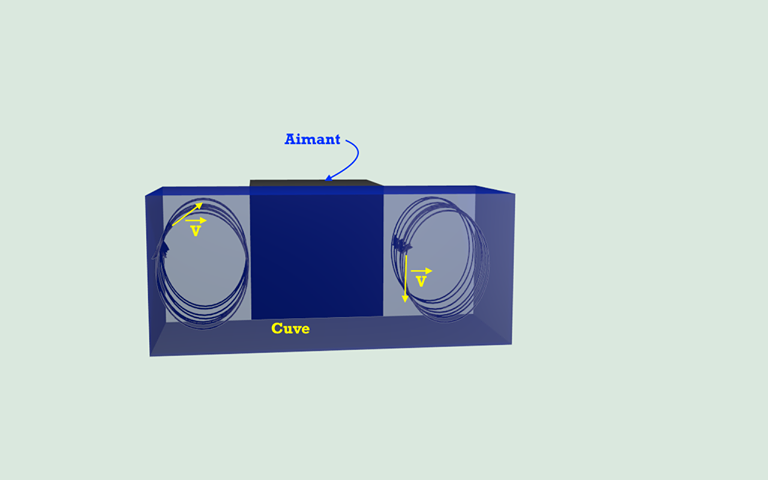
\includegraphics[height = 8 cm, keepaspectratio]{graphes/config_centre.png}
	\caption{résolution pour un aimant centré}
	\label{figure 1k}
	\end{center}
\end{figure}
\begin{figure}[!h]
	\begin{center}
	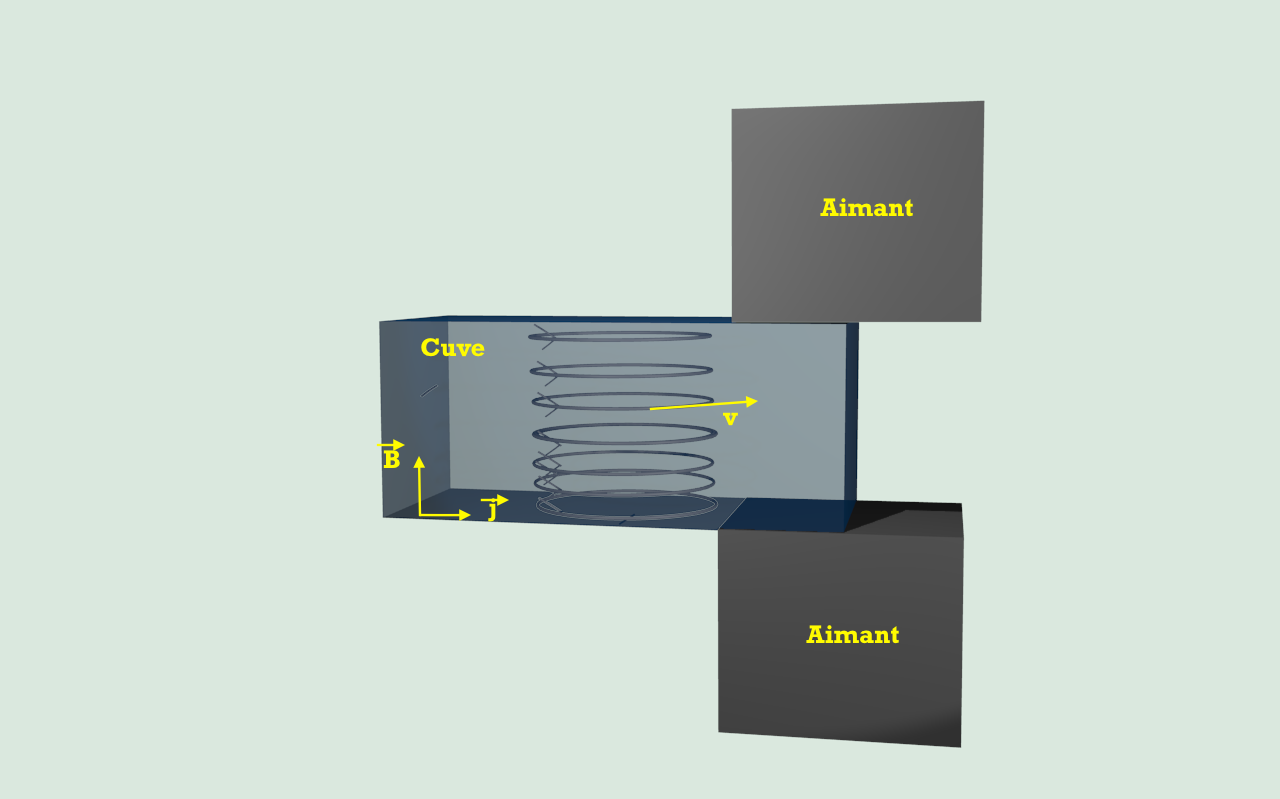
\includegraphics[height = 8 cm, keepaspectratio]{graphes/champvec2.png}
	\caption{résolution pour seux aimants decentrés après transposition du champ de vitesse pour que les tourbillons soient perpendiculaires}
	\label{figure 1h}
	\end{center}
\end{figure}
%===================== implementation algorithmique =======================================
\newpage
\subsection{Implémentation algorithmique}

Nous allons à présent mettre en place les calculs précédents de manière numérique sur Matlab en maillant le domaine de résolution qui est ici la cuve qui accueille le fluide .  
\\ 
On pose $ L_x,  L_y,  L_z$ les dimensions de la cuve selon x, y, et z.
\newline
Le domaine $\Omega = [0, L_x]\times[0, L_y]\times[0, L_z]$ est ainsi discrétisé par un maillage uniforme défini par les points : 
\\

\[
\left\{
\begin{array}{ccc}
  x_{ij} = (\frac{i\times L_x}{N+1} ,\frac{j\times L_x}{N+1}),    i,j=0,1,......,N+1\\
  y_{ij} = (\frac{i\times L_y}{N+1} ,\frac{j\times L_y}{N+1}),    i,j=0,1,......,N+1  \\
 z_{ij} = (\frac{i\times L_z}{N+1} ,\frac{j\times L_z}{N+1}),    i,j=0,1,......,N+1  
\end{array}
\right.
\]
\begin{figure}[!h]
	\begin{center}
	\centering
		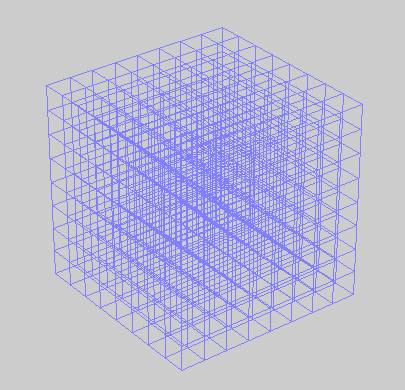
\includegraphics[height = 8cm, keepaspectratio]{graphes/maillage_droit.png} 
		%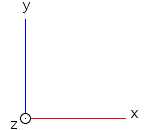
\includegraphics[height = 2cm, keepaspectratio]{graphes/axes.png}
		\caption{maillage du domaine de résolution de coté 1 en prenant 11 points dans les directions x, y, et z à l'aide de la fonction matlab $ndgrid$}
	\end{center}
\end{figure}

%============================= calcul champ de vitesse =====================================
\newpage
\subsection{Calcul des matrices du système linéaire en trois dimensions}

Cette partie va reposer sur le même principe que les calculs en deux dimensions et s'appuie sur le cours "Analyse numérique des équations de
Navier-Stokes" de J.-F Scheid.

En effet comme précédemment, nous allons nous appuyer sur des matrices élémentaires comprenant les contributions des différents noeuds sur chaque élement en nous ramenant à un élément de référence.  \\
Nous cherchons à calculer les matrices de rigidité A et de masse M.
Les éléments de la matrice élementaire pour la matrice de rigidité sur un élément $K$ sont les 
\[
W_{i,j}^{k,l}=\int_K \frac{\partial l^{(i)}}{\partial x_k} \times \frac{\partial l^{(j)}}{\partial x_l}dx
\]
où les  $\l^{(i)}$ sont les fonctions de base des élements du maillage comme précédemment dans la partie 2D. \\
Et pour la matrice de masse la matrice élémentaire sur un élément K est
\[
M_{i,j}=\int_K l^{(i)}\times l^{(j)}dx
_K 
\]
 Pour déterminer ces intégrales, on se ramène à l'élément de référence $\hat{K}$ avec la transformation affine
$F_K(\hat{x})=B_K \hat{x} + b_K$.
\\
\\
De la même manière que les travaux précédents pour les transformations entre les éléments de référence, on arrive à :
\[
\hat{\bigtriangledown}\hat{v}(\hat{x})= [DF_K(\hat{x})]^T\times \bigtriangledown v(x)
\]
avec $[DF_K(\hat{x})]$ la matrice jacobienne de $F_K$ dont on note les éléments $J_{i,j}$, et ainsi on a $\bigtriangledown v(x) = [B_K^{-1}]^T\hat{\bigtriangledown} \hat{v}(\hat{x})$.

On obtient l'expression des éléments de la matrice élementaire en fonction des valeurs sur l'éléments de référence $\hat{K}$.
\[
W^{k,l} = \frac{1}{|\text{det} \ B_K|}\sum_{m,n=1}^{N} J_{km}\ J_{ln}\ \hat{W}^{m,n}
\]
En regardant la construction des éléments avec les tables de connectivité on voit que les matrices élémentaire de réference sont de taille $9\times 9$ que l'on sait calculer explicitement.
Dans notre algorithme on calcule la matrice de rigidité à l'aide du script $matrix3D$ qui réunit dans des matrice $27\times 27$ les termes croisés des matrices élémentaires ce qui permet de calculer directement en une affectation la matrice de rigidité en utilisant ses propriétés de symétries par blocs.

Pour la matrice élémentaire de masse nous pouvons développer des calculs similaire à ceux menés dans le cas 2D pour trouver une matrice élémentaire $M_{i, j} = |\text{det} J| \times PhiPhi$ où $|\text{det} J|$ est le déterminant du Jacobien et $PhiPhi$ une matrice déterminé qui reste la même à chaque itération.

On utilise ainsi dans les scripts de calculs une méthodologie similaire consistant à stoker les indices des valeurs comprises dans les matrices élémentaires et à construire la matrice complète à la fin des itérations sur les éléments en assignant les valeurs dans la matrices aux indices justement indiqués par les nœuds que l'on a gardé en mémoire en une seule affectation.

\begin{verbatim}
point=t(k,:);
indice=point';
detB=((v(t(k,2),1)-v(t(k,1),1)).*...
(v(t(k,4),2)-v(t(k,1),2)).*(v(t(k,5),3)-v(t(k,1),3)));
    
DxDxval=detB.*(1./(v(t(k,2),1)-v(t(k,1),1)).^2).*DxDx;
  
DyDzval=detB.*(1./((v(t(k,4),2)-v(t(k,1),2)).*...
    (v(t(k,5),3)-v(t(k,1),3)))).*DyDz;
DxWval=detB.*(1./(v(t(k,2),1)-v(t(k,1),1))).*DxW;
DyWval=detB.*(1./(v(t(k,4),2)-v(t(k,1),2))).*DyW;
DzWval=detB.*(1./(v(t(k,5),3)-v(t(k,1),3))).*DzW;
    
AddMatElem(A,indice,indice,2*nu*DxDxval+nu*DyDyval+nu*DzDzval);
AddMatElem(A,indice+nv2,indice+nv2,nu*DxDxval+2*nu*DyDyval+nu*DzDzval);
AddMatElem(A,indice+2*nv2,indice+2*nv2,nu*DxDxval+nu*DyDyval+2*nu*DzDzval);
\end{verbatim}
%================= implementation algo =============================================================
\subsection{Raccordement à la modélisation du champ magnétique}

Pour résoudre le système linéaire qui découle des équations de Navier-Stokes, nous devons reprendre notre travail précédent pour former le second terme $f$, matrice colonne regroupant les valeurs scalaires de la force magnétique aux différents point du maillage.

Nous devons donc faire le liens entre le maillage de résolution en trois dimension pour la résolutions des équations régissant l'écoulement et le maillage en deux dimensions sur lequel on calcule le champ magnétique. 

Comme nous l'avons énoncé, nous supposons que le champ magnétique est invariant selon le troisième dimensions, il est donc inutile de le recalculer pour chaque 'couche' du maillage 3D, d'autant plus que le maillage 3D est uniforme. 
La méthodologie que nous allons donc appliquer consiste à calculer une unique fois le champ magnétique sur une seule couche de maillage (la couche z = 0 en partique dans l'algorithme) et reprendre les valeurs du champ sur les autres couches.

Ce que nous faisons en pratique est de générer un grand maillage de résolutions 2D pour calculer le champ magnétique, ce qui permet d'atténuer les effets de bord subit par le champ magnétique. 
\newline
Nous utilisons ensuite la fonction Matlab $delaunay$ qui permet à partir du maillage rectangulaire, de définir un maillage triangulaire (comme nous avons travaillé sur un maillage de type triangulaire quelconque auparavant pour le calcul du champ magnétique).
Nous identifions ensuite sur ce maillage de résolution 2D un domaine correspondant à la cuve est un domaine correspondant à l'aimant, en fonction de la configuration choisie. Le maillage sur le domaine assigné à la cuve doit bien sur correspondre à une couche du maillage de résolution 3D utilisé pour la résolution des équations de Navier-Stokes.

\begin{figure}[!h]
	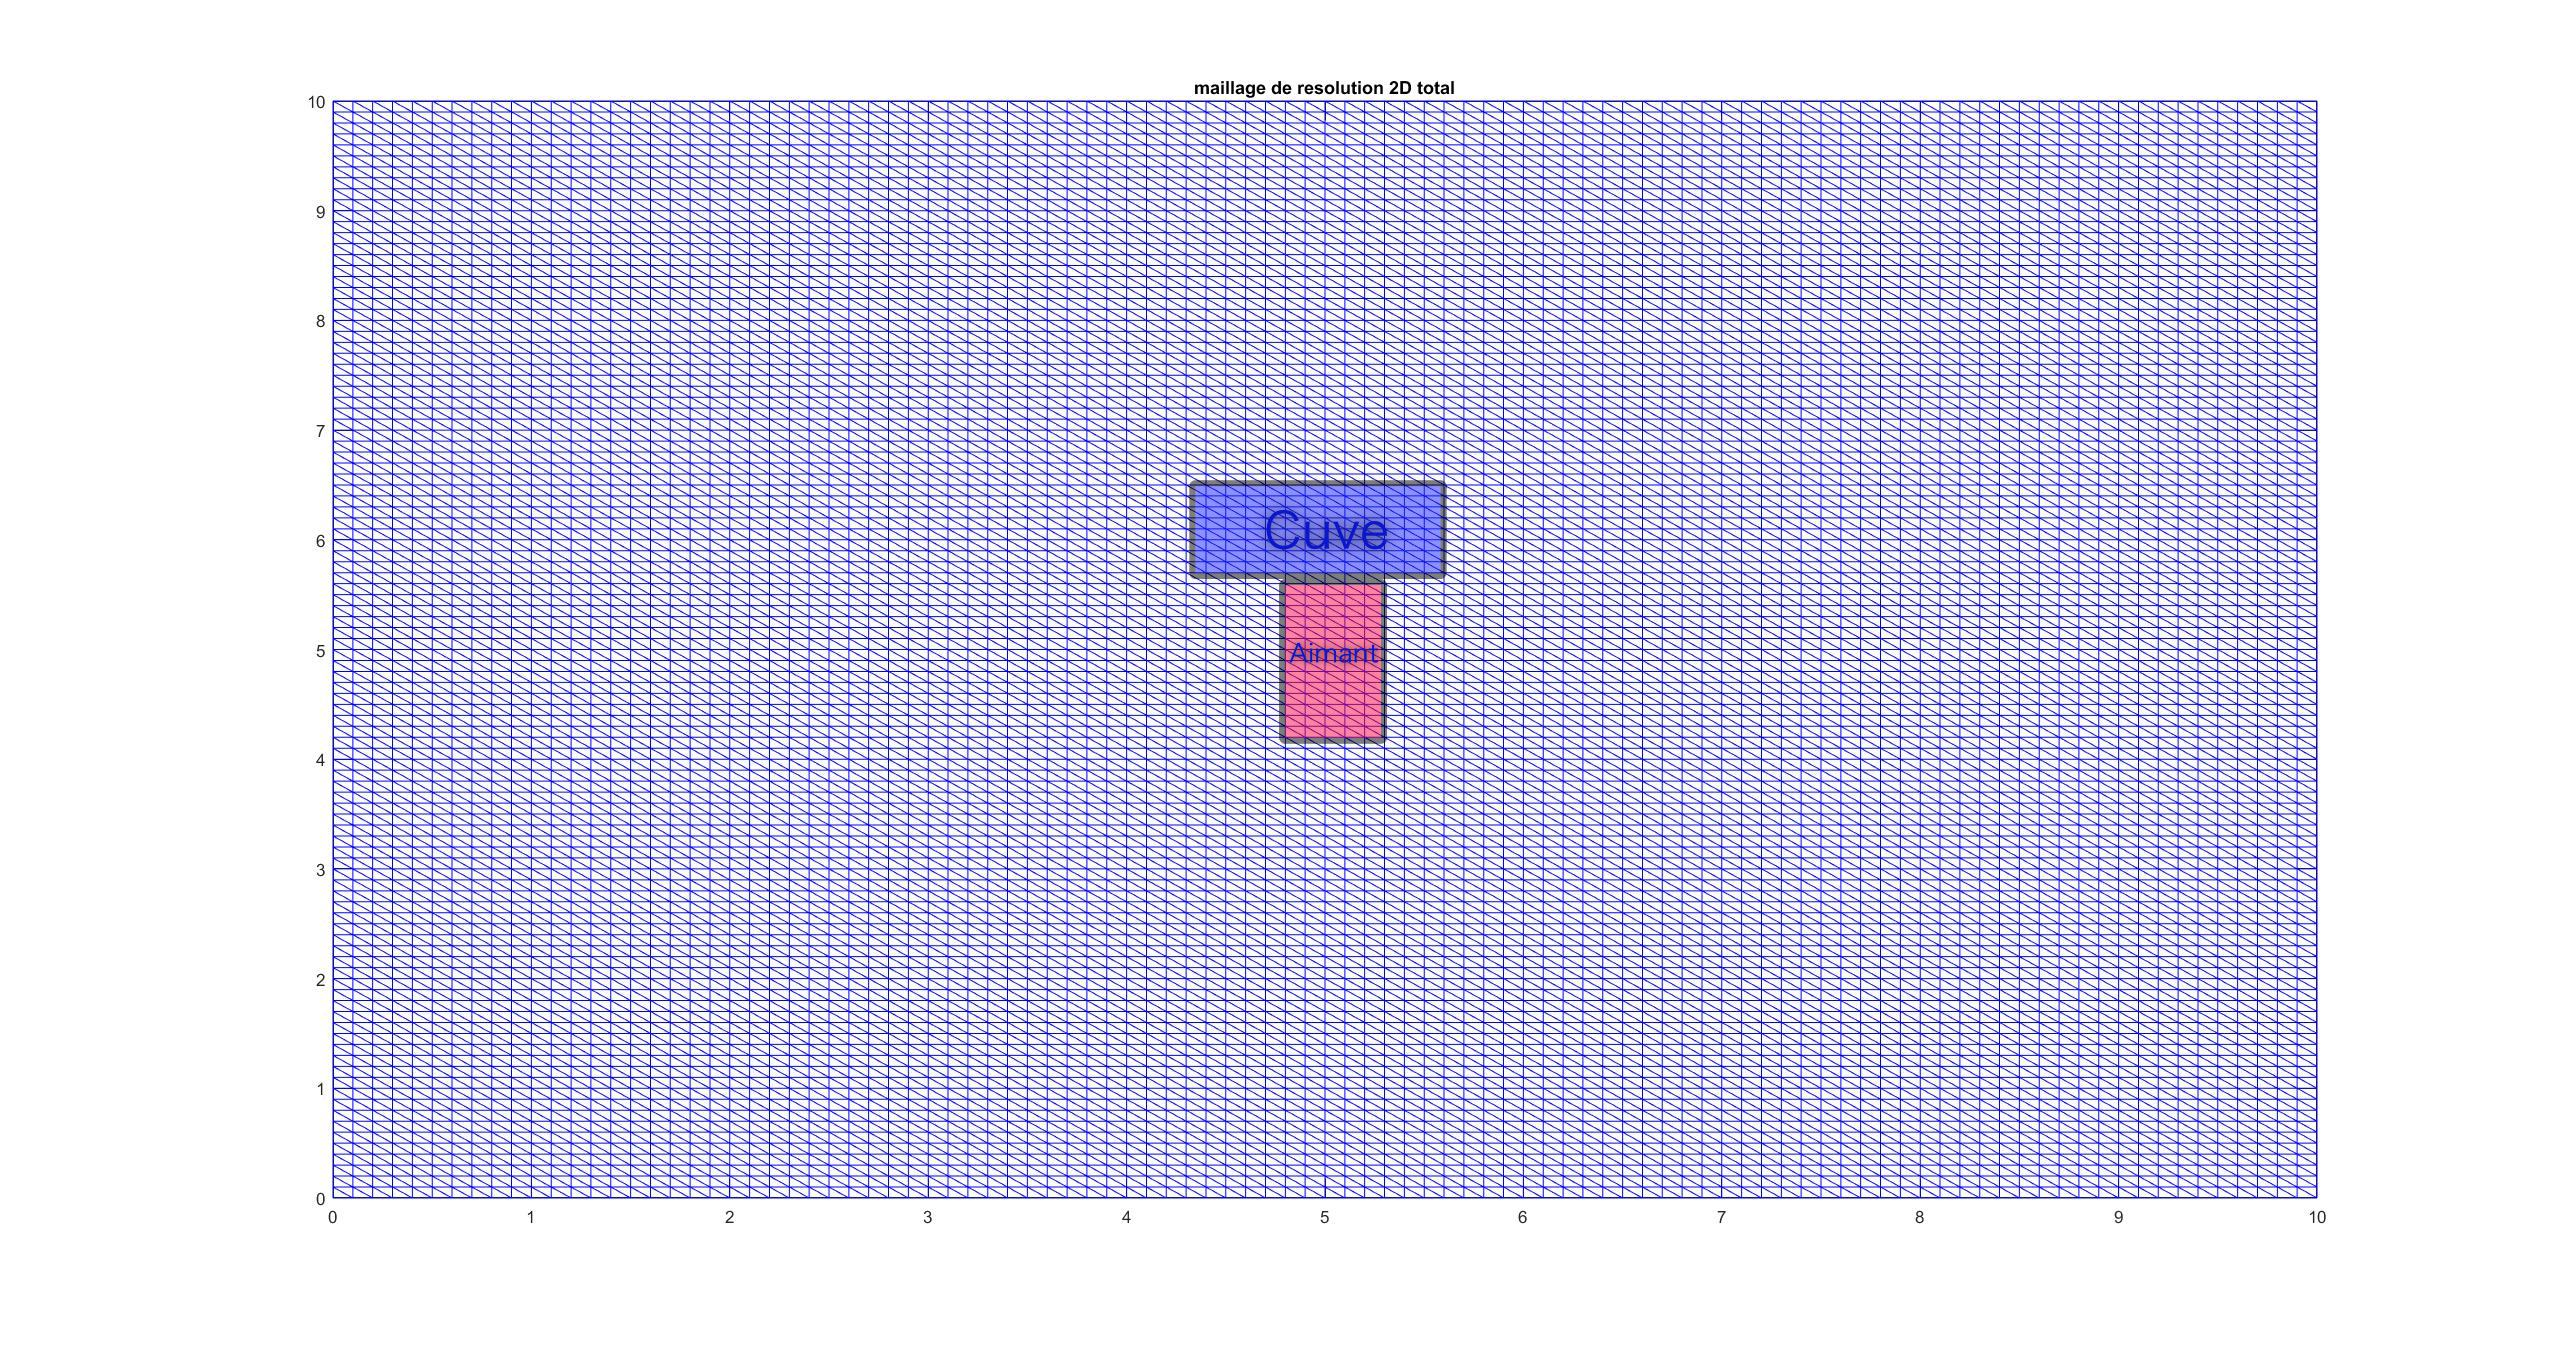
\includegraphics[height = 8cm, keepaspectratio]{graphes/maillage_resolution_total_centre.jpg}
	\caption{\label{figure 3z } configuration dans le cas de la résolution pour la configuration avec l'aimant centré}
\end{figure}
\begin{figure}[!h]
	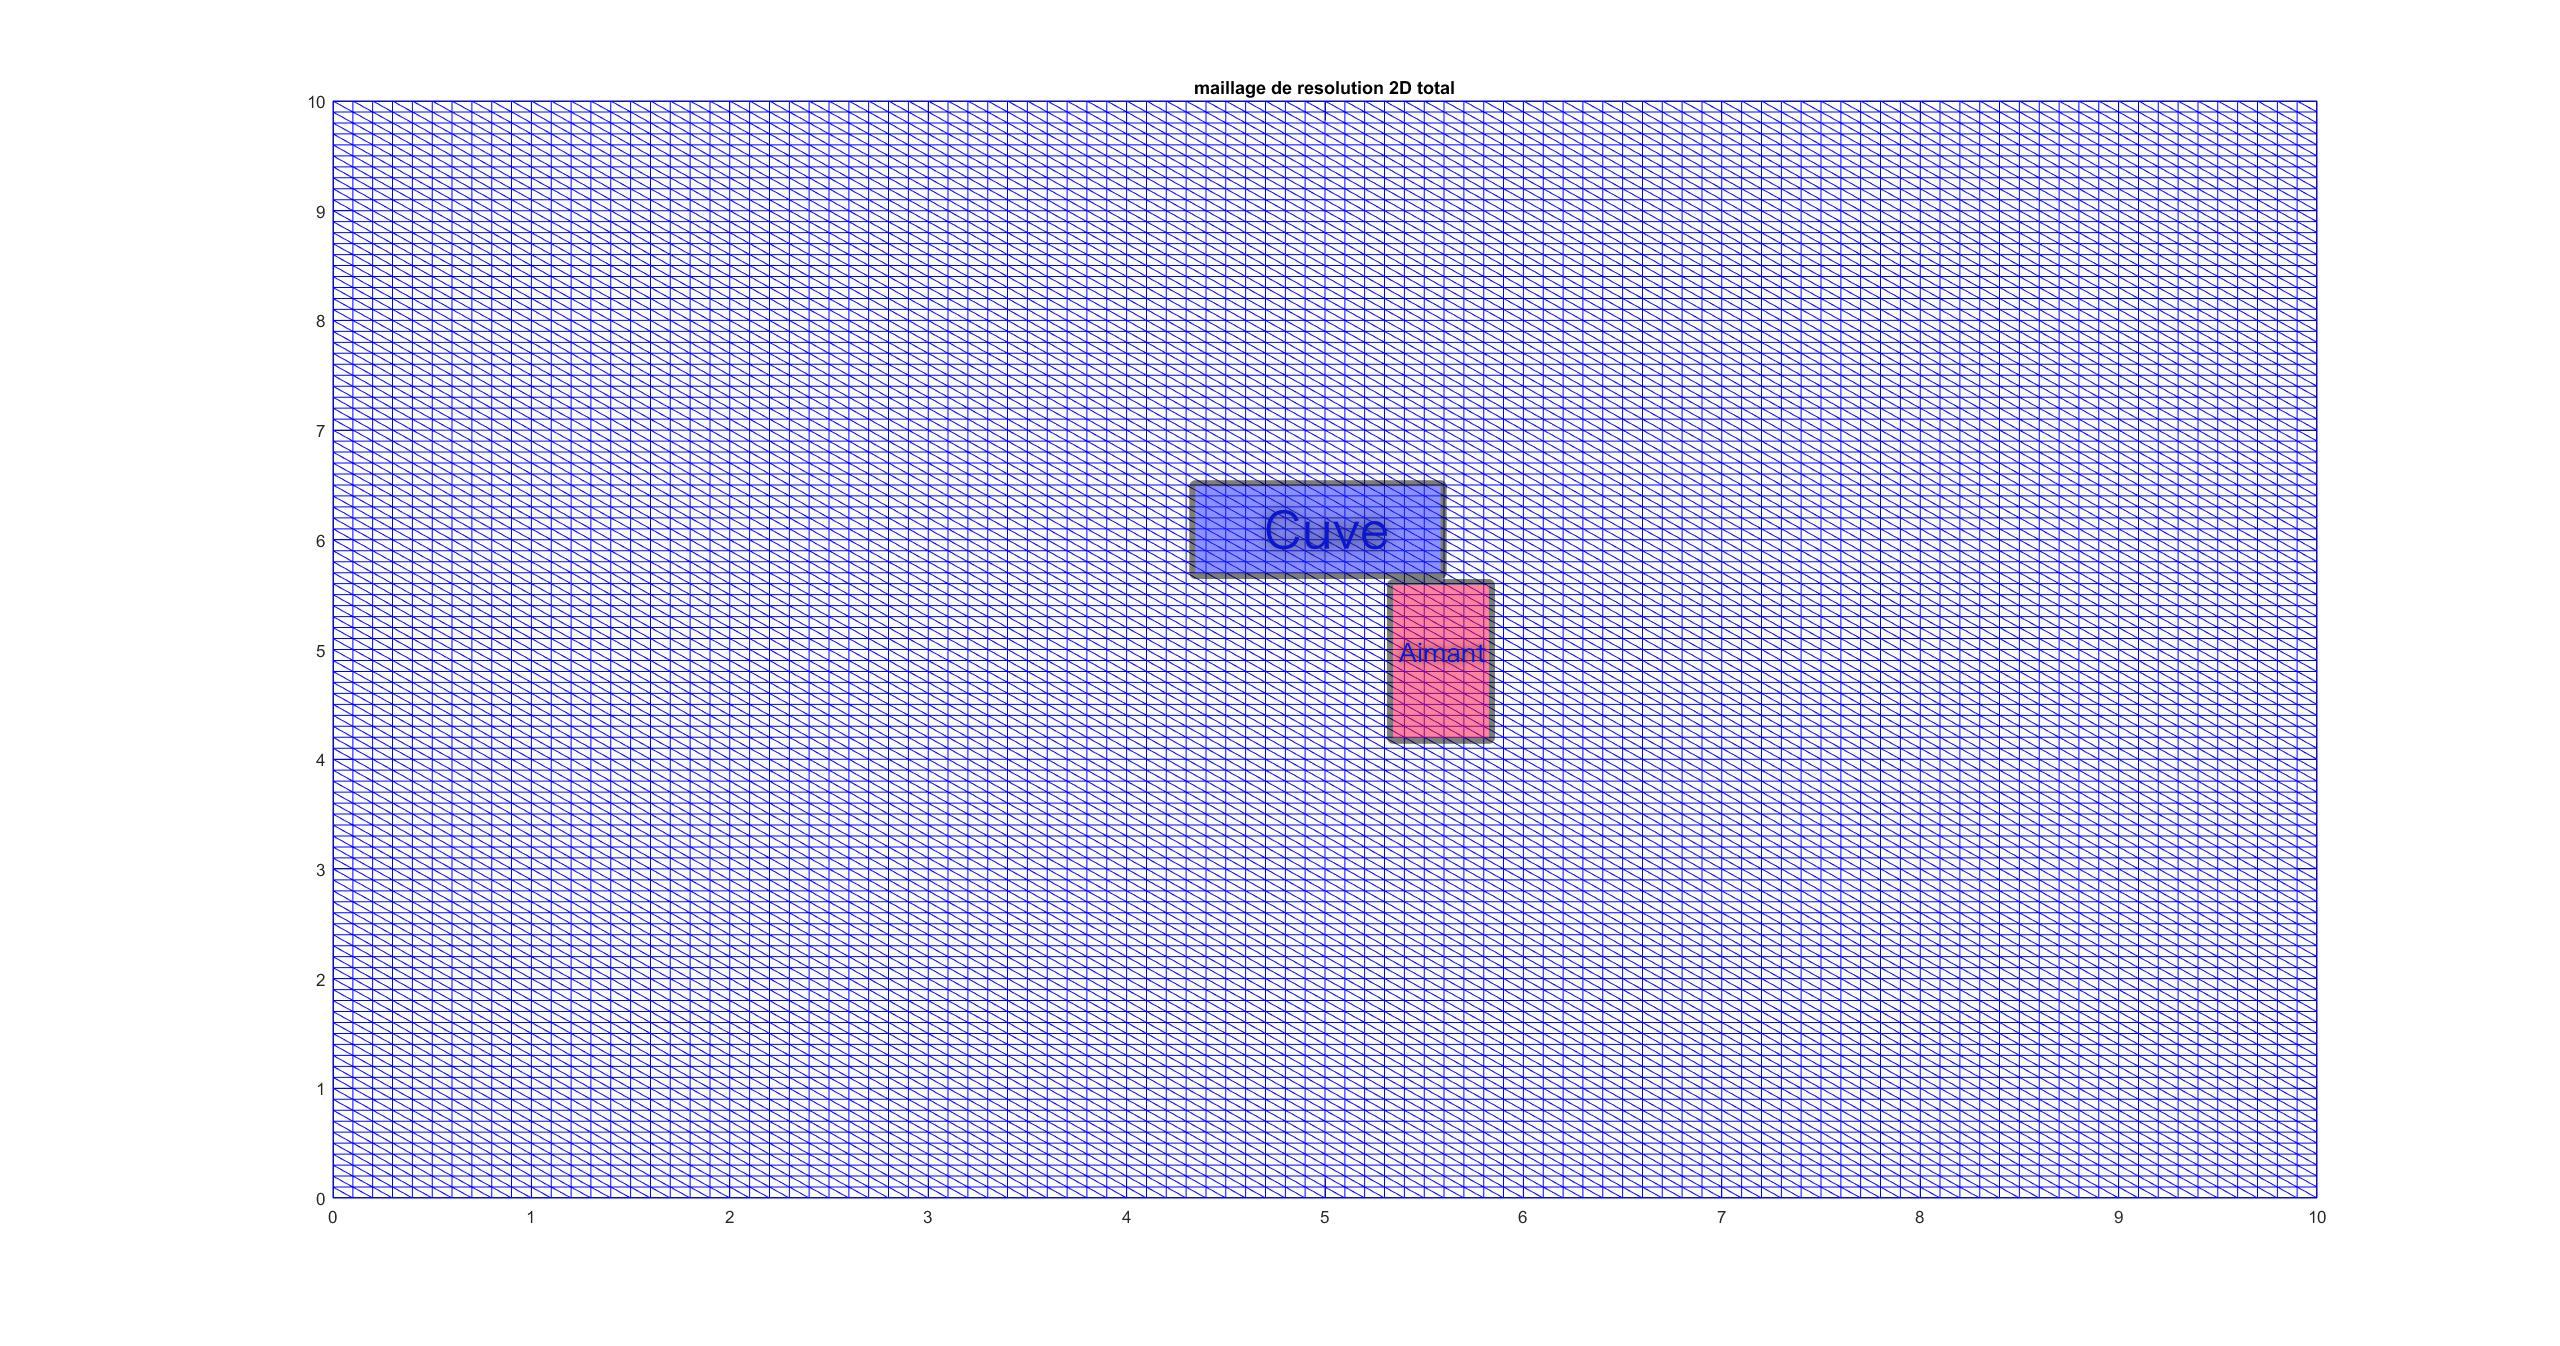
\includegraphics[height = 8cm, keepaspectratio]{graphes/maillage_resolution_total_decentre.jpg}
	\caption{\label{figure 3r } configuration dans le cas de la résolution pour la configuration avec l'aimant décentré}
\end{figure}

\newpage
Algorithmiquement, pour assigner les différents domaines du maillage de résolution 2D générés, nous utilisons le vecteur label $fnum$ qui prend sur chaque triangle la valeur 1, 2, ou 3 en fonction du domaine qui lui a été assigné.
\newline
Maintenant  notre objectif est de pouvoir adapter les données extraites à l'algorithme de Stokes 3D. Le premier obstacle est de réindexer le numéro des triangles pour qu'il y ait une bonne consistance des données lorsque l'algorithme va les utiliser: il faut renuméroter les triangles dans l'ordre. 
\newline  	

Un autre point important est le degré d'interpolation des espace polynomiaux sur lesquels nous travaillons. En effet nous avons résolu les équations du champ magnétique avec des éléments finis de degrés d'interpolation polynomiales 1 (éléments P1), alors que la résolution des équations de Navier-stokes nécessite des éléments finis P2. Il faut donc doubler le nombre de points d'interpolations du champ magnétique avant d'injecter le second membre $f$ dans l'algorithme de résolution des équations de Navier Stokes. Les données prennent alors une nouvelle structure suite à ce dédoublement des point, les matrices ne suivent plus le sens de parcourt des données fixé avec la fonctions de génération de maillage $ngrid$(qui est une généralisation sur la troisième dimension  de $meshgrid$). Ce doublement de point du maillage avec la génération des tables nouvelles tables de descriptions du maillage t et v sont faite par la fonction $mesh_3D$ fournis par M. Scheid que nous utilisons comme une boite noire.

On le voit tout de suite un affiche $triplot$ après avoir appliqué $delaunay$ sur les données de la couche 2D du maillage 3D dont on a doublé les points.
\begin{verbatim}
z = 0;   % niveau z = 0
indz = find(v(:,3) == z);		% récupération des indices des nœuds pour le niveau 0
xz = v(indz,1); yz = v(indz,2); vz = [xz, yz];
tz = delaunay(xz,yz);               % triangulation de Delaunay 
triplot(tz,xz,yz);   				% affichage
\end{verbatim}

\begin{figure}[!h]
	\center
	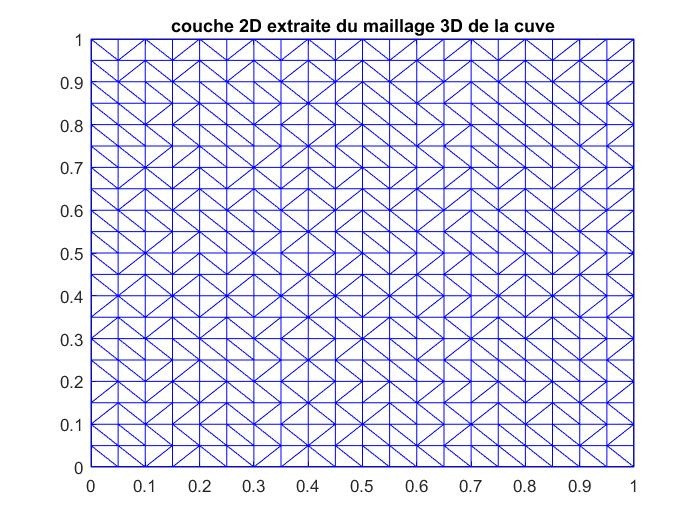
\includegraphics[height = 8cm, keepaspectratio]{graphes/affichage_extraction_2D.jpg}
	\caption{\label{figure 3 } affichage avec $triplot$ du maillage extrait}
\end{figure}
Si on compare à une structure de données classique généré avec $meshgrid$ ou $linspace$:
\begin{verbatim}
t_total_2D = delaunay(v_total_2D(:,1),v_total_2D(:,2)); 
triplot(t_total_2D ,X_total_2D,Y_total_2D);
xlim([4.5 5.5]);
ylim([4.5 5.5]);
\end{verbatim} 
\begin{figure}[!h]
	\center
	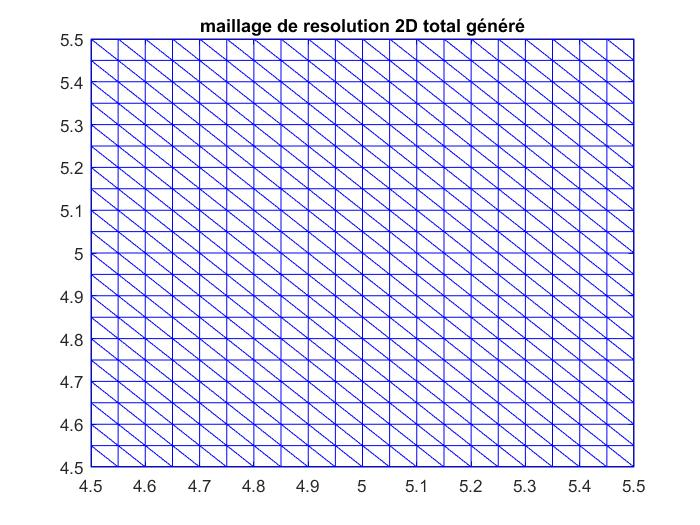
\includegraphics[height = 8cm, keepaspectratio]{graphes/affichage_extraction_2D_normal.jpg}
	\caption{\label{figure 37 } affichage avec $triplot$ du maillage extrait}
\end{figure}
\newpage
Pour comprendre la structure des données il faut alors se rapporter  aux tables de connectivité pour le type de maillage 3D généré.
\begin{figure}[h]
\center
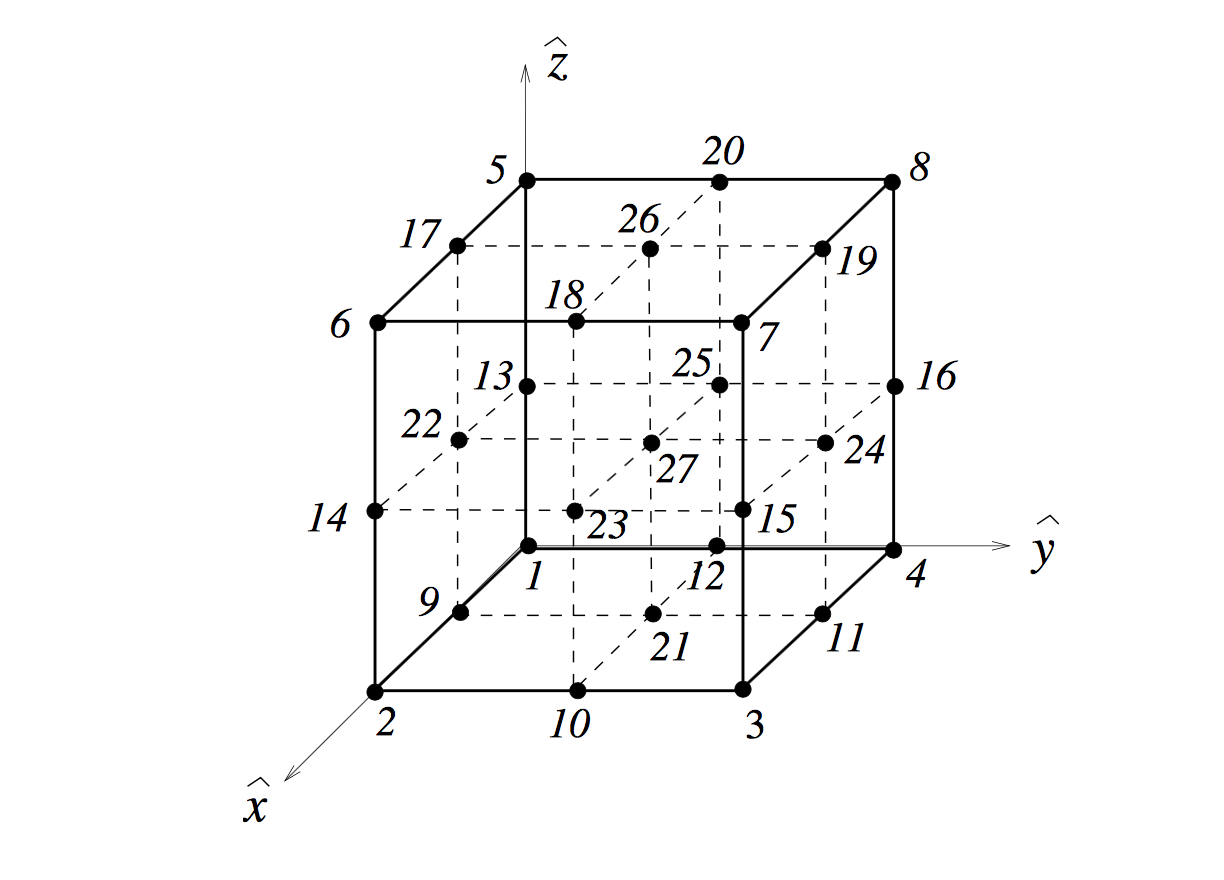
\includegraphics[height = 8cm, keepaspectratio]{graphes/table_de_connectivite.png} 
\caption{\label{figure 38 } table de connectivité, issu du cours $Analyse$ $numérique$ $des$ $équations$ $de$ $Navier$-$Stokes$, J.-F. Scheid}
\end{figure}
On comprend alors que cette structure des données ératique est du à l'arrangement de la tables de coordonnées v. Cela ne pose pas de problème dans la mesure où nous prenons garde à garder la même structure de données tout de long de notre algorithme de résolution et donc d'arranger selon la même structure le second membre $f$.
Et de même pour pouvoir visualiser graphiquement nos résultat nous devons passer de cette structure particulière des données à une structure compatible à l'affichage avec la fonction matlab $quiver3$.
 
%================= résultats ====================================================================
\newpage
\subsection{Résultats}
Nous allons étudier graphiquement les différents résultats que nous avons obtenus et évaluer leur justesse en les interprétants physiquement par rapport à ce que nous attendrions avec les paramètres donnés.
\newline
\\
Tout d'abord dans la configuration pour un aimant centré nous observons sur la coupe clairement deux tourbillons symétrique de part et d'autres de l'aimant, ce qui est logique comme la configuration est symétrique selon le même plan de symétrie, ce qui valide le bon placement des données dans la résolution du problème.
\\
Dans un premier temps, on discerne bien pour la première figure les deux tourbillons selon y, avec une forte vorticité au centre, car il s'agit du courant induit par les 2 tourbillons adjacents.
On utilise l'outil $StreamTracer$ de Paraview pour traver la trajectoire de particules à partir du champ de vitesse que nous avons obtenus en sortie.

\begin{figure}[!h]
\begin{center}
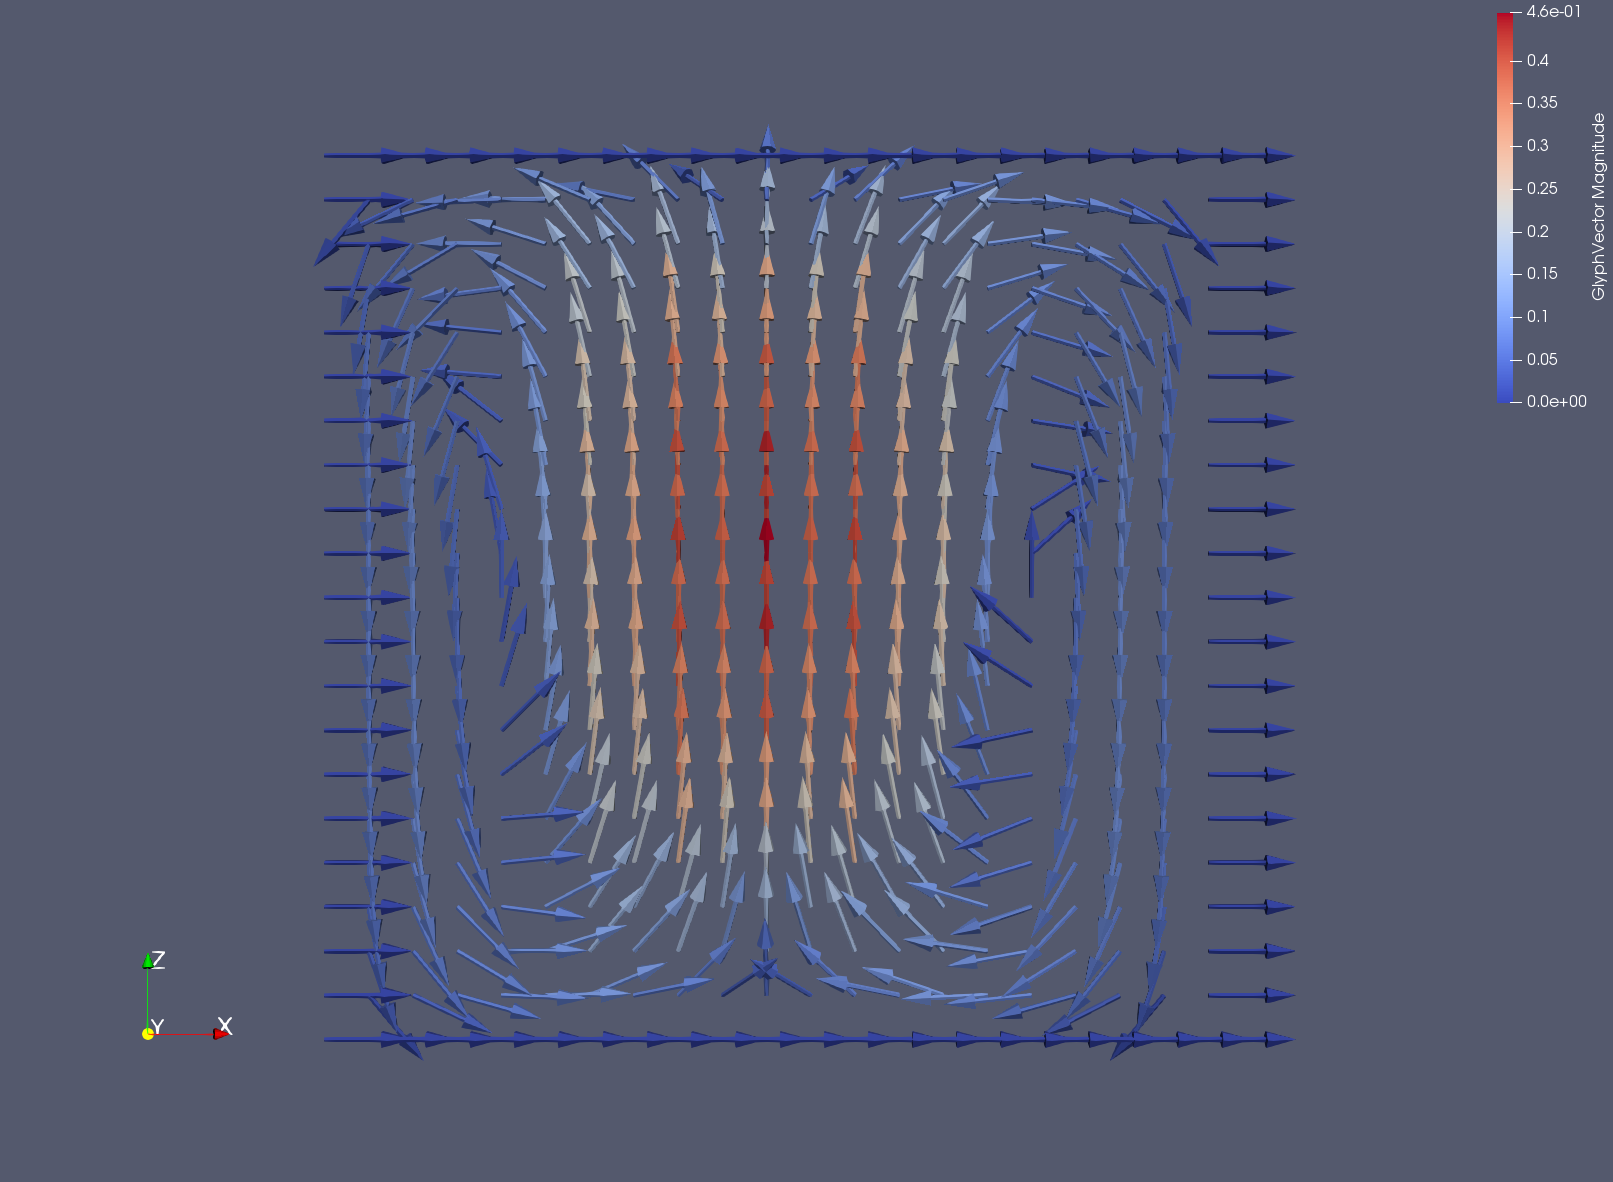
\includegraphics[height = 8cm, keepaspectratio]{graphes/Paraview/coupe_aimant_centre.png} 
\caption{\label{figure 31 } coupe du champ de vitesse selon le plan XZ, pour Y petit (on est proche de l'aimant), Paraview}
\end{center}
\end{figure}



\begin{figure}[!h]
\begin{center}
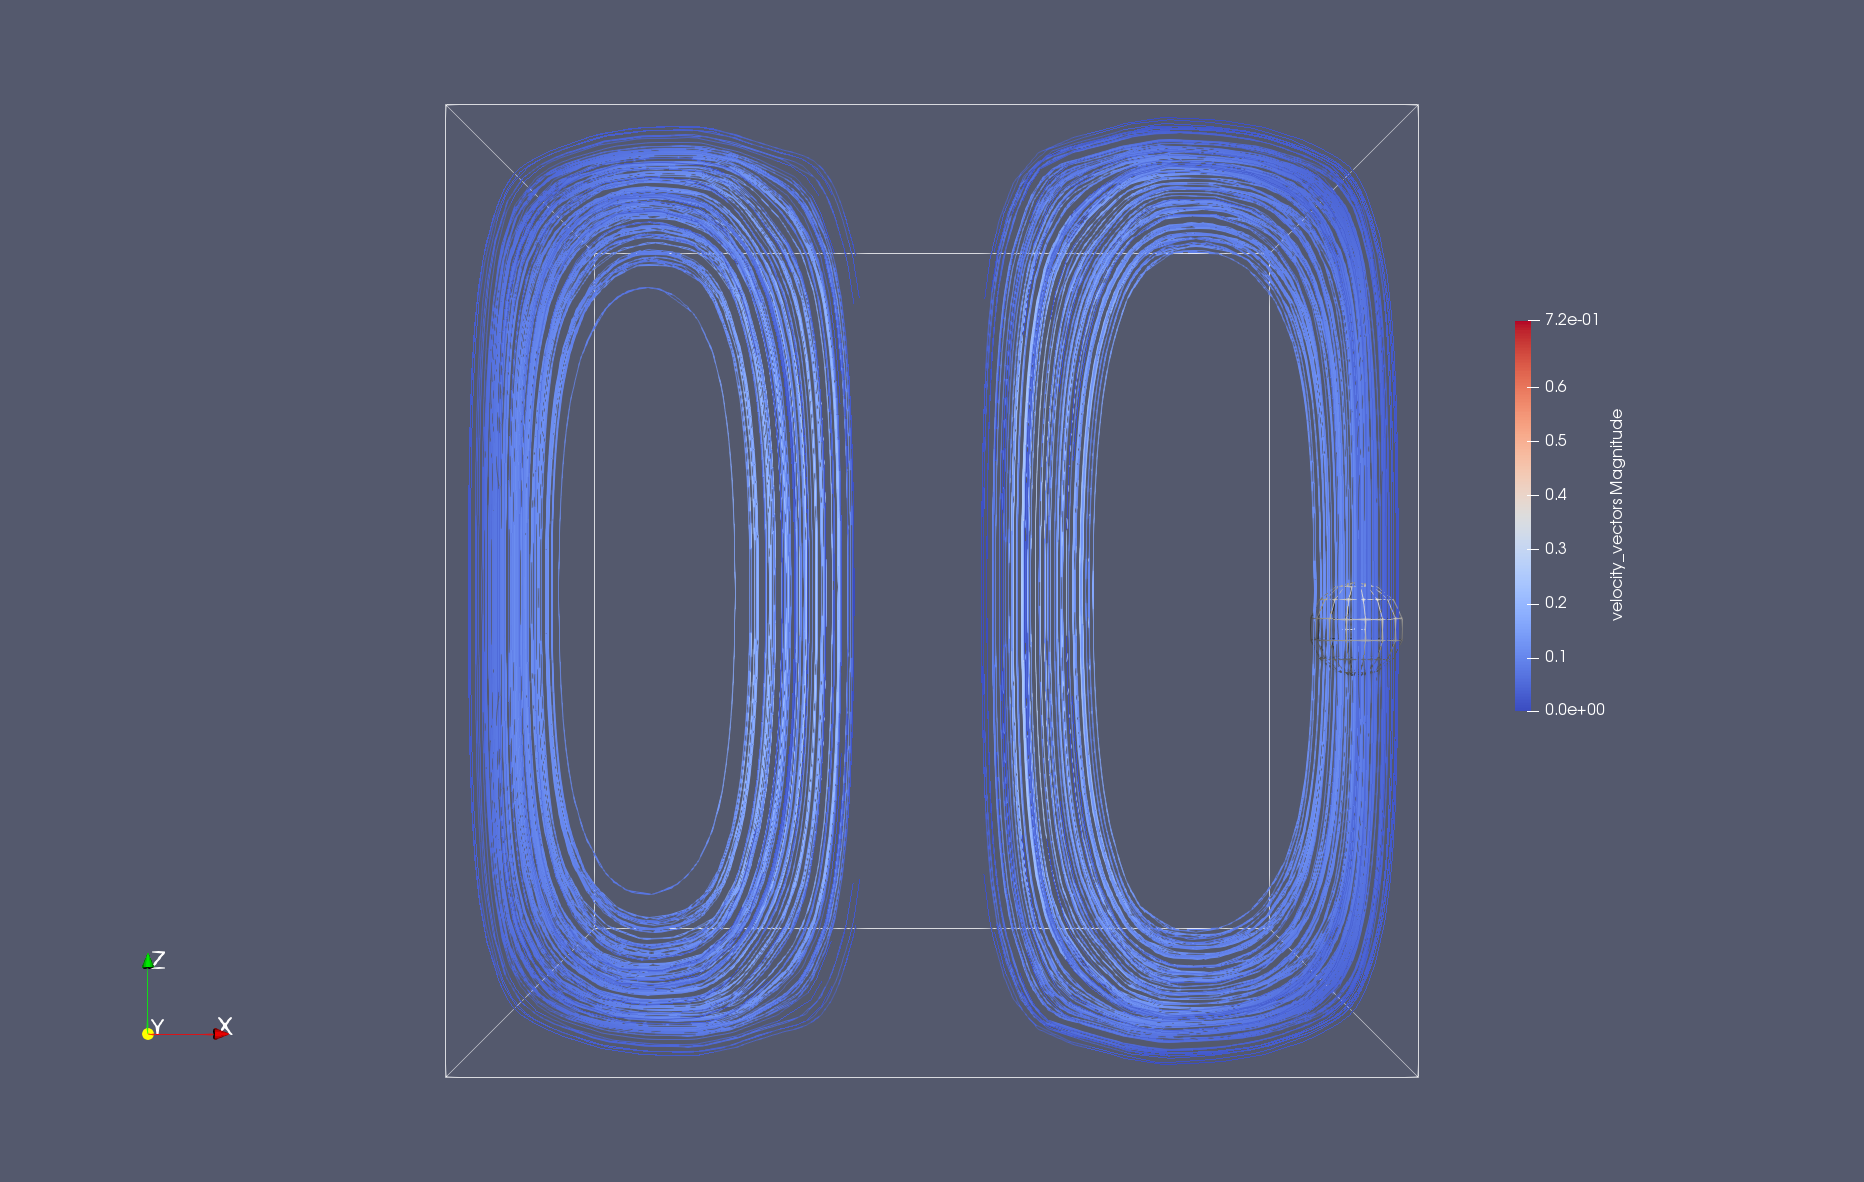
\includegraphics[height = 6cm, keepaspectratio]{graphes/Paraview/flux_aimant_centre_100pt_length4.png} 
\caption{\label{figure 32 }2 flux de particules dans cuve pour l'aimant centré pour des sphères de rayon 0.05 contenant 100 particules et pour un $max$ $StreamLine$ $FLux$ de 3, Paraview}
\end{center}
\end{figure}

A présent que nous avons observé de beaux tourbillons près de l'aimant, nous pouvons nous intéresser à ce qui se passe sur les tourbillons au fur et à mesure que l'on s'en éloigne, et voir ainis les conséquences de l'hypothèse d'un champ magnétique uniforme. 

\begin{figure}[!h]
\begin{center}
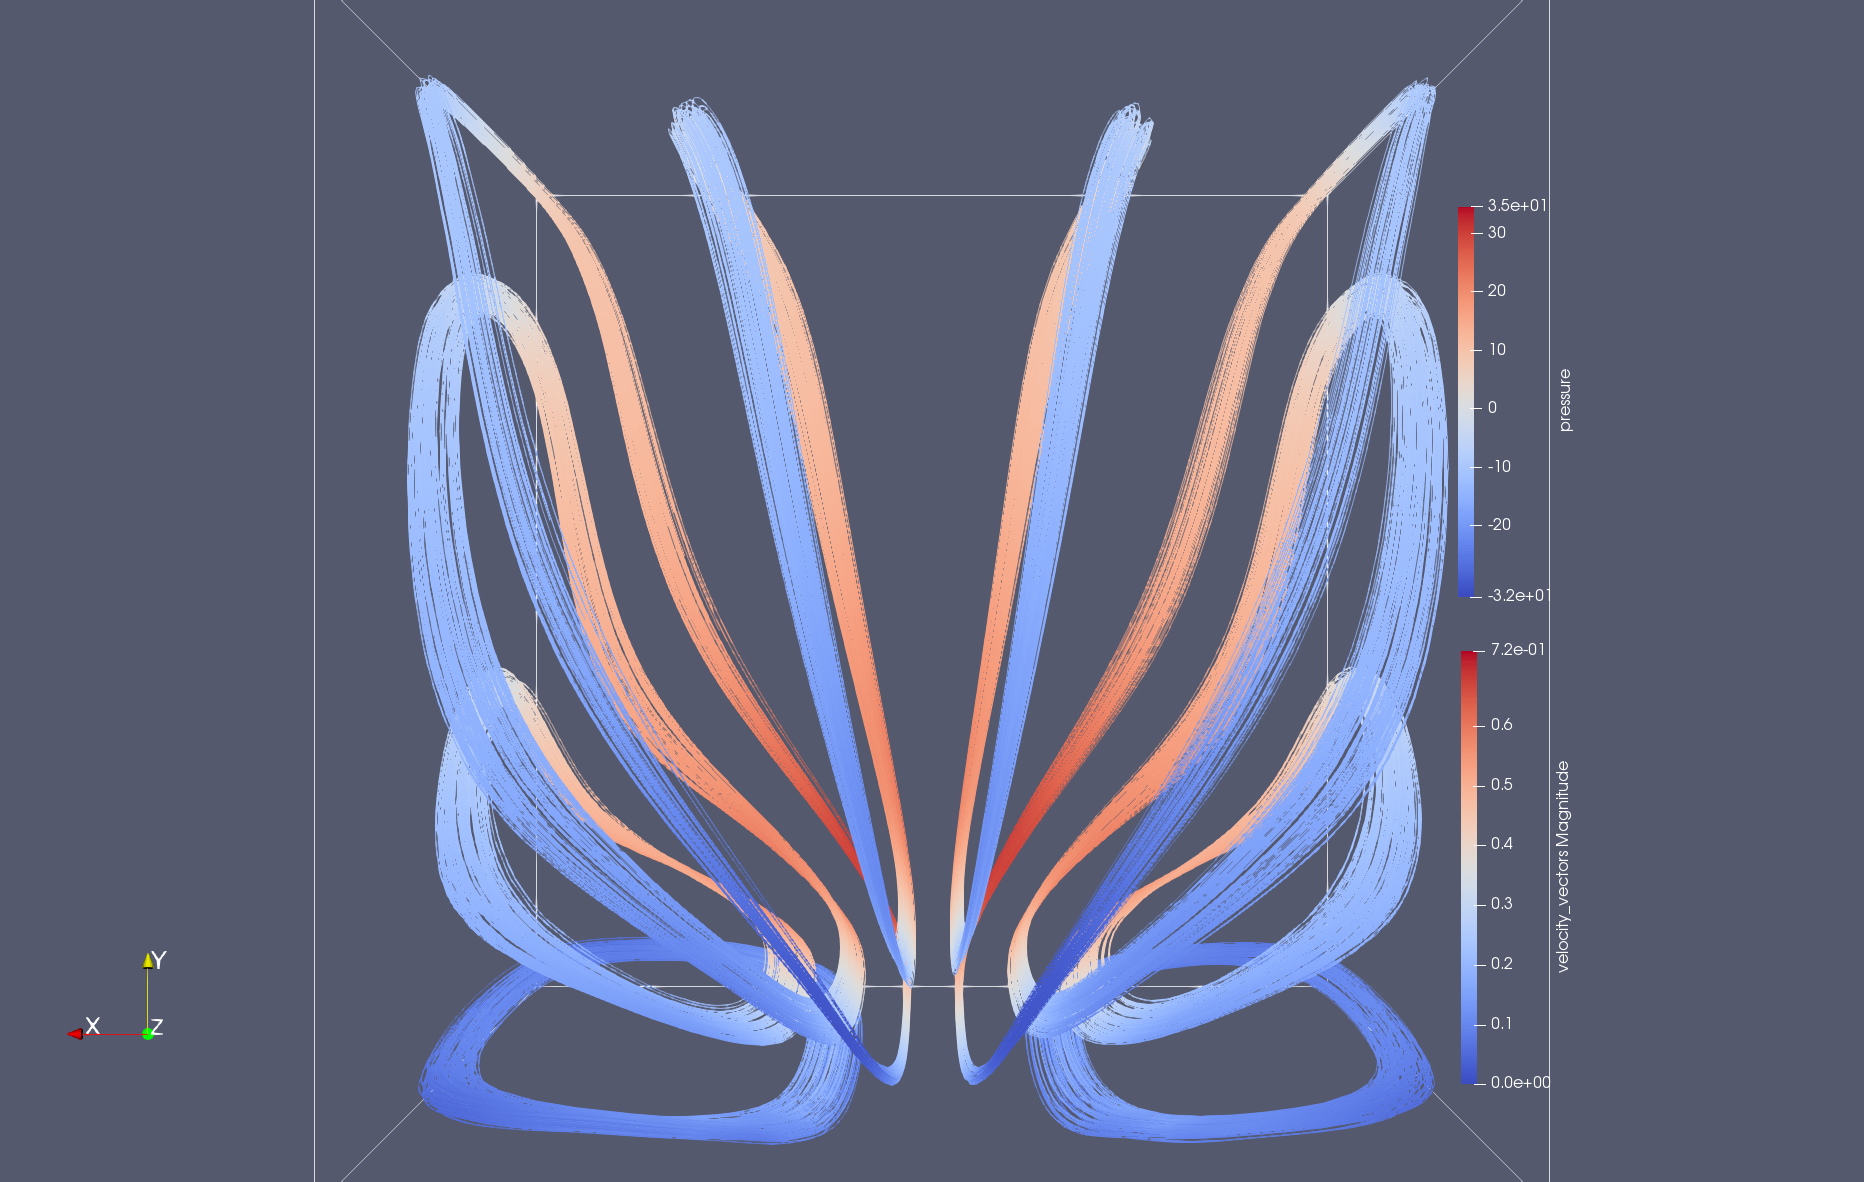
\includegraphics[height = 8cm, keepaspectratio]{graphes/Paraview/differents_flux_centre_100pt_lenght4_rad05.png} 
\caption{\label{figure 33}différents flux dans le plan XY pour des sphères de rayon 0.02 contenant 100 particules et pour un max $StreamLine$ $FLux$ de 3, avec un aimant centré, Paraview}
\end{center}
\end{figure}

Nous pouvons comparer à la coupe sur le plan XY du champ magnétique pour cette configuration.

\begin{figure}[!h]
\begin{center} 
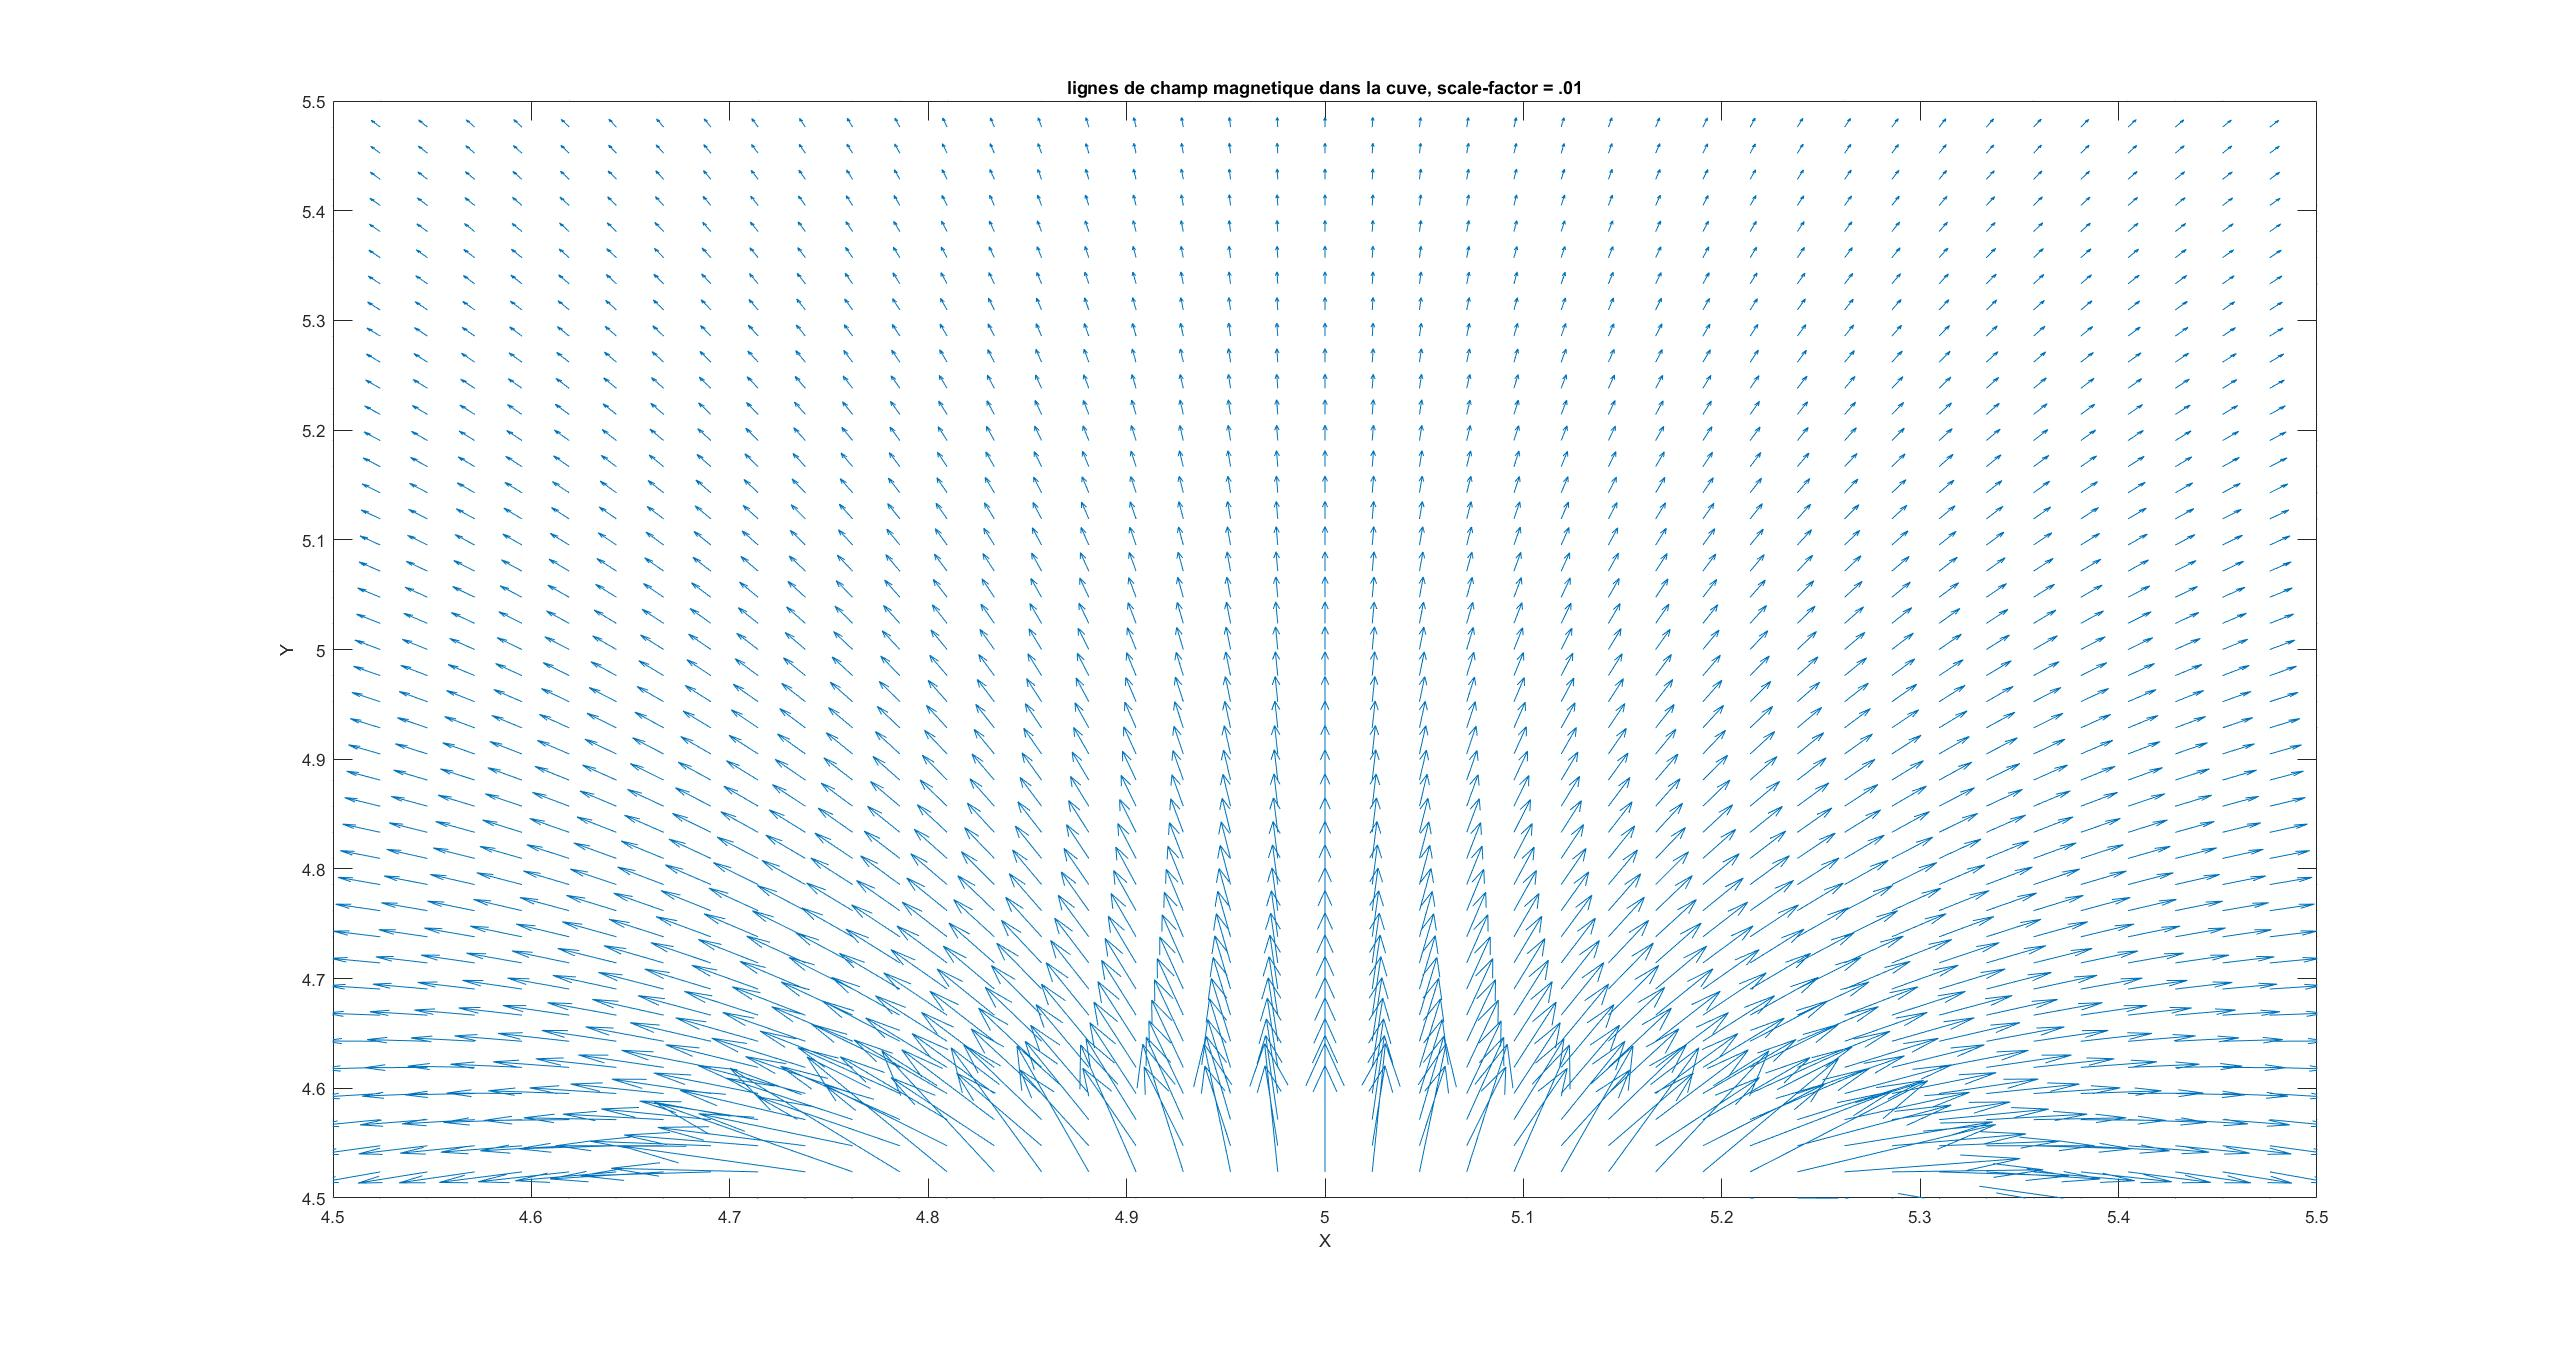
\includegraphics[height = 8cm, keepaspectratio]{graphes/coupe_2D_champ_centre.jpg} 
\caption{\label{figure 34} champ magnétique selon XY avec un aimant centré}
\end{center}
\end{figure}
Nous apercevons sur la figure \ref{figure 34} que la déformation du tourbillon suit les lignes de champ magnétique, avec un module de vitesse constant sur les lignes de champ, ce qui est logique comme la force magnétique est constante sur les lignes de champ.\\

\begin{figure}[!h]
\begin{center} 
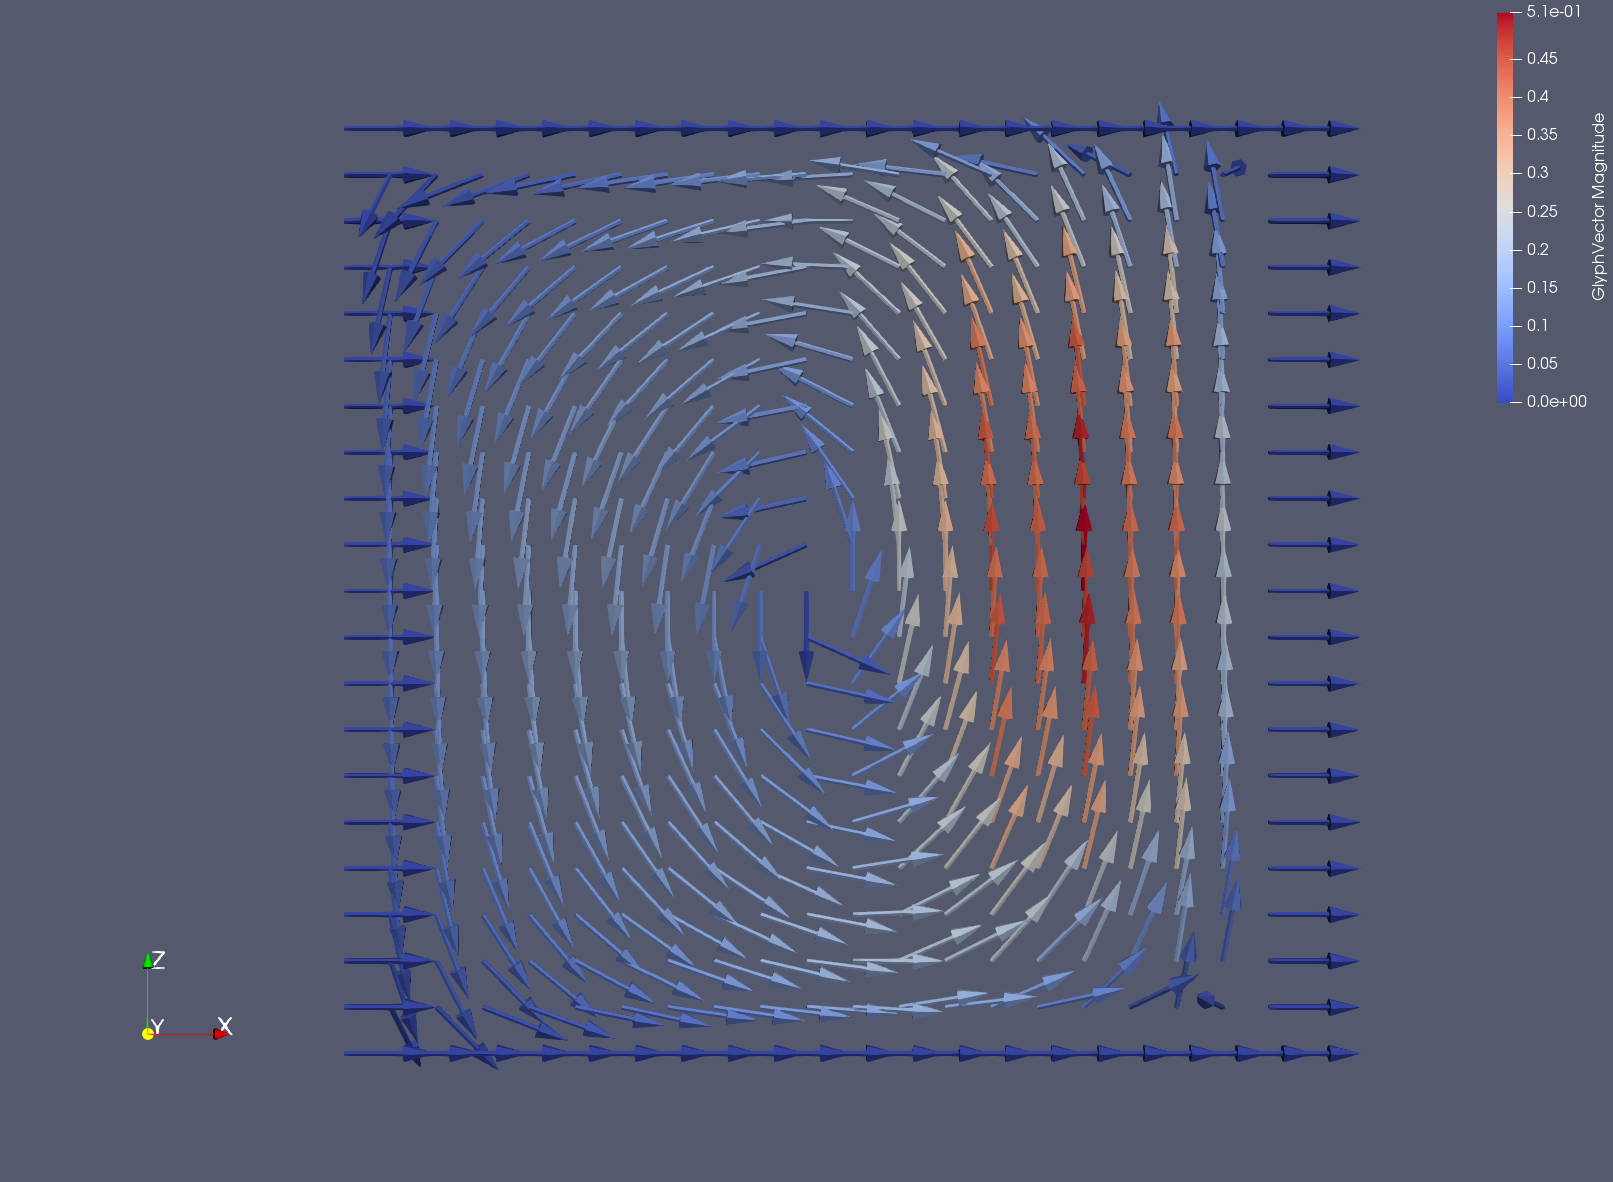
\includegraphics[height = 8cm, keepaspectratio]{graphes/Paraview/coupe_aimant_decentre.png} 
\caption{\label{figure 35}coupe du champ de vitesse selon le plan XZ, pour Y petit (on est proche de l'aimant)}
\end{center}
\end{figure}


\begin{figure}[!h]
\begin{center} 
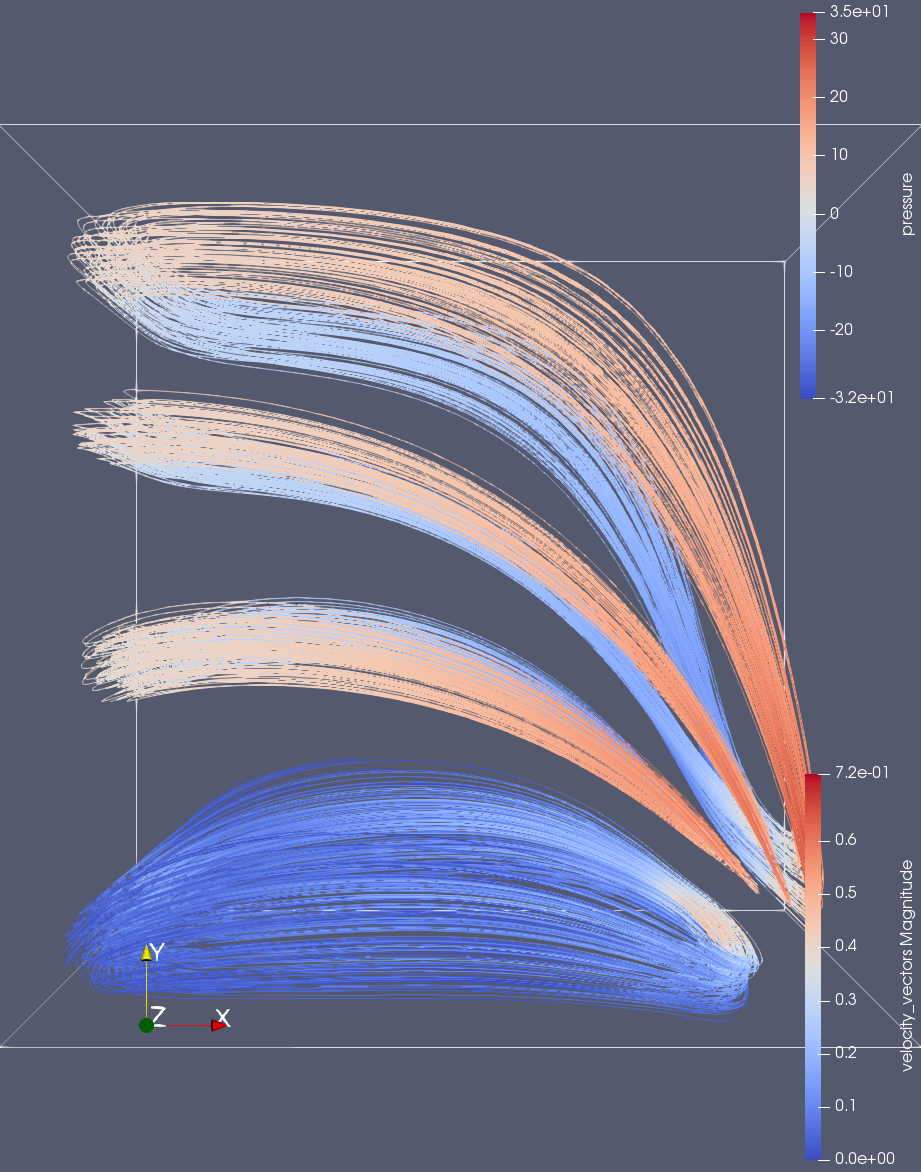
\includegraphics[height = 10cm, keepaspectratio]{graphes/Paraview/differents_flux_decentre_100pt_lenght4_rad05.png} 
\caption{\label{figure 36 }  différents flux pour un aimant centré utilisation de $StreamTracer$pour des sphères de rayon 0.05 contenant 100 particules et pour un max $StreamLine$ $FLux$ de 3}
\end{center}
\end{figure}

Ensuite de même pour l'aimant décentré (avant la transposition du champ de vitesse) on observe
sur le plan de coupe près de l'aimant décentré un tourbillon centré selon z dans la cuve, et les observations des flux de particules montrent que le tourbillon suit la forme des lignes de champs. \\



\begin{figure}[!h]
\begin{center}
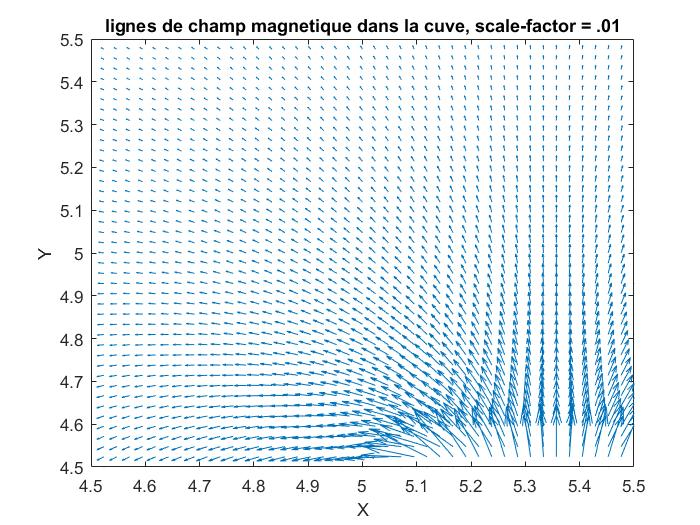
\includegraphics[height = 8cm, keepaspectratio]{graphes/coupe_2D_champ_decentre.jpg} 
\caption{\label{figure 39 } champ magnétique selon XY avec un aimant centré}
\end{center}
\end{figure}

\newpage
Enfin pour le champ de vitesse qui est la sommes des deux précedents nous observons les champ de vitesses sur les coupes 2D selon YZ, et XZ proches des aimants.  On voit que proche des aimants les tourbillons sont peut perturbés (Ici le rapport nentre les forces magnétiques pour les deux forces est 1).
\newpage
\begin{figure}[!h]
\center 
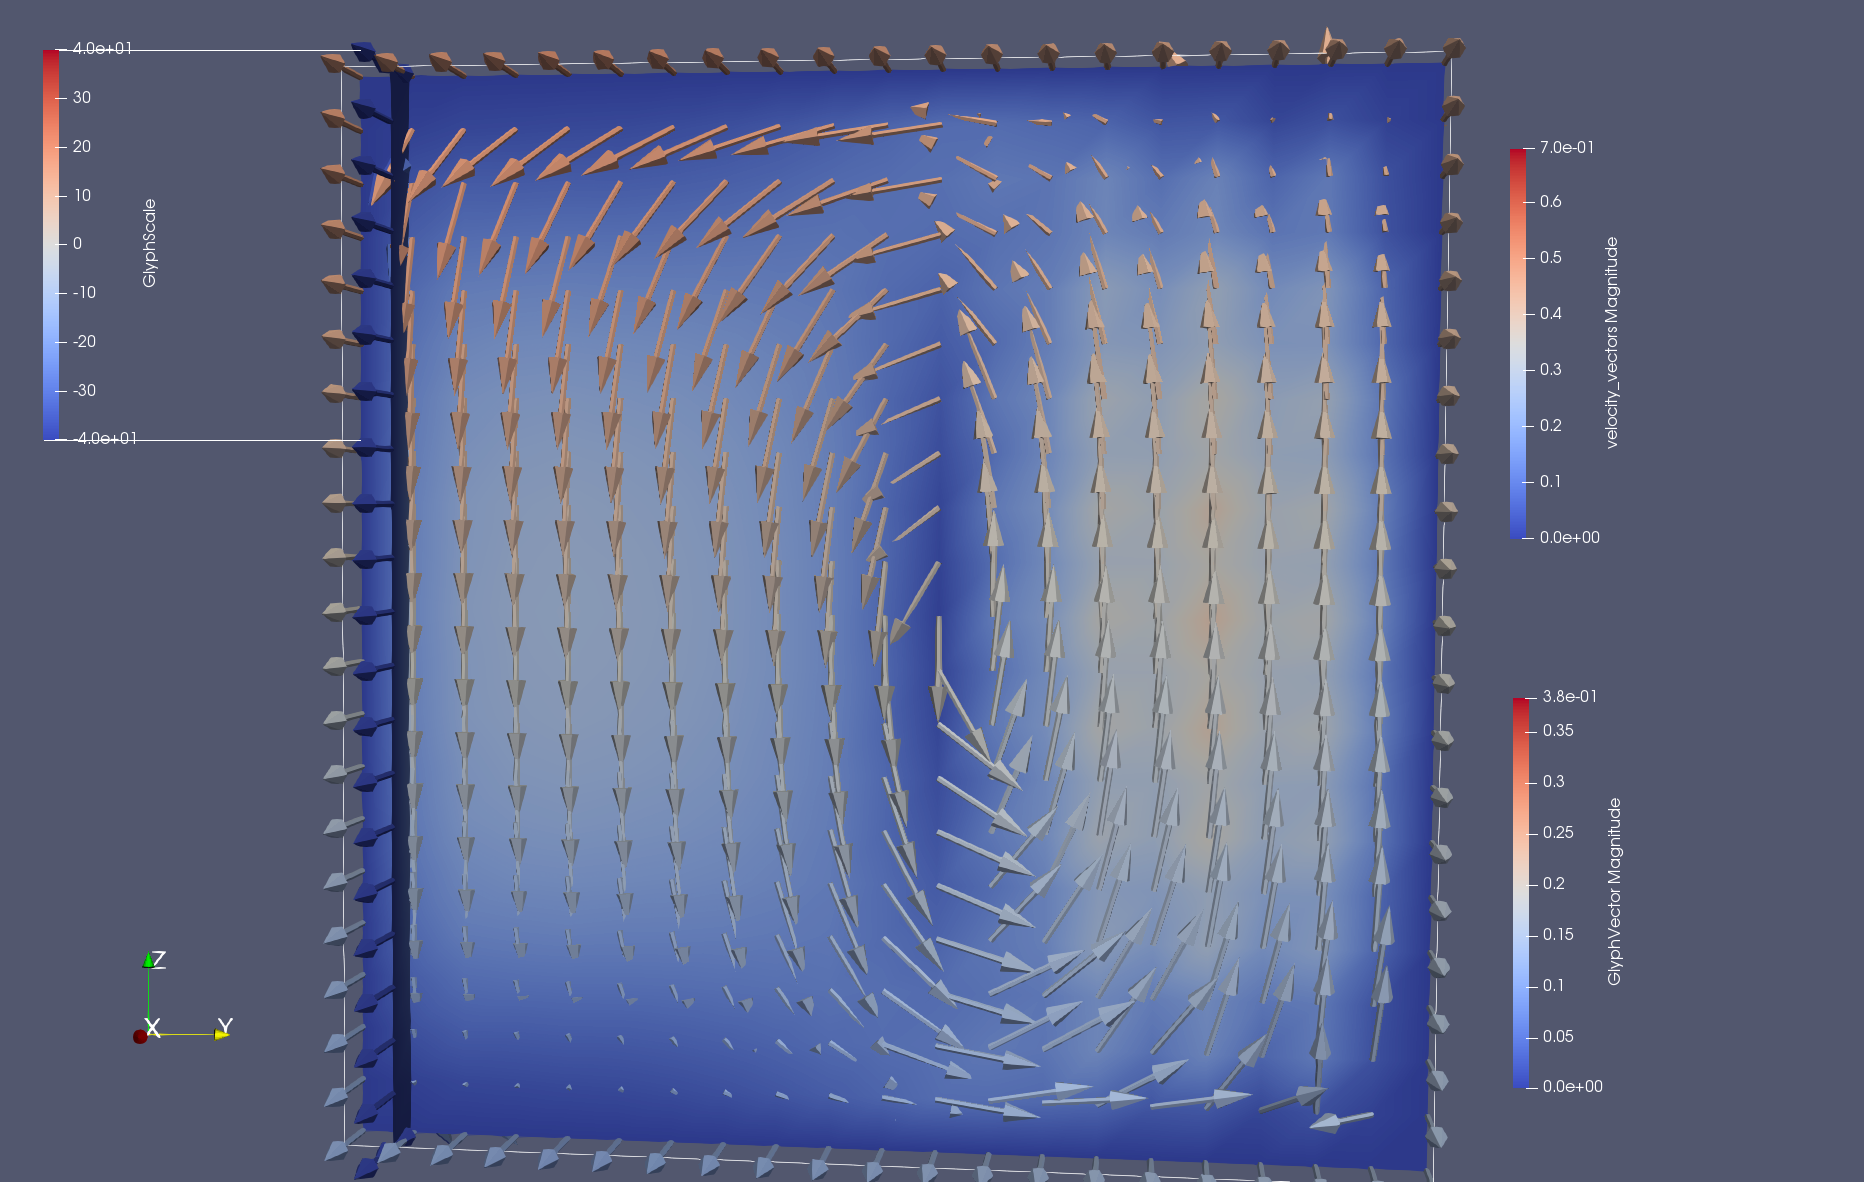
\includegraphics[height = 8cm, keepaspectratio]{graphes/Paraview/total_coupe_pret_aimant_decentre.png} 
\caption{\label{figure 322 } coupe selon YZ, proche de l'aimant pour le champ de vitesse complet}
\end{figure}

\begin{figure}[!h]
\center 
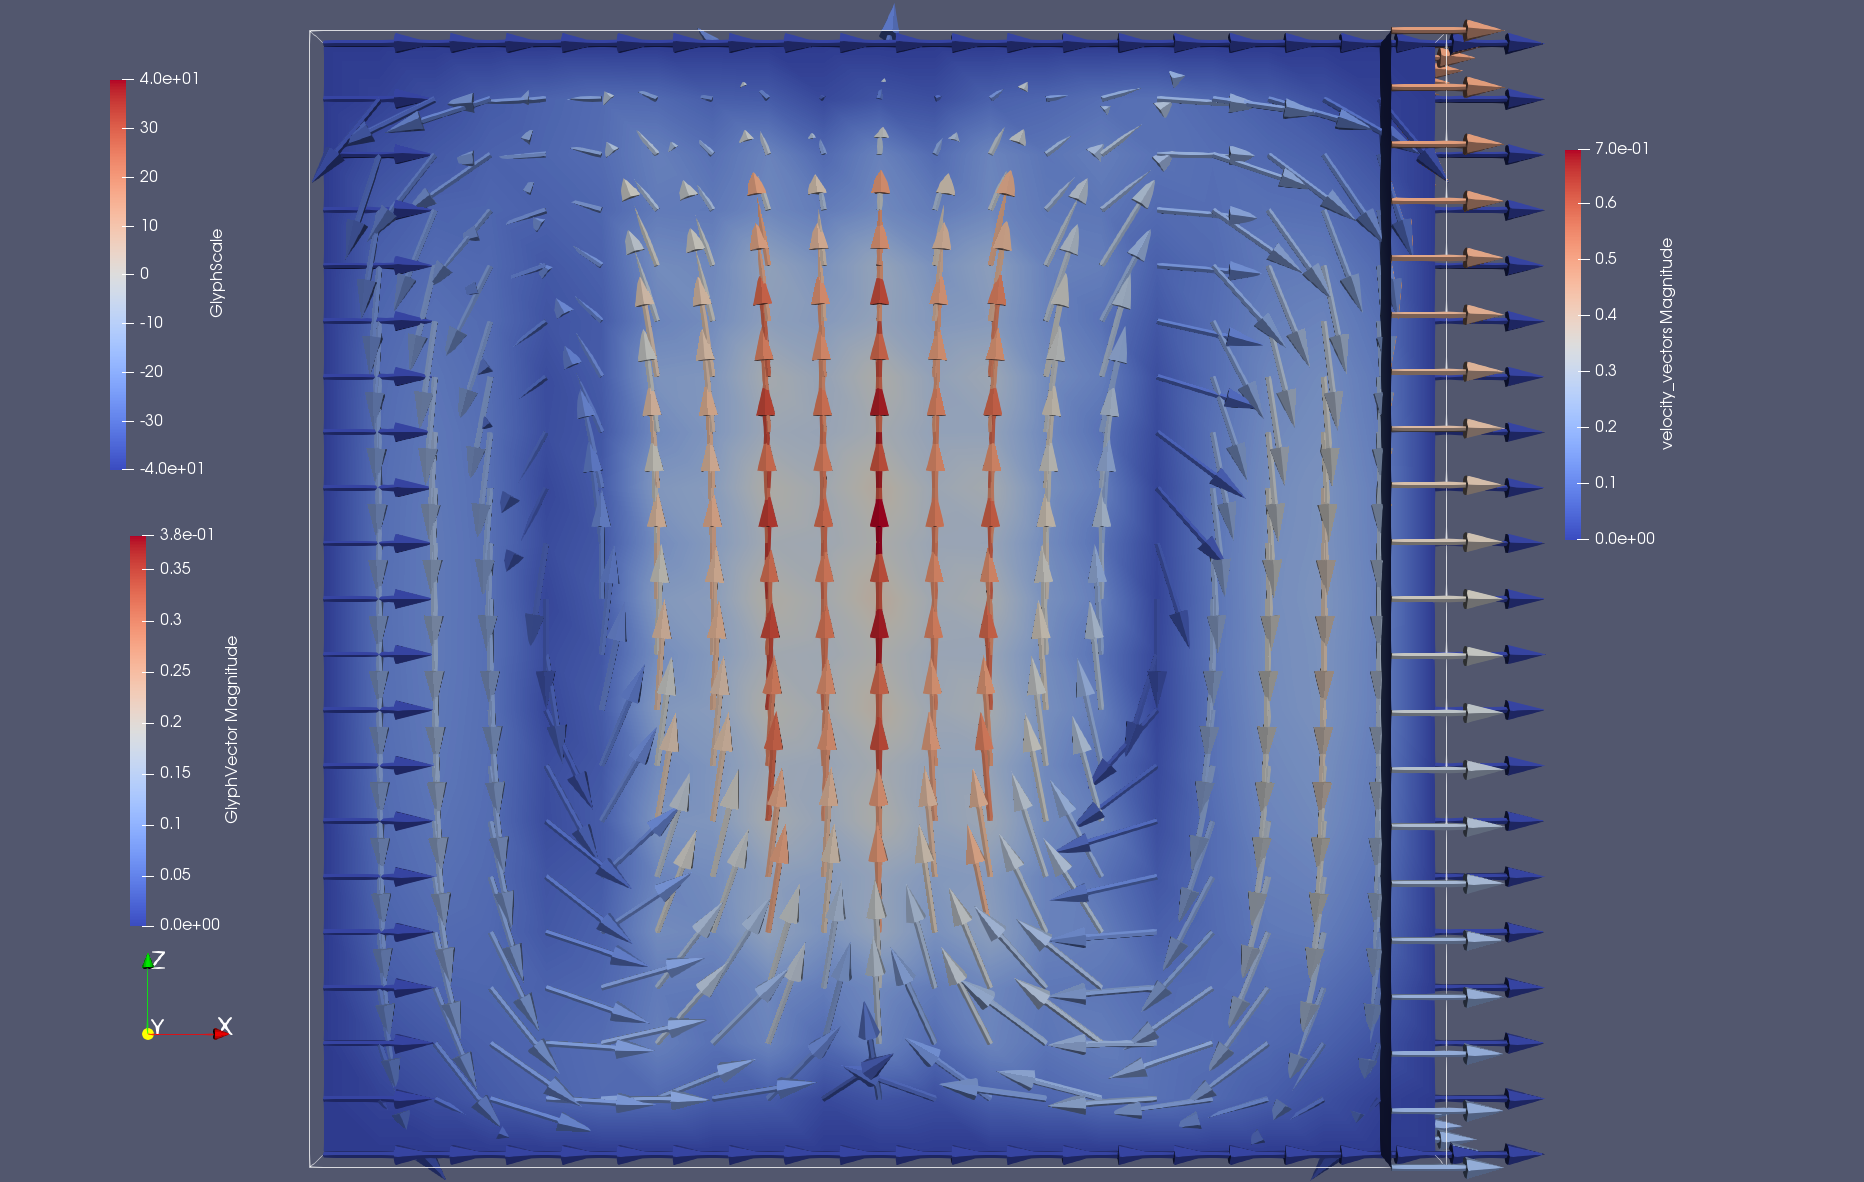
\includegraphics[height = 8cm, keepaspectratio]{graphes/Paraview/total_coupe_pret_aimant_centre.png} 
\caption{\label{figure 3 } coupe selon XZ, proche de l'aimant pour le champ de vitesse complet}
\end{figure}

\begin{figure}[!h]
\center 
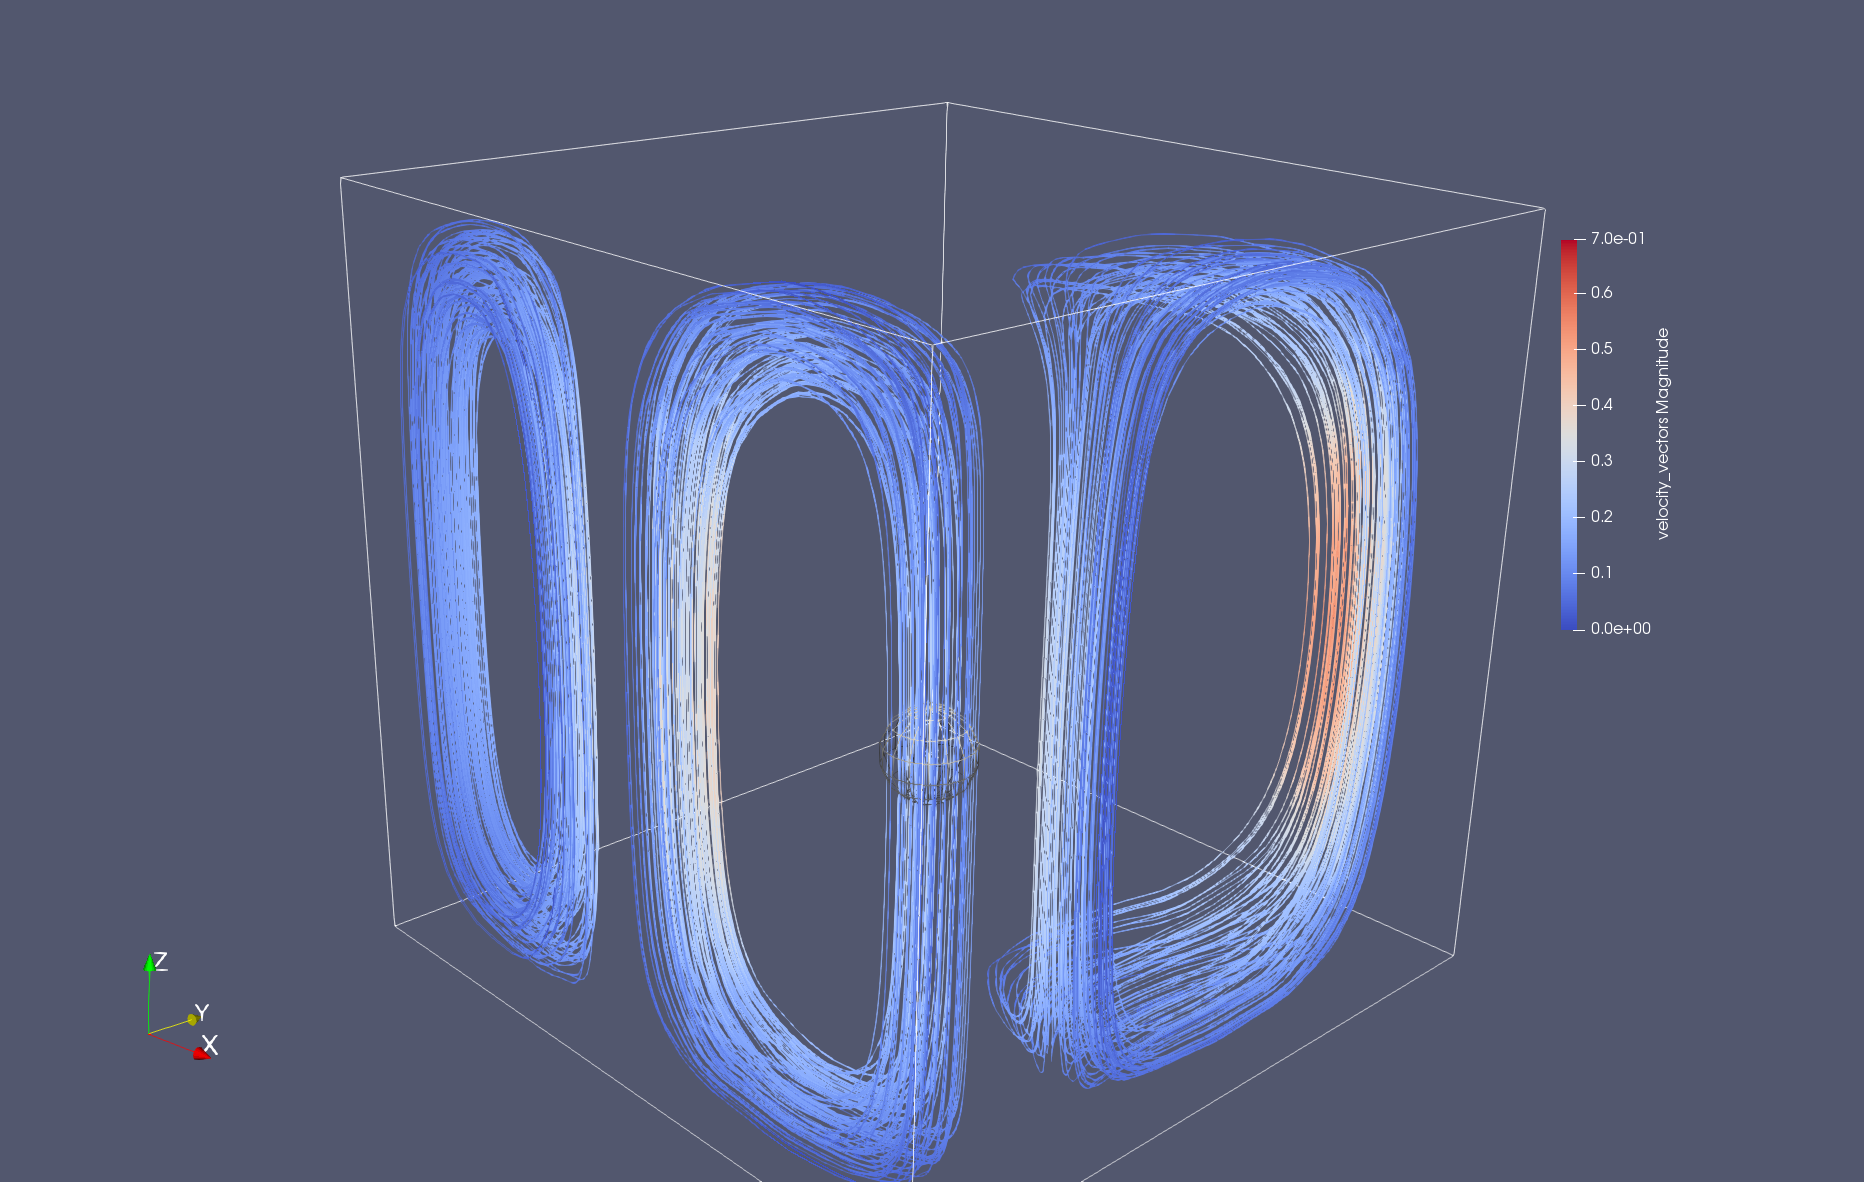
\includegraphics[height = 8cm, keepaspectratio]{graphes/Paraview/total_3_flux.png} 
\caption{\label{figure 3 }trois flus de particules près des aimants pour le champ de vitesse total}
\end{figure}

%================== sections de Poincarré ==========================================================
\newpage

\subsection{Les sections de Poincaré}
Pour caractériser les propriétés chaotiques des trajectoires associées à ce champ de vitesse, nous allons utiliser l'outil classique de la théorie des systèmes dynamiques qu'est la section de Poincaré, dont l'un des atouts est qu'elle permet de diminuer la complexité des problèmes par une réduction du nombre de dimensions. 
\\
En mathématiques, particulièrement en système dynamique, une application de Poincaré est une application liée à une orbite périodique dans l’espace des états d’un système dynamique et un certain sous-espace de dimension moindre, appelé la section de Poincaré, transverse au  flot système.\\
 Plus précisément, on considère une orbite suffisamment proche d'une orbite périodique, avec une condition initiale sur la section de Poincaré, et on observe le point auquel cette orbite revient à la section pour la première fois, d'où son autre nom, application de récurrence.
\\
En fait, les intersections successives avec S notées Pn d’une trajectoire donnée peuvent être vues comme les itérées d’une condition initiale P0 par une application de S dans S:
\\
\[f: P_n \in S \to P_{n+1} = f(P_n) \in S \]
\\
Dans notre cas, les sections introduites sont des hyperplans, qui coupent l'espace selon les coupes de courant qui nous intéresse, pour déterminer si advection chaotique il y a.
\\
En effet , l'équation d'évolution de la particule fluide est:
\\
\[ \frac{d\vec{x}}{dt} = \vec{U}(\vec{x}), \]
où $\vec{x}(t)$ est la position de la particule fluide à l'instant t, et $\vec{U}$ est le champ de la vitesse, qui est stationnaire ( ne dépend pas du temps) , donc l'espace des phases correspond à l'espace physique. 
\\
On a deux cas:
\\
-Sur la surface $\Sigma $ apparaît une courbe régulière, qui correspond à un tore de fluide , ou quelques points , qui correspondent à des orbites théorique. Étant donné qu'il y a rebouclement des particules sur une même trajectoire, on qualifie la zone de semi-régulière, et n'est donc pas efficace pour le mélange. 
\\

-En revanche, si l'ensemble des des intersections entre les trajectoires et l'hyperplan $\Sigma$ est disséminé sur une partie de la section $\Sigma$, on en conclut que la trajectoire a un comportement erratique, caractérisant une région chaotique, qui est du coup une région de bon mélange. 

%====================================================================================================
\subsection{A la recherche d'un écoulement chaotique}

En nous inspirant des travaux de Valérie Toussaint et du Travail accomplis l'annnée dernière sur le projet, nous allons reprendre le même principe et poser un rapport entre les deux force magnétique $\vec{f_1}$ qui donne un tourbillon et $\vec{f_2}$ qui donne deux tourbillons. Le but est 'd'équilibrer' les deux force pour avoir un mouvement d'advection chaotique à travers le paramètre dz contrôle R tel que :
\[ R = \frac{||\vec{f_1}||}{||\vec{f_2}||} \]

Nous allons donc exécuter au final le script $Resolution finale$ suivant pour résoudre notre problème en faisant varier R de telle manière à ensuite observer sur Paraview des sections de Poincaré permettant d'identifier des advections chaotiques.

\begin{verbatim}

%   résolution dans la configuration aimant centre
[X2,Y2,Z2,Uxgd_centre,Uygd_centre,Uzgd_centre,Pgd_centre] = stokes_3D(true,R);

%   résolution dans la configuration aimant de cote
[X2,Y2,Z2,Uxgd_cote,Uygd_cote,Uzgd_cote,Pgd_cote] = stokes_3D(false,R);

%   transposition du champ pour l'aimant décentré
[Uxgd_cote_transp,Uygd_cote_transp,Uzgd_cote_transp] = transposition_champ(Uxgd_cote,Uygd_cote,Uzgd_cote);


% prise en compte du rapport R, comme les équation sont linéaire cela revient à appliquer le 
% coefficient sur la vitesse.
R_i = norm(Uxgd_centre(:)) / norm(Uxgd_cote_transp(:));
Uxgd_cote_transp = (R / R_i) .* Uxgd_cote_transp;
Uxgd_total = Uxgd_centre + Uxgd_cote_transp;
Uygd_total = Uygd_centre + Uygd_cote_transp;
Uzgd_total = Uzgd_centre + Uzgd_cote_transp;
Pgd_total = Pgd_centre + Pgd_cote;

% sauvegarde au format .vtk pour Paraview
filename2_vtk='champ_de_vitesse_total_pour_R.vtk';
fprintf('   - au format VTK (''VTK STRUCTURED_GRID'') : %s\n',filename2_vtk);
writevtk3D(X2,Y2,Z2,Uxgd_total,Uygd_total,Uzgd_total,Pgd_total,filename2_vtk);
\end{verbatim}

Les sections de Poincarré que nous présentons se basent sur un maillage de la cuve en 21 points selon les trois directions de l'espace, et dans Paraview la simulation de la trajectoire de 100 000 particules (ce qui est le maximum compte-tenus de la RAM de la machine sur laquelle nous travaillons, nous pouvions éventuellement aller au-dessus mais le logiciel présentait alors des problèmes de stabilité), placée initialement dans une sphère centré sur la cuve de rayon 0.6 (qui occupe dons toute la cuve qui est un cube de coté 1). 
Nous utilisons la méthode d'interpolation définies par défaut : Runge Kutta 4-5 dans les deux directions d'intégration et avec un $Maximum$ $StreamLine$ $Length$ de 3. 

\begin{figure}[!h]
    \begin{minipage}[c]{.46\linewidth}
        \centering
        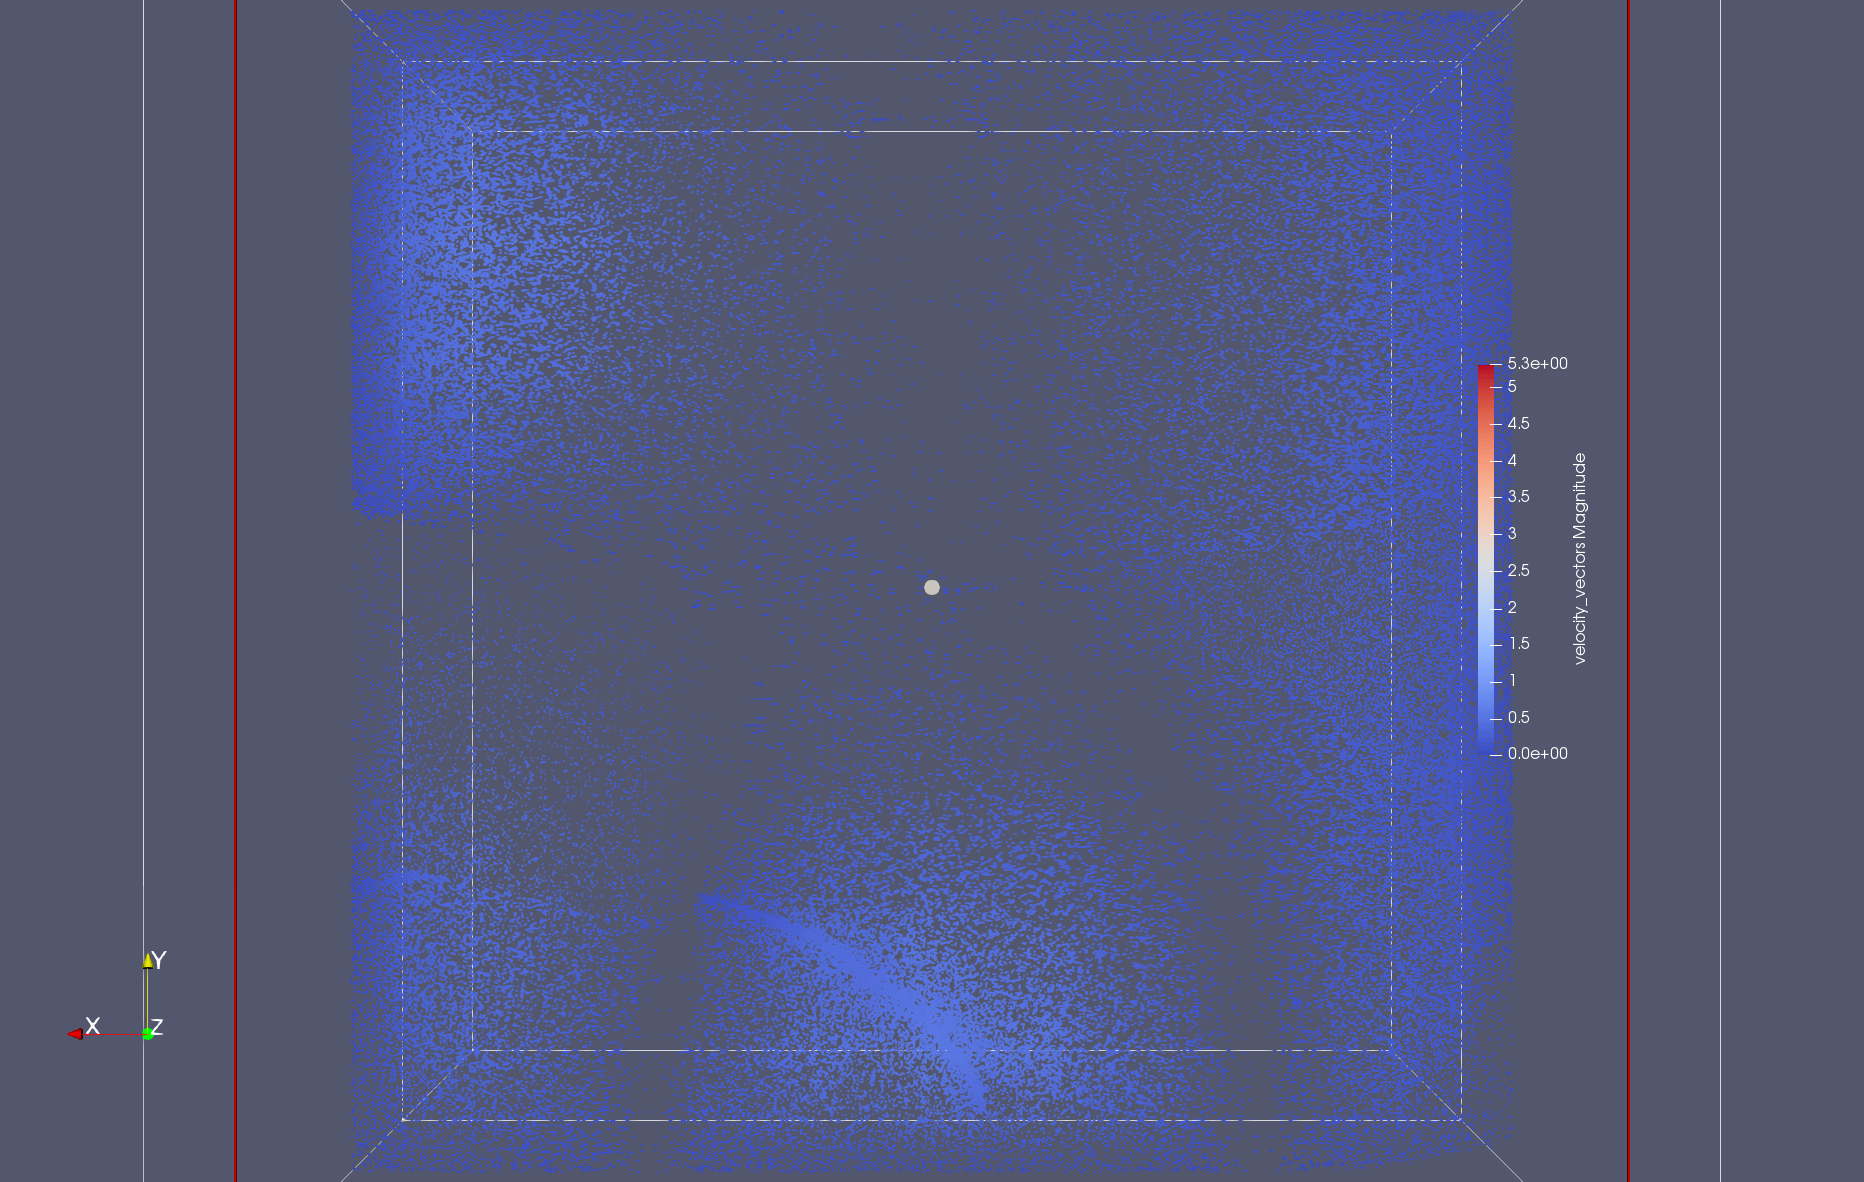
\includegraphics[height = 5cm, keepaspectratio]{graphes/Paraview/section_pioncarre_R_15.png}
        \caption{R = 15}
    \end{minipage}
    \hfill%
    \begin{minipage}[c]{.46\linewidth}
        \centering
        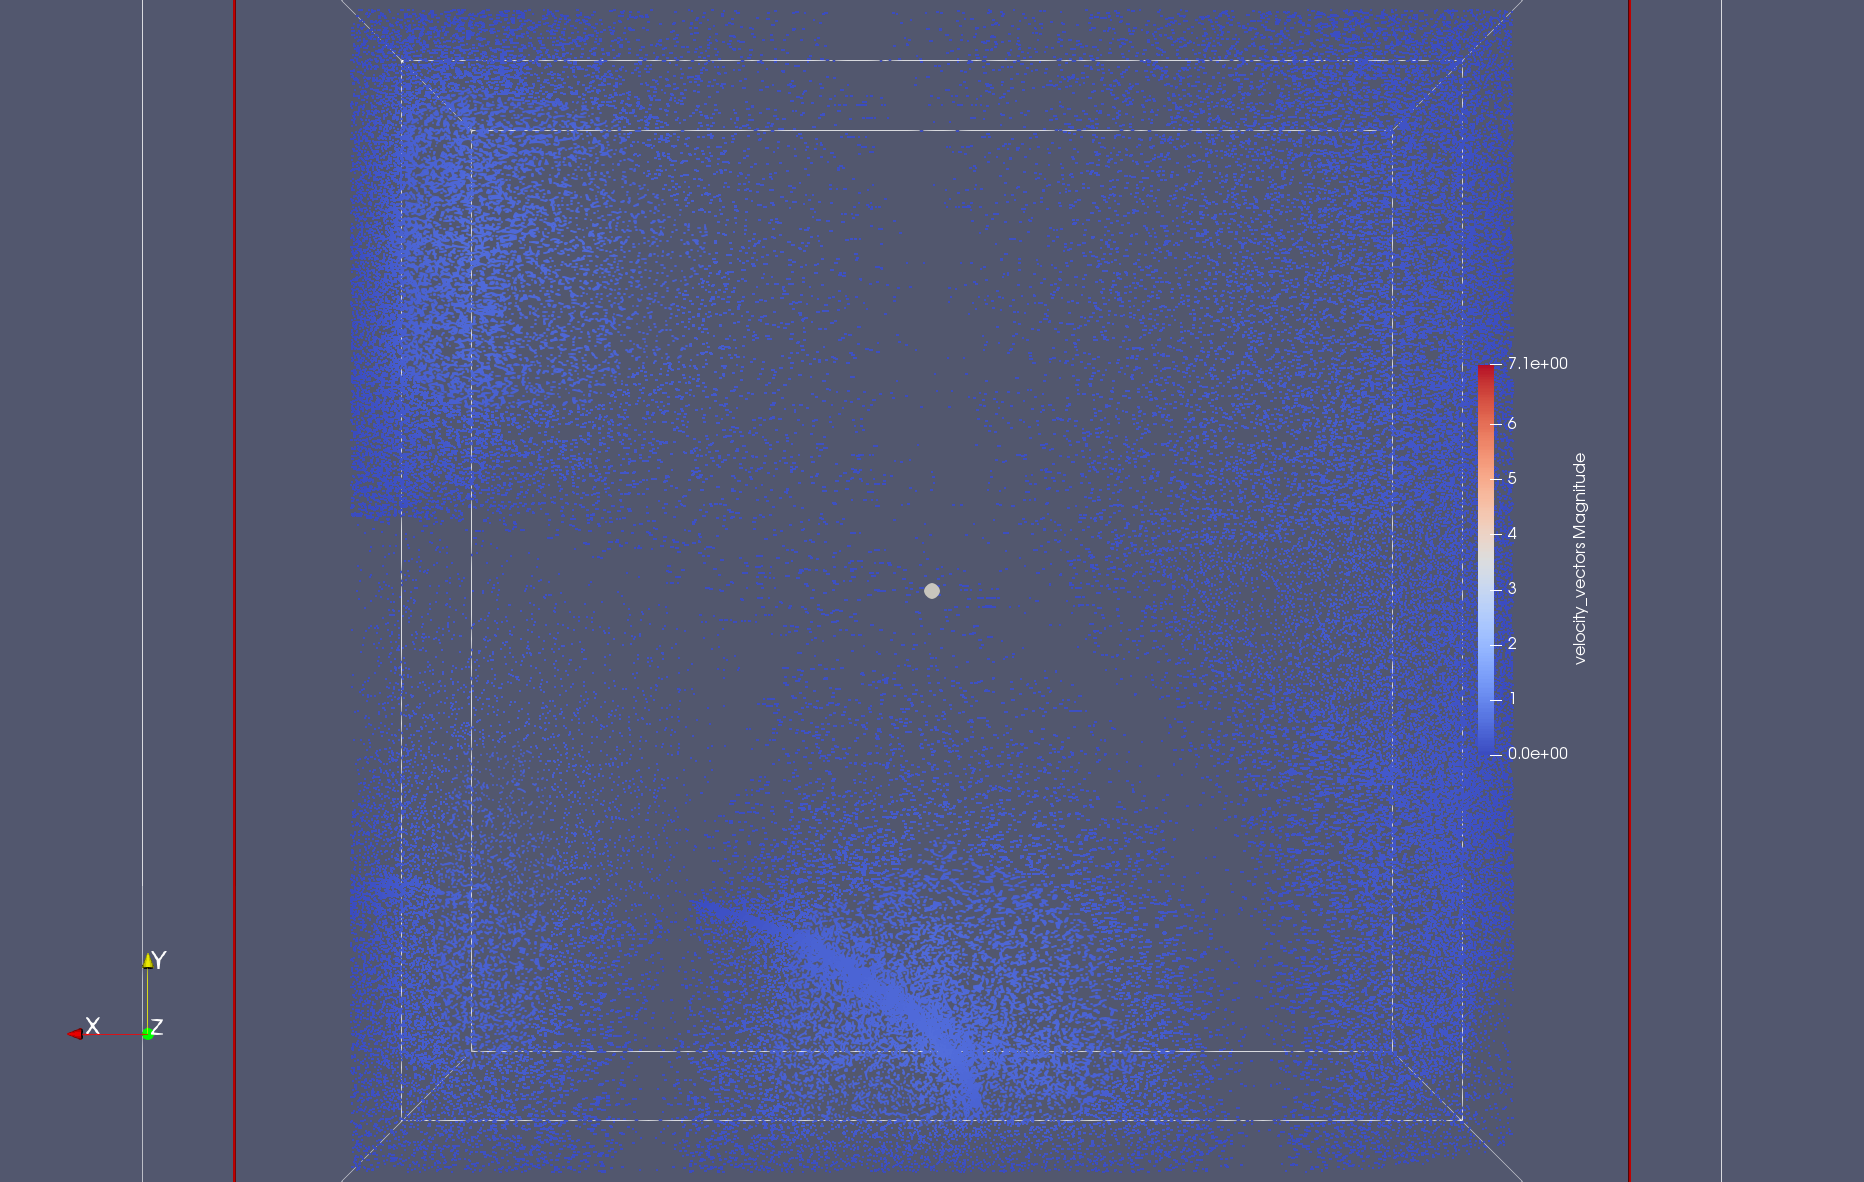
\includegraphics[height = 5cm, keepaspectratio]{graphes/Paraview/section_pioncarre_R_20.png}
        \caption{R = 20}
    \end{minipage}
\end{figure}
\begin{figure}[!h]
    \begin{minipage}[c]{.46\linewidth}
        \centering
        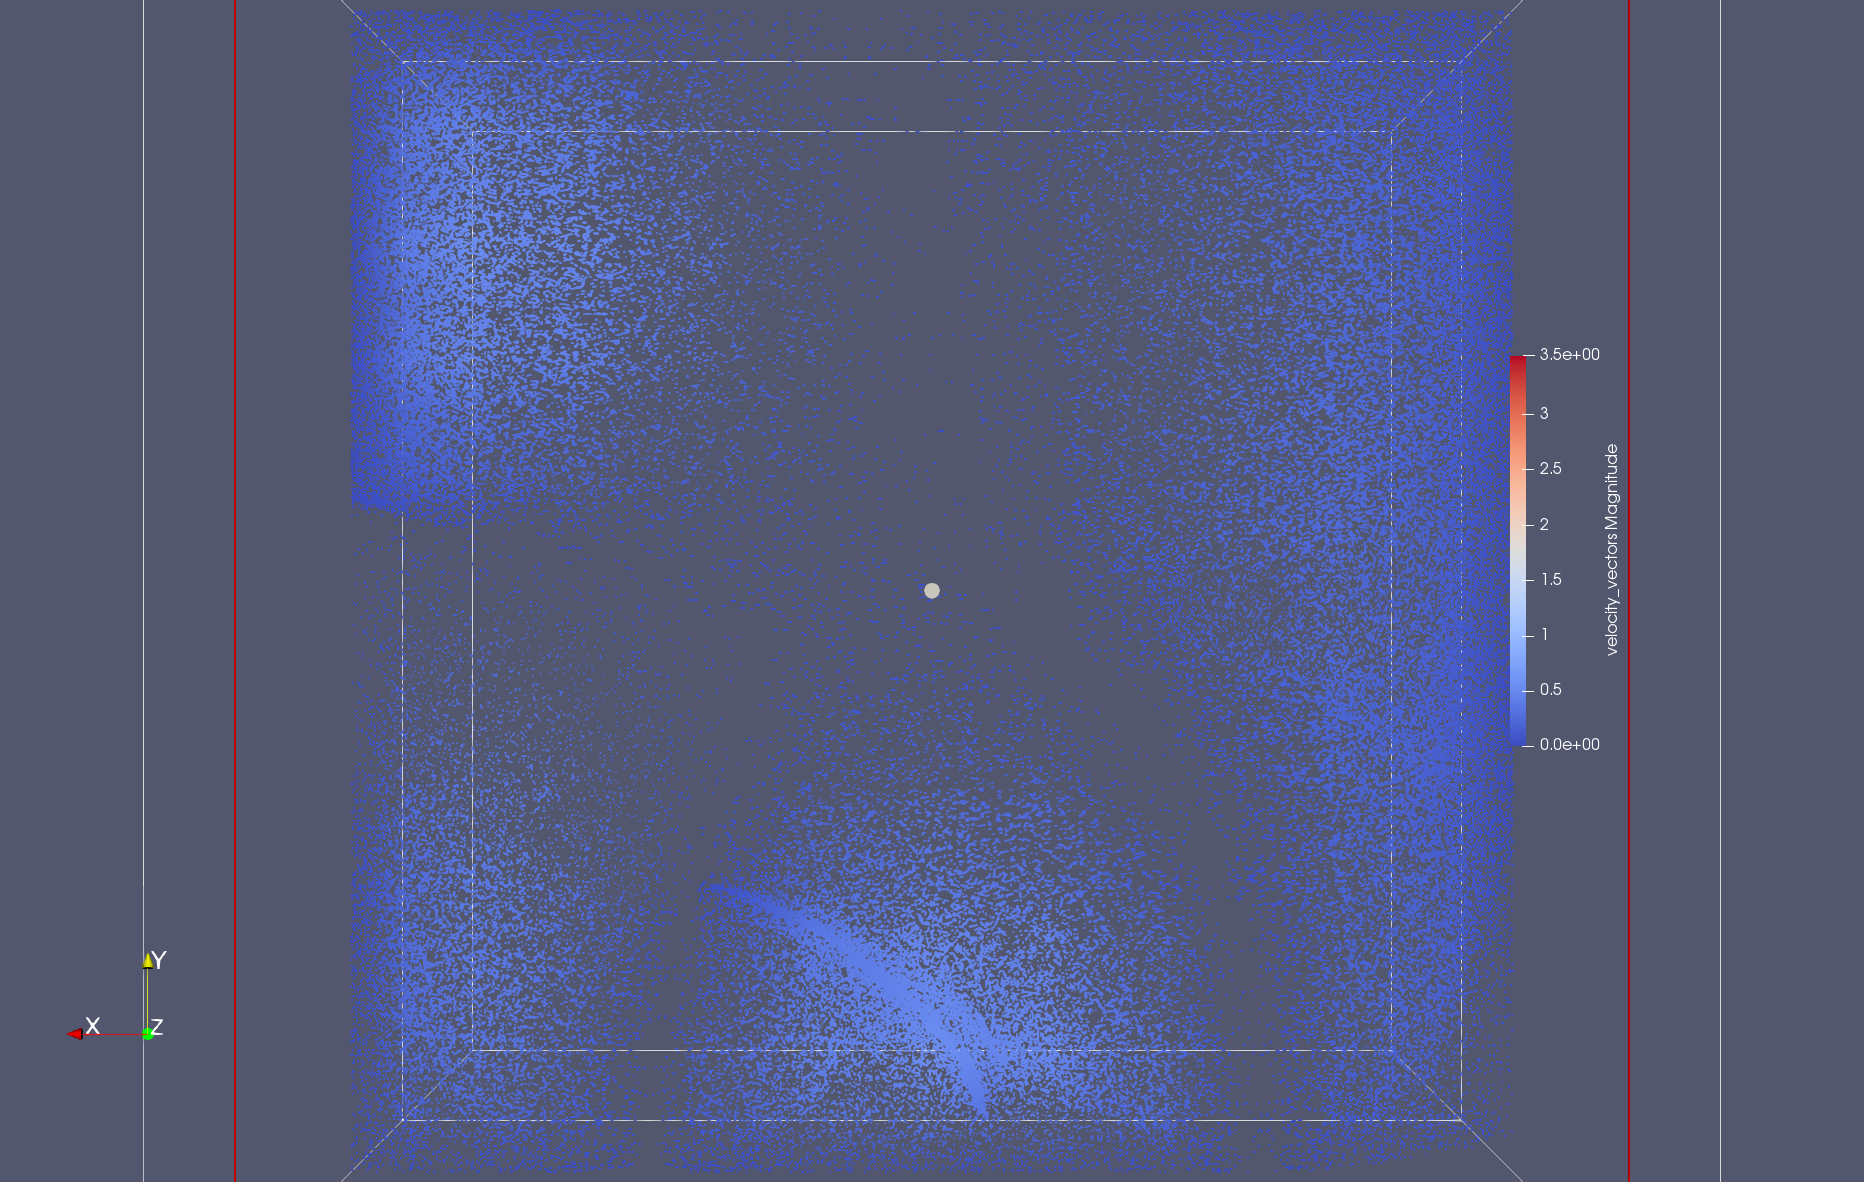
\includegraphics[height = 5cm, keepaspectratio]{graphes/Paraview/section_pioncarre_R_10.png}
        \caption{R = 10}
    \end{minipage}
    \hfill%
    \begin{minipage}[c]{.46\linewidth}
        \centering
        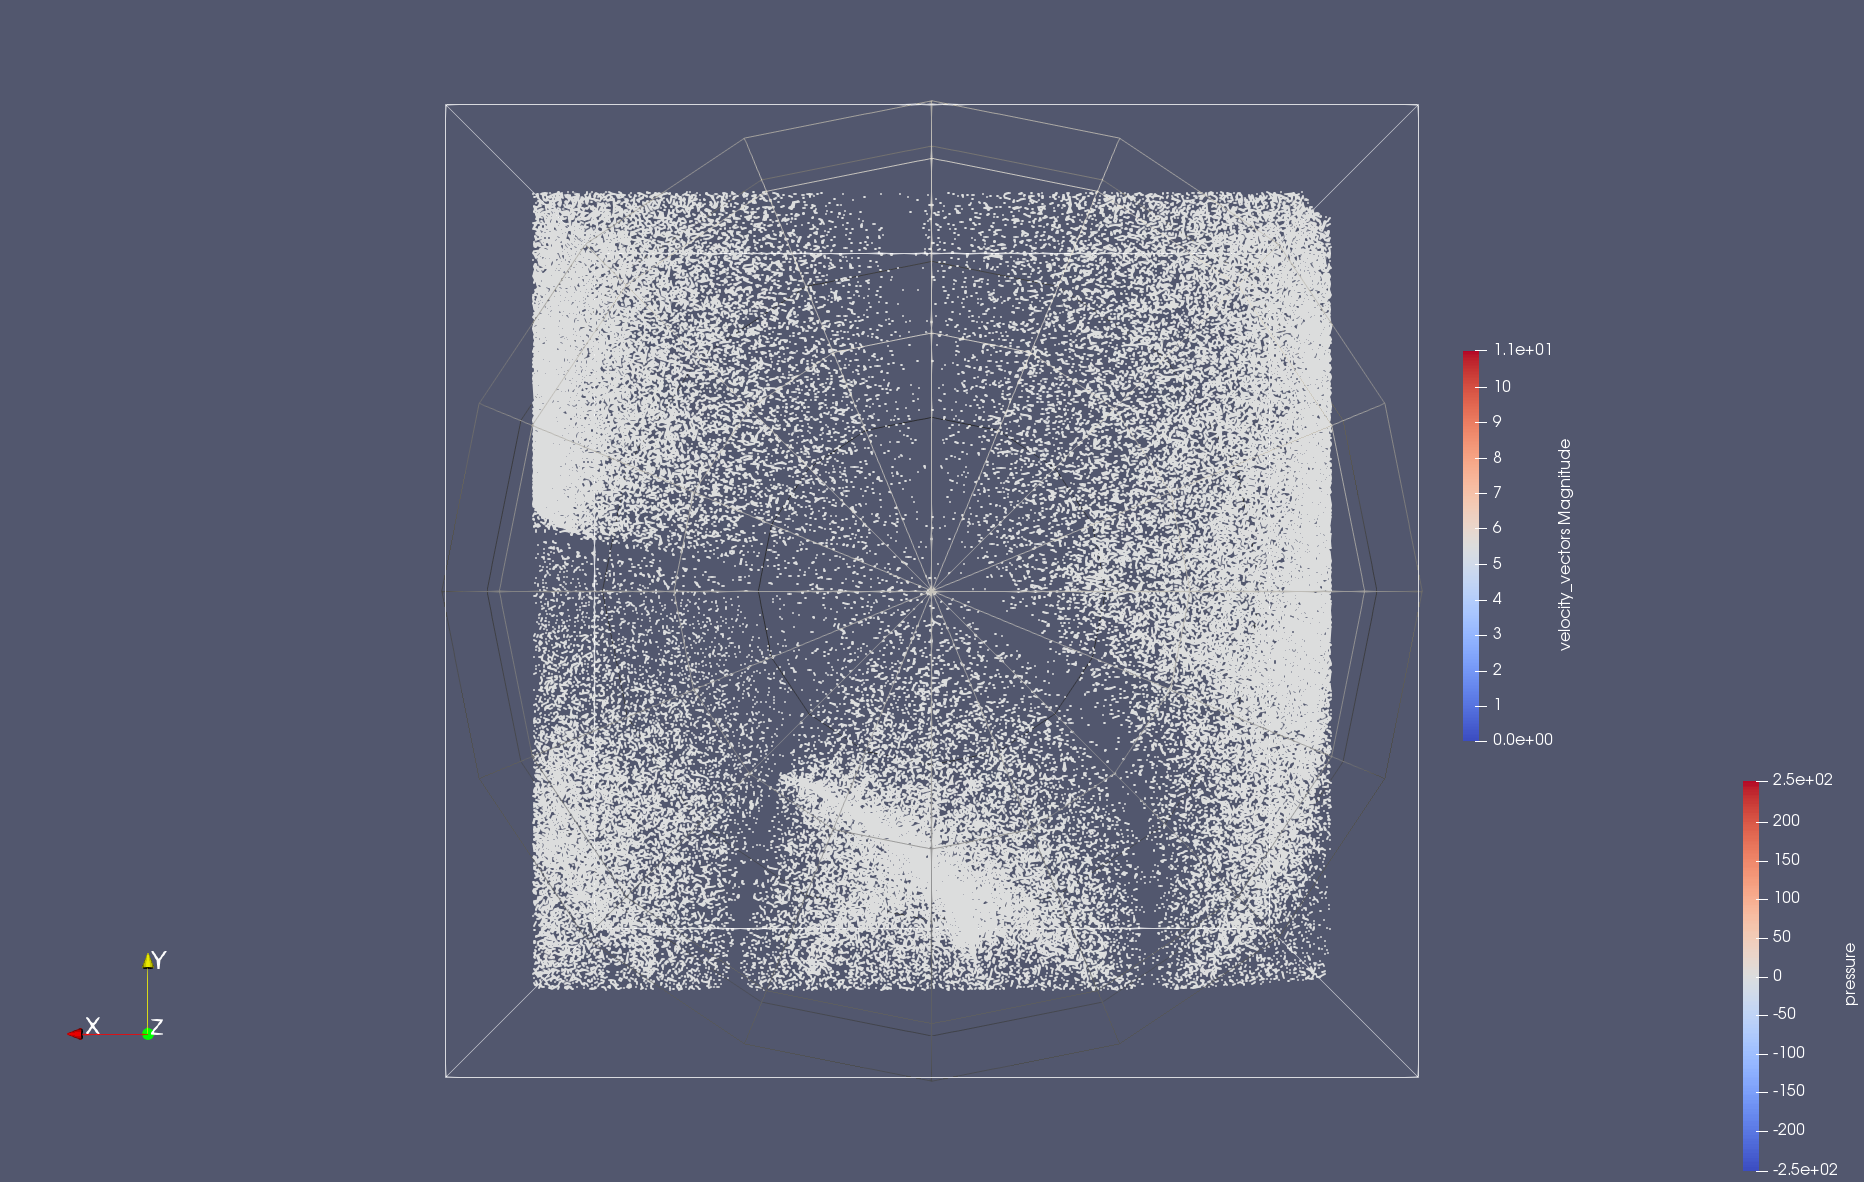
\includegraphics[height = 5cm, keepaspectratio]{graphes/Paraview/section_pioncarre_R_8_maillage_double.png}
        \caption{R = 8}
    \end{minipage}
\end{figure}
\begin{figure}[!h]
    \begin{minipage}[c]{.46\linewidth}
        \centering
        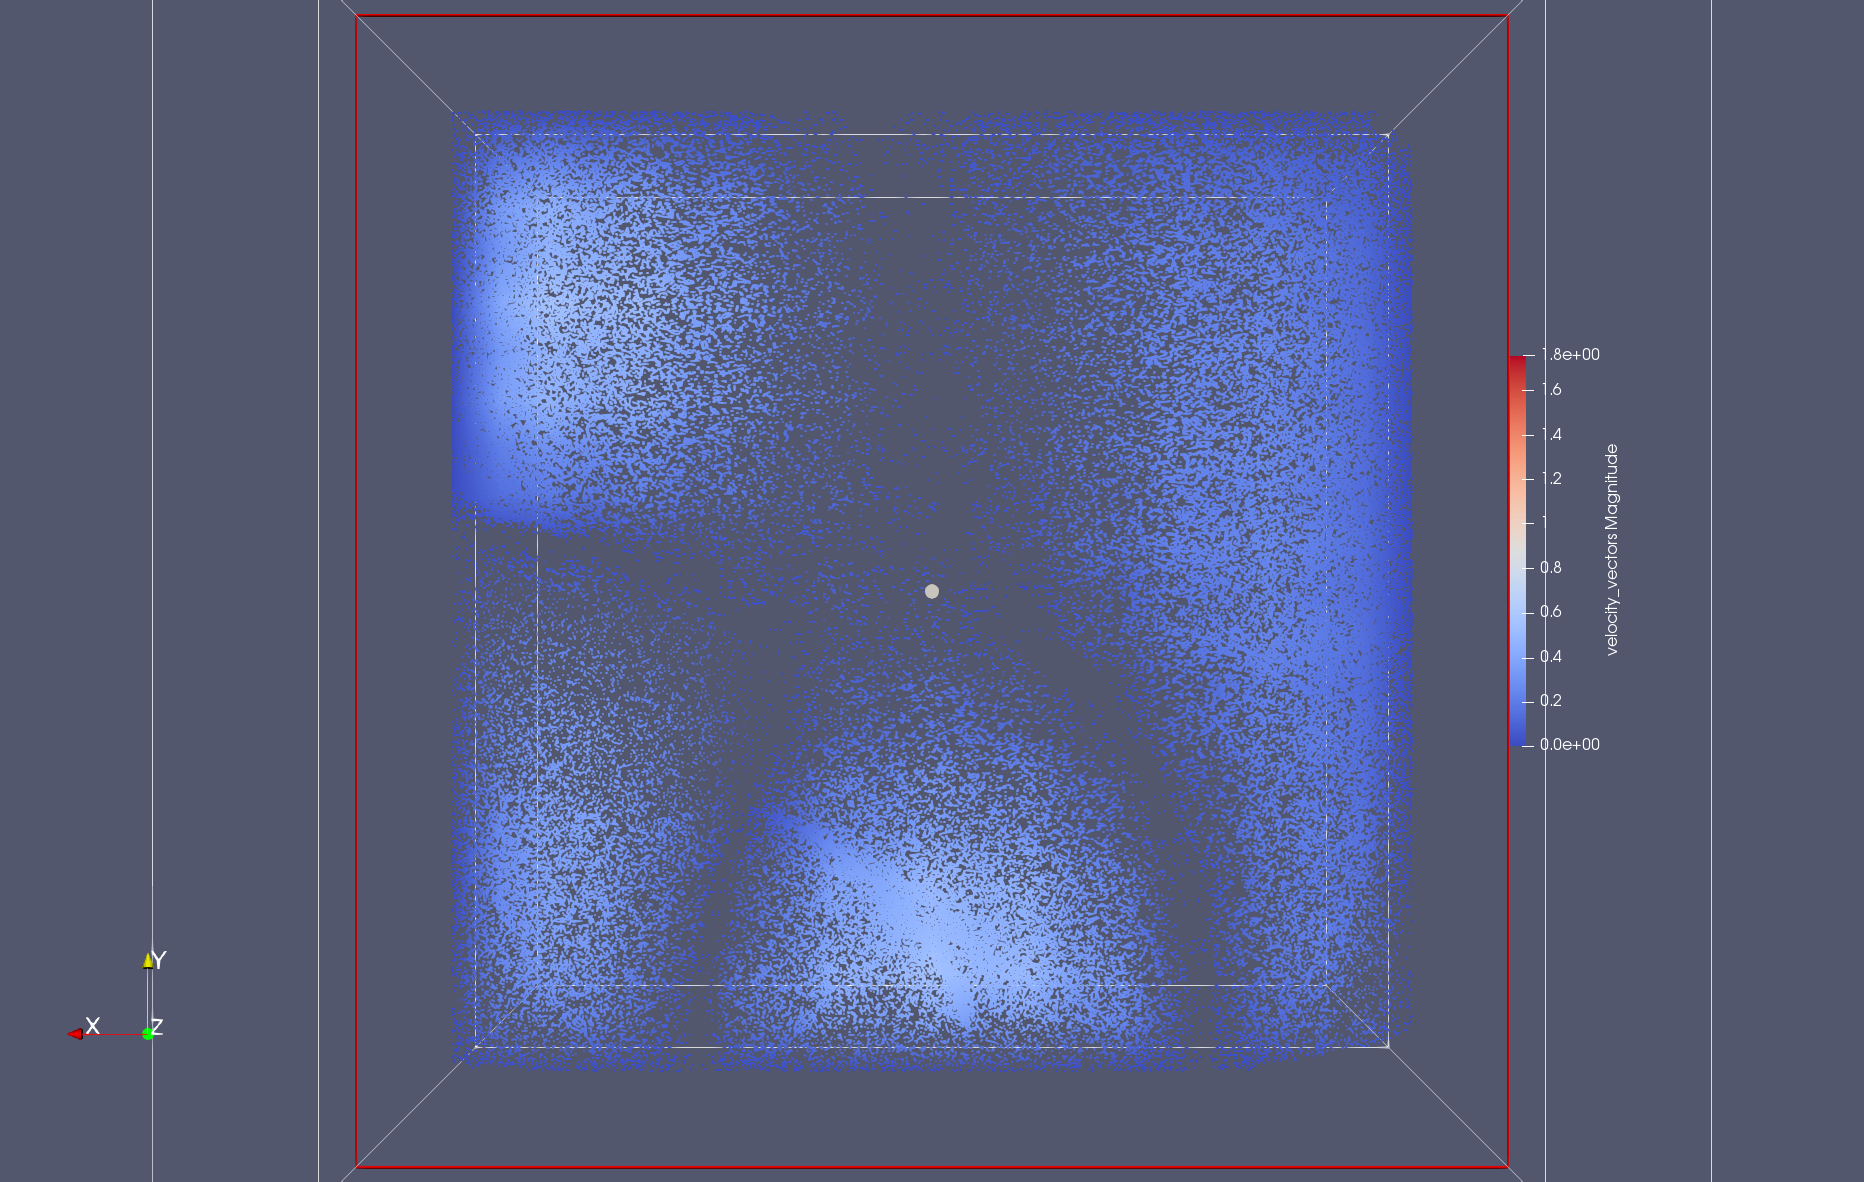
\includegraphics[height = 5cm, keepaspectratio]{graphes/Paraview/section_pioncarre_R_5.png}
        \caption{R = 5}
    \end{minipage}
    \hfill%
    \begin{minipage}[c]{.46\linewidth}
        \centering
        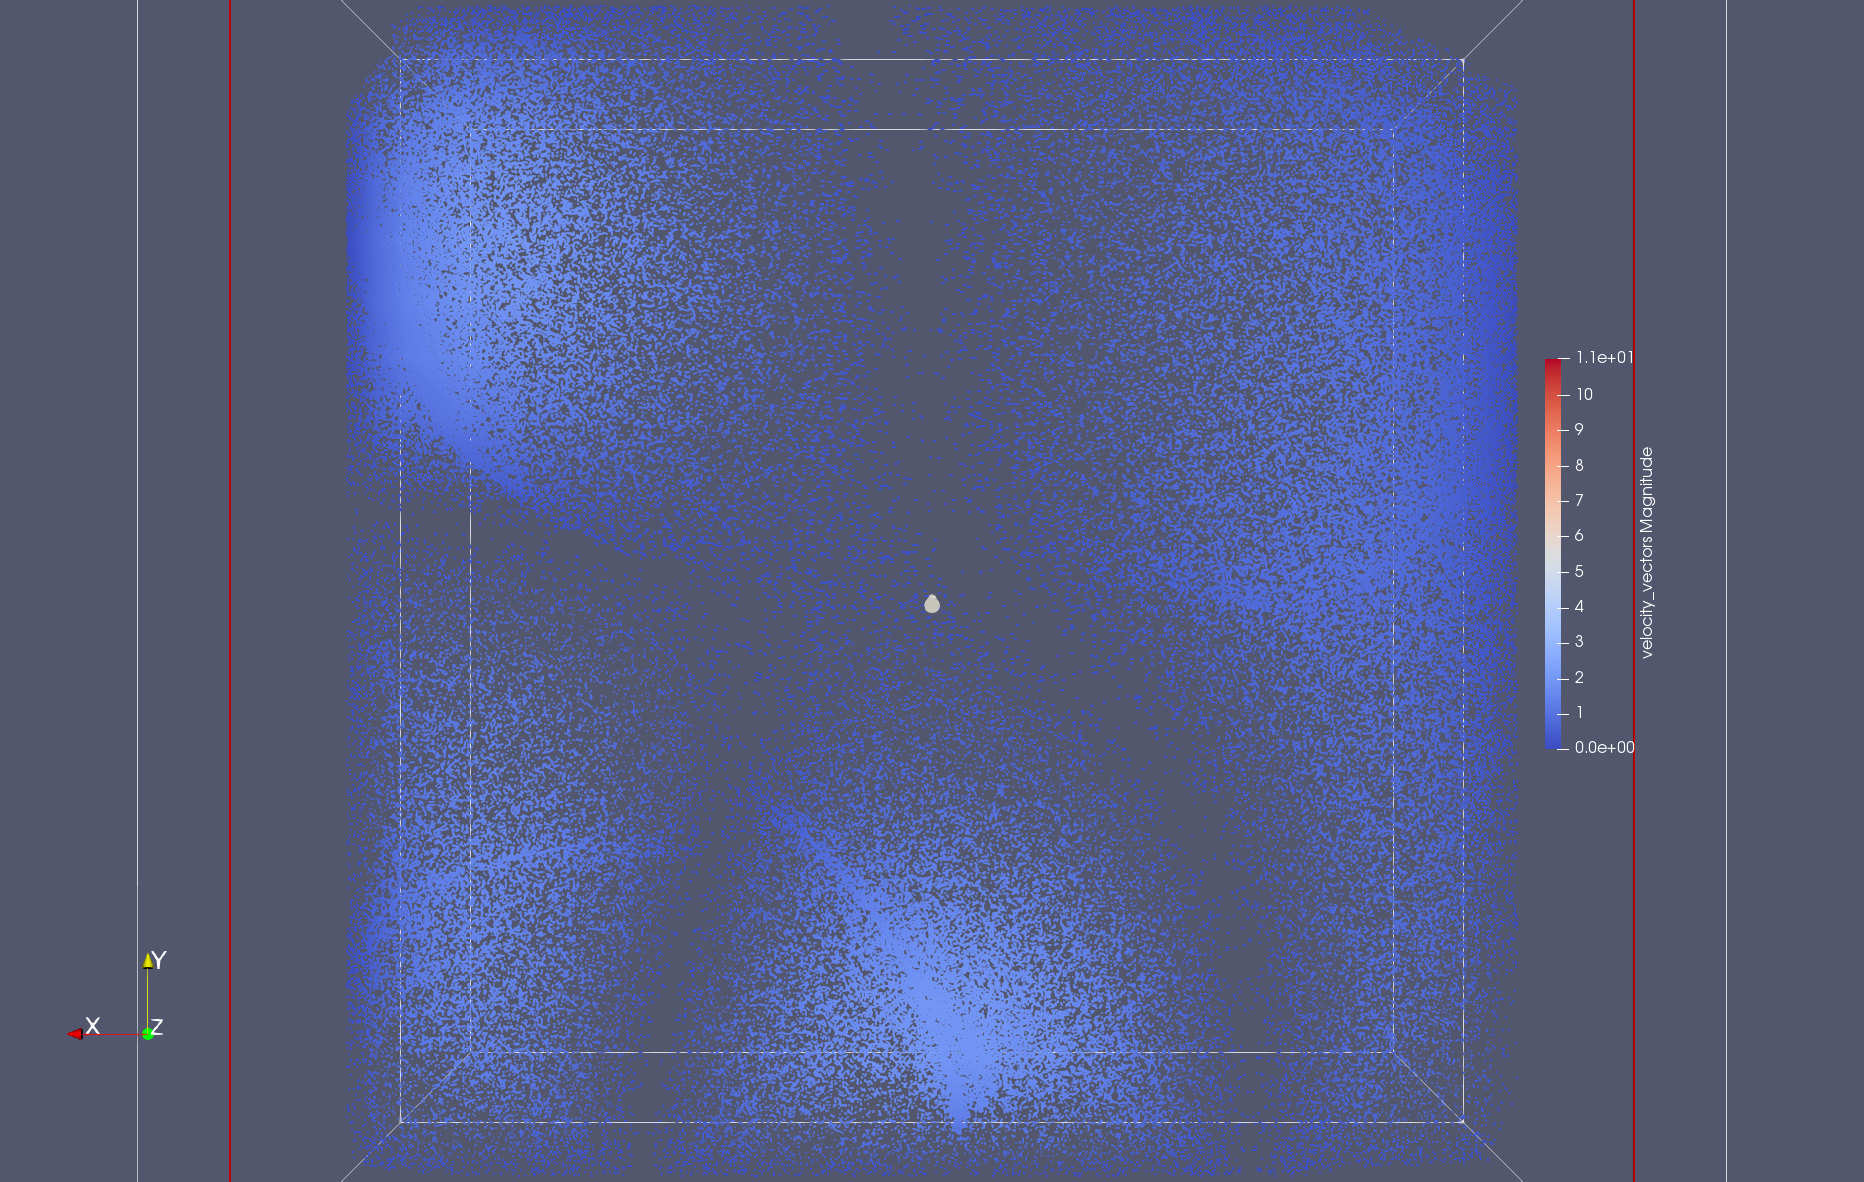
\includegraphics[height = 5cm, keepaspectratio]{graphes/Paraview/section_pioncarre_R_2_double.png}
        \caption{R = 2}
    \end{minipage}
\end{figure}
\begin{figure}[!h]
    \begin{minipage}[c]{.46\linewidth}
        \centering
        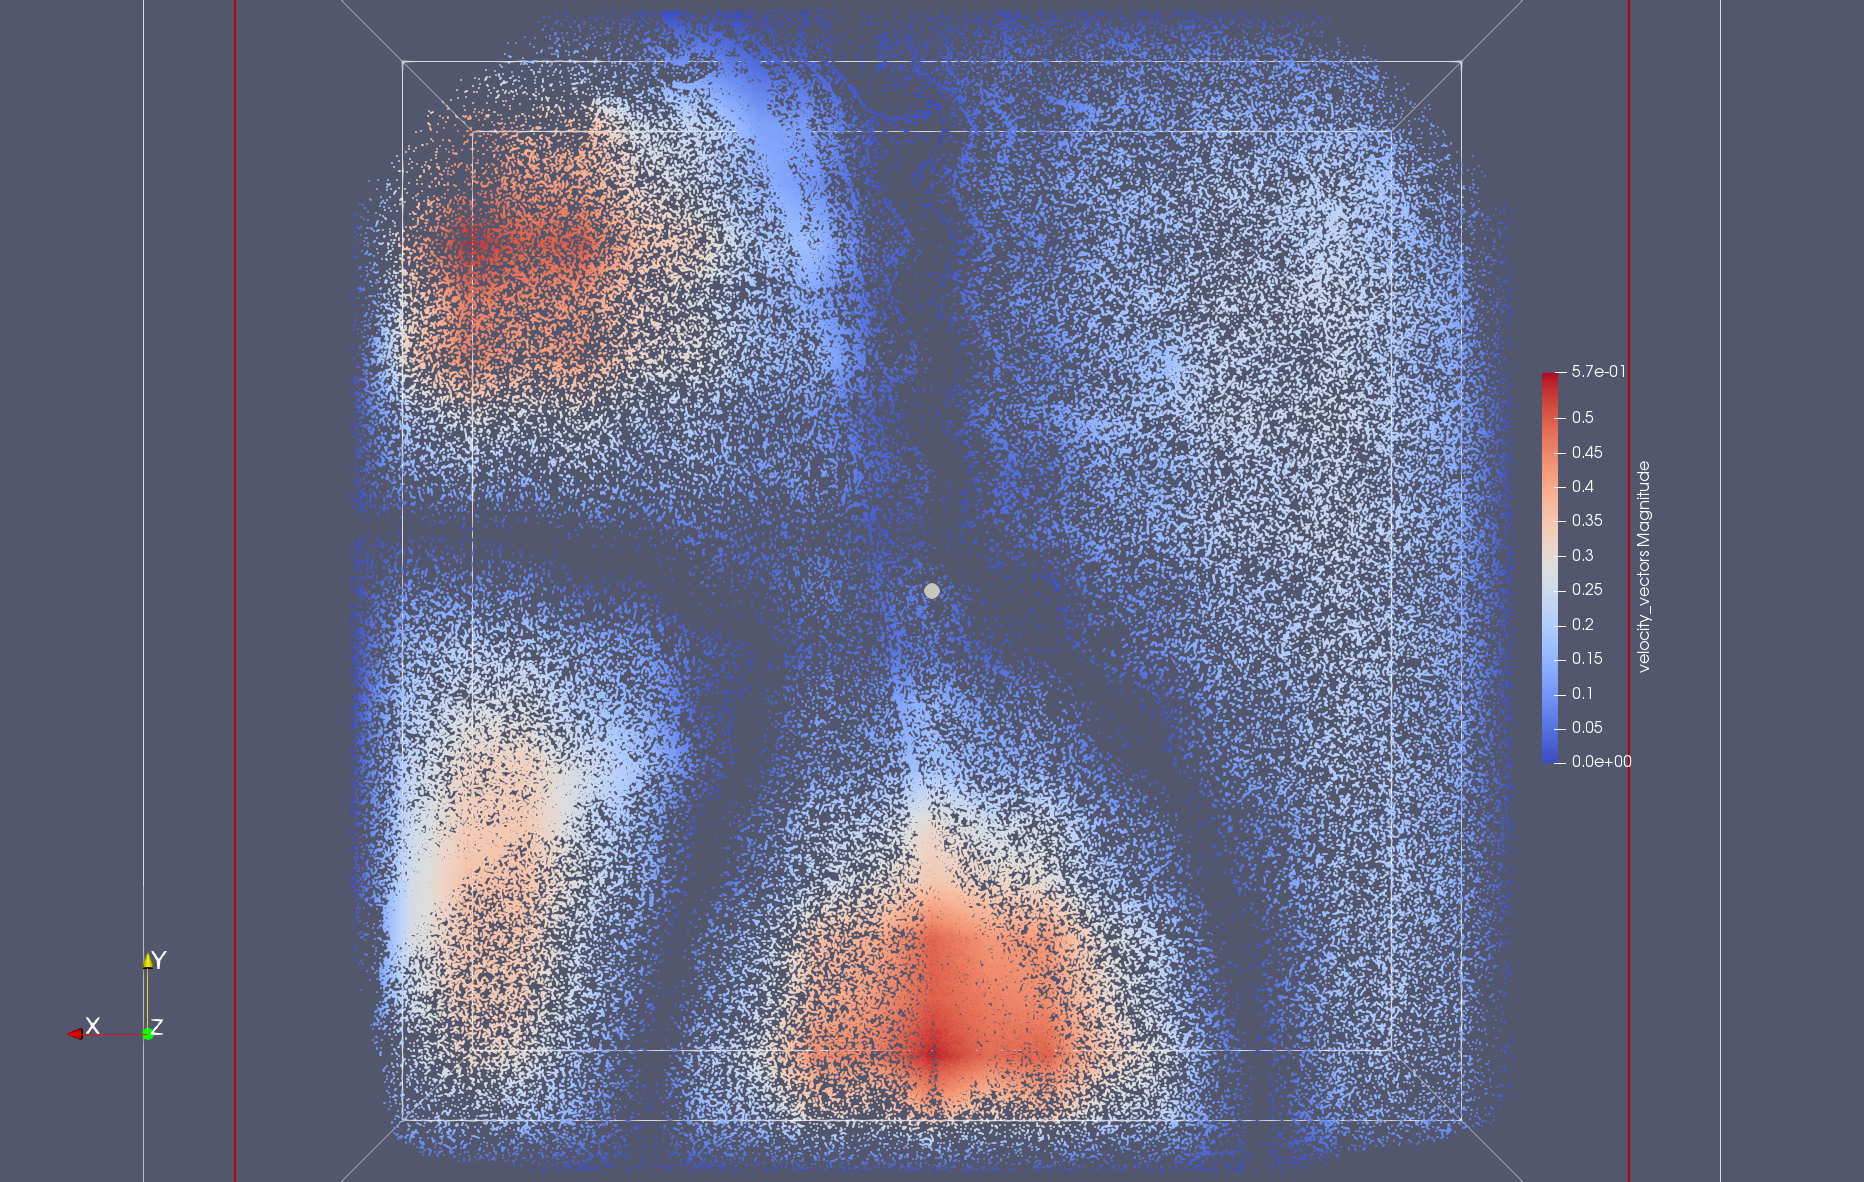
\includegraphics[height = 5cm, keepaspectratio]{graphes/Paraview/section_pioncarre_R_01.png}
        \caption{R = 0.1}
    \end{minipage}
    \hfill%
    \begin{minipage}[c]{.46\linewidth}
        \centering
        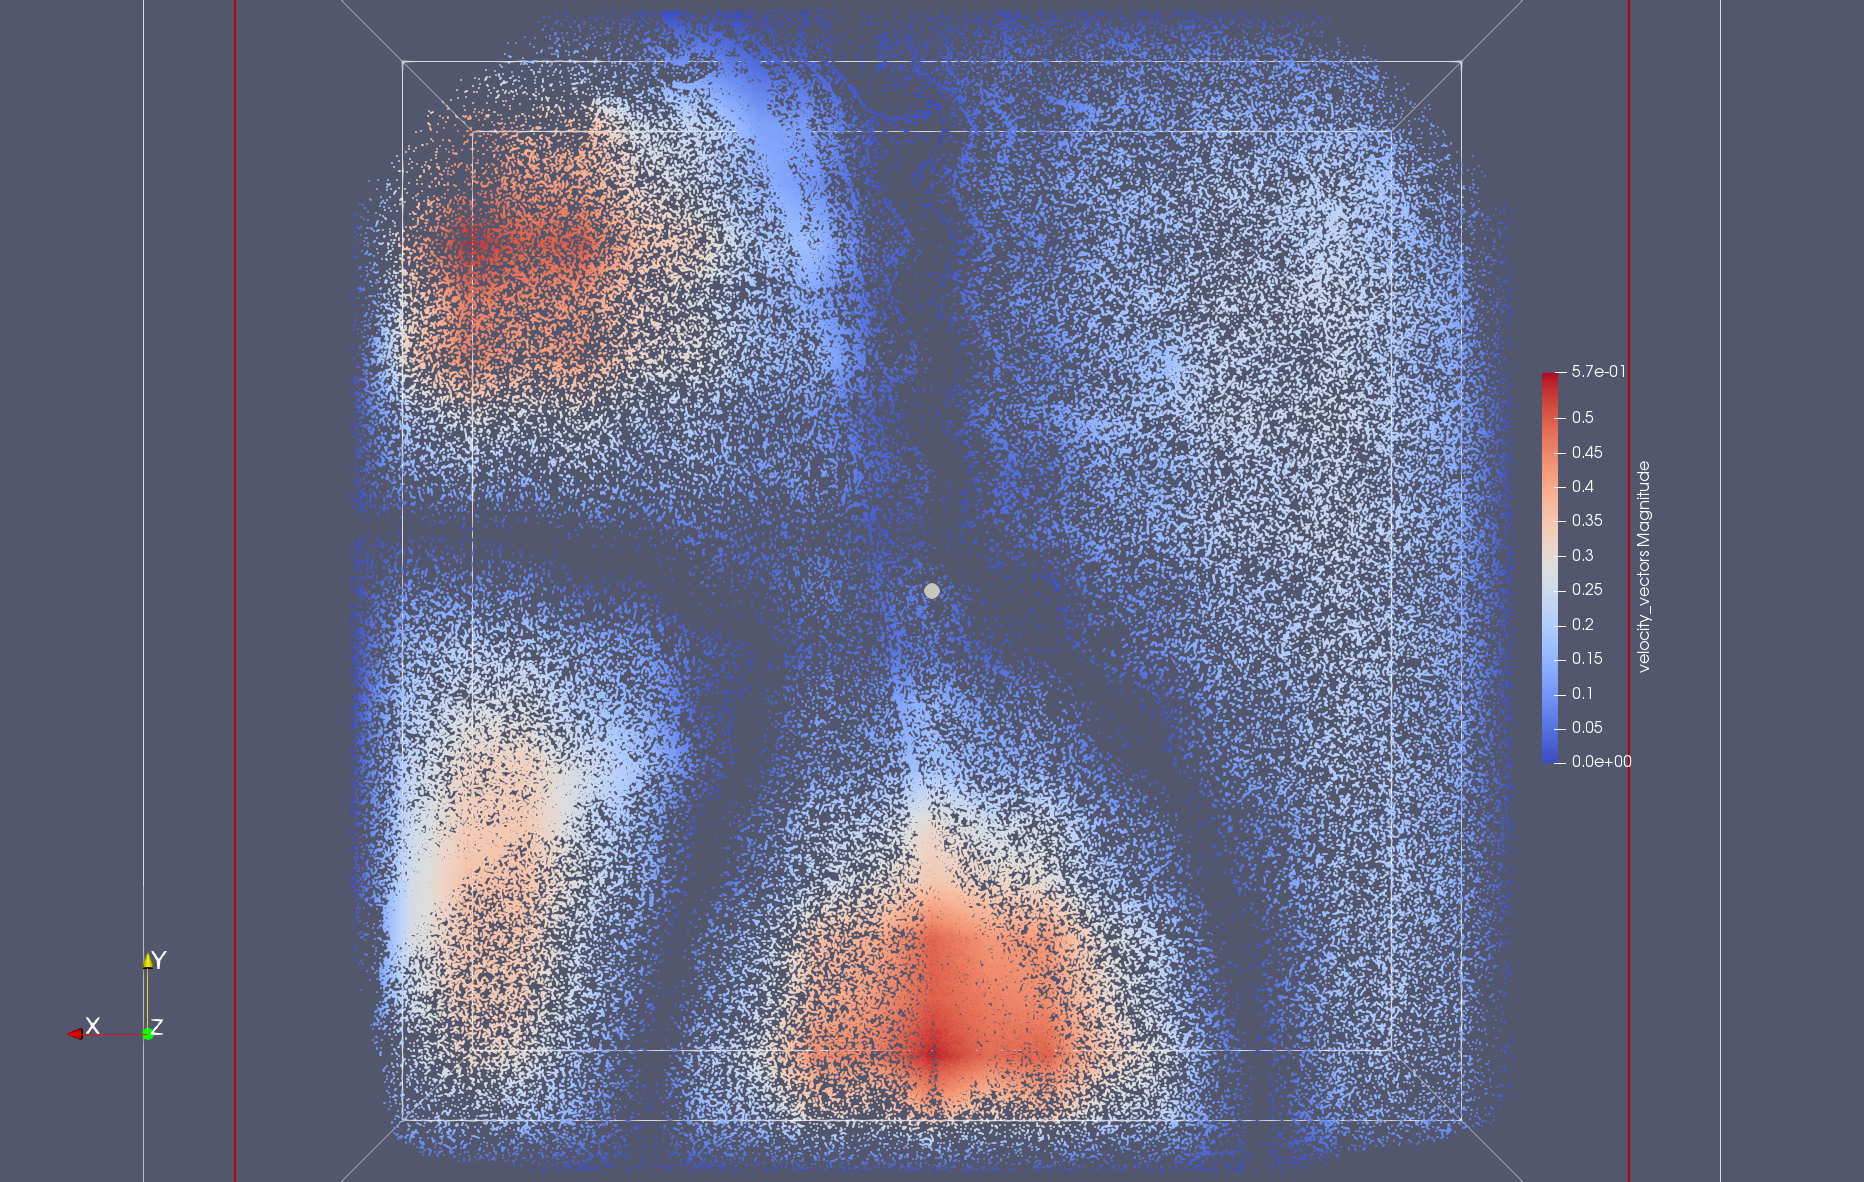
\includegraphics[height = 5cm, keepaspectratio]{graphes/Paraview/section_pioncarre_R_01.png}
        \caption{R = 0.5}
    \end{minipage}
\end{figure}
\begin{figure}[!h]
    \begin{minipage}[c]{.46\linewidth}
        \centering
        \includegraphics[height = 5cm, keepaspectratio]{graphes/Paraview/section_pioncarre_R_001_double.png}
        \caption{R = 0.01}
    \end{minipage}
    \hfill%
    \begin{minipage}[c]{.46\linewidth}
        \centering
        \includegraphics[height = 5cm, keepaspectratio]{graphes/Paraview/section_pioncarre_R_005_double.png}
        \caption{R = 0.05}
    \end{minipage}
\end{figure}
\begin{figure}[!h]
    \begin{minipage}[c]{.46\linewidth}
        \centering
        \includegraphics[height = 5cm, keepaspectratio]{graphes/Paraview/section_pioncarre_R_0005_double.png}
        \caption{R = 0.005}
    \end{minipage}
    \hfill%
\end{figure}

On voit en comparant aux sections de Poincaré réalisées l'année dernière que les zones sombres correspondants à des points dispersé, c'est à dire des zones chaotiques, ont tendance à être courbées alors qu'elles avaient tendance à être droites dans l'hypothèse du champ magnétique uniforme sur une partie de la cuve et nul ailleurs.
Nous n'observons pas cette "plage du chaos" correspondant à un élargissement de ces zones sombre en fonction de la valeur du coefficient R.
Malheureusement, malgrès notre tâtonnement sur la valeur de R nous ne sommes pas arrivé à cerner la plage de valeurs pour laquelle l'écoulement est chaotique, malgrés également que nous ayant divisé par deux le pas de maillage. Cela nécessite sans aucun doute des simulations plus poussés mais nous avons malheureusement tardé à avoir ces résultats ce qui ne nous à pas permis d'avoir le temps de lancer une série de simulations plus complètes déja que les simulations actuelles entre la résolution du système linéaire et l'interpolation sous Paraview peuvent prendre un temps non négligeable. Ce que nous aurions du notamment faire est de prendre un paramètre $Maximum$ $StreamLine$ $Length$ beaucoup plus important comme l'année dernière. De manière générales les simulations réalisé l'année dernière en terme de pas de pas de maillage, de nombre de point, et de $Maximum$ $StreamLine$ $Length$ sont beaucoups plus poussées que celle que nous avons réalisés. Nous avons tenté des simulations sous Paraview avec le même paramètrage que l'année dernière mais nous nous confrontons à un problème de stabilité du logiciel.
Nous réesayerons néanmoins d'ici la soutenance d'arriver à faire tourner une simulation plus fine qui pourrait être intéressante.\\
\newpage
%======================== Conclusion ================================================================
\newpage
\textbf{\Huge Conclusion:}
\normalsize
\\

L'objectif de ce projet a été, en partant de la thèse de Valérie Toussaint, de pousser l'étude des écoulement chaotiques avec un dispositif expérimental à 3 tourbillons. \\
\\
La valeur ajouté que nous devions apporter est une simulation se rapprochant plus du réel en ne supposant pas le champ magnétique uniforme sur une moitié de la cuve. Nous avons put voir des modifications intéressantes sur les  tourbillons en supprimant cette hypothèse.\\
Cependant en utilisant les sections de Poincarré de manière empirique nous n'avons pas identifié "la plage du chaos" qui permet en modulant selon un rapport R les forces des deux aimant d'arriver à un écoulement chaotique sur une portion majoritaire du fluide. \\
Un autre objectif de ce projet était la caractérisation mathématique de l'advection chaotique en calculant les exposant de Lyapunov et en étudiant l'évolution de la distance entre deux particule se trouvant à une distance $\delta x$ l'une de l'autre à l'instant initial. Le but de cette étude mathématique aurait été la recherche plus précise du rapport R optimal pour générer le choaos face à l'approche des section de Poincaré qui est empirique.
%==========================================================================================================================================================
%														Annexe
%==========================================================================================================================================================

\begin{appendix}

%================================ matrice de rigidité ====================================================================
\chapter{Calcul de la matrice de rigidité}
\label{annexe_1}

La matrice Jacobienne de la transformation est définie par
\[	
J =
\begin{pmatrix}
  \frac{\partial\varphi_{1}}{\partial \hat{x}_{1}} & \frac{\partial\varphi_{2}}{\partial \hat{x}_{2}}  & \frac{\partial\varphi_{3}}{\partial \hat{x}_{1}}\\ 
  \frac{\partial\varphi_{1}}{\partial \hat{x}_{2}} & \frac{\partial \varphi_{2}}{\partial \hat{x}_{2}} & \frac{\partial\varphi_{3}}{\partial \hat{x}_{2}} 
\end{pmatrix} 
\times
\begin{pmatrix}
   x_{1} &  y_{1} \\
   x_{2} &  y_{2} \\
   x_{3} &  y_{3}
\end{pmatrix}
\]
\[
\frac{\partial \hat{\varphi}}{\partial \hat{x}_{1}}(\hat{x}) = 
\frac{\partial}{\partial \hat{x}_{1}}(\varphi(F(\hat{x})) = 
\frac{\partial \varphi}{\partial x_{1}}(x) \frac{\partial F_{1}}{\partial \hat{x}_{1}}(\hat{x}) +
\frac{\partial \varphi}{\partial x_{2}}(x) \frac{\partial F_{2}}{\partial \hat{x}_{1}}(\hat{x})
\]

Donc
\[ \bigtriangledown_{\hat{x}} \hat{\varphi} = 
\begin{pmatrix}
   \frac{\partial F_{1}}{\partial \hat{x}_{1}} & \frac{\partial F_{2}}{\partial \hat{x}_{2}}\\
\end{pmatrix}
\times 
\begin{pmatrix}
   \frac{\partial \varphi}{\partial x_{1}}(x) \\
   \frac{\partial\varphi}{\partial x_{2}}(x)
\end{pmatrix} = 
J^{T} \times \bigtriangledown_{x} \varphi \]

Calculons $\bigtriangledown_{\hat{x}} \hat{\varphi}$ sur le triangle de référence $\hat{T}$ :
\[
\left\{
\begin{array}{ccc} 
	\begin{aligned}
		\hat{\varphi}_{1} &= -\hat{x}_{1}+1-\hat{x}_{2} \\  %\qquad 	
		\hat{\varphi}_{2} &= \hat{x}_{1}                \\  %\qquad 
		\hat{\varphi}_{3} &= \hat{x}_{2}
	\end{aligned}
\end{array}
\right.
\]
En effet $\hat{\varphi}_{1}$ vaut 1 sur le sommet 1 et 0 sur les autres sommets (Figure 3).
Ainsi
\[ \bigtriangledown_{\hat{x}} \hat{\varphi}_{1} = 
\begin{pmatrix}
   -1 \\
   -1
\end{pmatrix}
\qquad
\bigtriangledown_{\hat{x}} \hat{\varphi}_{2} = 
\begin{pmatrix}
   -1 \\
   -1
\end{pmatrix}
\qquad
\bigtriangledown_{\hat{x}} \hat{\varphi}_{1} = 
\begin{pmatrix}
   -1 \\
   -1
\end{pmatrix}
\]
et donc
\[
\bigtriangledown_{\hat{x}} \hat{\varphi}(\hat{x}) = 
\begin{pmatrix}
   -1 & 1 & 0 \\
   -1 & 0 & 1 
\end{pmatrix}
\]
\[	
J =
\begin{pmatrix}
   -1 & 1 & 0 \\
   -1 & 0 & 1 
\end{pmatrix}
\times
\begin{pmatrix}
   x_{1} &  y_{1} \\
   x_{2} &  y_{2} \\
   x_{3} &  y_{3}
\end{pmatrix} =
\begin{pmatrix}
   x_{2}-x_{1} &  y_{2}-y_{1} \\
   x_{3}-x_{1} &  y_{3}-y_{1}
\end{pmatrix}
\]
Finalement,
\[
\begin{vmatrix}
   J
\end{vmatrix}
= (x_{2}-x_{1})\times (y_{3}-y_{1})-(x_{3}-x_{1})\times(y_{2}-y_{1})= 2\times\text{Aire}(T)
\]
où $|J|$ est le déterminant de la matrice $J$
et ainsi
\[ \bigtriangledown_{x} \varphi =  (J^{-1})^{T} \times \bigtriangledown_{\hat{x}} \hat{\varphi} \]
avec
\[
J^{-1} =  \frac{1}{|J|}
\begin{pmatrix}
   J_{22} & -J_{12} \\
   -J_{21} & J_{11}
\end{pmatrix}
\]
d'où
\[
*\begin{aligned}
	(J^{-1})^{T} 
	&=  	
	\frac{1}{|J|}
	\begin{pmatrix}
   		J_{22} & -J_{21} \\
   		-J_{12} & J_{11}	
	\end{pmatrix} \\
	&=
	\frac{1}{2\times \text{aire}(T)}
	\begin{pmatrix}
   		J_{22} & -J_{21} \\
   		-J_{12} & J_{11}	
	\end{pmatrix} 
	\end{aligned}
\]

Et le calcul du terme $A_{ij}$ de la matrice de rigidité, on obtient ainsi avec le changement de variable vers le triangle de référence.
\[
\begin{aligned}
	\text{A}_{ij} 
	&=
	\sum_{T \in \text{Supp}(\varphi_{i})\times \text{Supp}(\varphi_{j})} 
	\iint_{(i,j) \in T}\bigtriangledown_{x}{\varphi_{i}} \bigtriangledown_{x}{\varphi_{j}} \\
	&=
	\sum_{T \in \text{Supp}(\varphi_{i})\times \text{Supp}(\varphi_{j})}
	\iint_{(i,j) \in T} (J^{-1})^{T}|J|(J^{-1})^{T}|J|
	\times
	\bigtriangledown_{\hat{x}} \hat{\varphi_{i}}
	\times
	\bigtriangledown_{\hat{x}} \hat{\varphi_{j}} \\
	&=
	\sum_{T \in \text{Supp}(\varphi_{i})\times \text{Supp}(\varphi_{j})}	
	\frac{\text{aire}(T)^{2}}{4}
	\begin{pmatrix}
   		y_{3}-y_{1} &  	x_{1}-x_{3}\\
   		y_{1}-y_{2} &  x_{2}-x_{1}
	\end{pmatrix}
	^{2}
	\bigtriangledown_{\hat{x}} \hat{\varphi_{i}}
	\bigtriangledown_{\hat{x}} \hat{\varphi_{j}}
\end{aligned}
\]

%================================= CODE MATLAB ===========================================================================

\chapter{Codes Matlab}
\label{annexe_2}

\subsection{Modélisation du champ magnétique}
\small

\begin{verbatim}
%==========================================================================
%         Calcul (exact) des matrices P1 de masse et de rigidite
%==========================================================================
function [A, M, nn, ibint, ic2] = matrixP1final(vz,tz,fnum,node1,edge1,node2,edge2)
%-------------------------- initialisation ----------------------------------
nt = size(tz,1);                     %nombre de triangle
nn = size(vz,1);                     %nombre de noeuds
v1 = [vz findedge(vz,node1,edge1,0.001)];%calcul label des noeuds,
										% si il sont sur un bord
%matrices elementaire des gradients dans le triangle de reference
grad_elem = [-1 1 0;
             -1 0 1];
   ind_ligne = 1;              %initialisation premiere ligne
%-------------------------- boucle ---------------------------------------   
for k = 1:nt				% on boucle sur les triangles du maillage
        Tk = tz(k,1:3);    %on recupere les noeuds definisant le triangle k  [n1 n2 n3]
%--------------------------------------------------------------------------   
%                        calcul du terme source M
%--------------------------------------------------------------------------
    if fnum(k) == 1      %on teste si le triangle est sur le maillage de l'aimant                                    
		l = v1(Tk,3);    %l regroupe les valeurs des labels
	    vN1 = v1(Tk,1:3); %coordonees des noeuds du triangle
	    if (size(l(ismember(l,0))) == [1 1]) | (size(l(ismember(l,0))) == [0 1])
    		compter = sum(l == l');
        	z = vN1(:,3) ~= l(compter == 1);
			if size(z(ismember(z,0))) == [1 1]       %on elimine le cas d'un 
			%triangle bizarre a cheval sur 2 bords
        		Nb = vN1(z,1:2);  %on recupere les coordonnees des noeuds du 
        		%triangles qui sont sur le bord 
            	NNb = Tk(z);    %on recupere les numeros des triangles sur le bord
           		Ni = vN1(vN1(:,3)==l(compter==1),1:2);  %noeuds interieurs
           		%on calcule la norme de l'arete
          	  	norme_e = sqrt((Nb(1,2) - Nb(2,2))^2 + (Nb(1,1) - Nb(2,1))^2);  
           		n_normal = [Nb(2,2)-Nb(1,2); Nb(1,1)-Nb(2,1)];  %vecteur normal a l'arete
            	n_test = [Ni(1,1)-Nb(1,1); Ni(1,2)-Nb(1,2)];
   	        	if n_normal'*n_test < 0       %on teste si le vecteur normal 
   	        	%que l'on a calcule est dans le bon sens
            	n_normal = -n_normal;         %dans ce cas on le prend dans 
            	%l'autre sens pour qu'il soit sortant
         		end
     			M_inter =  (norme_e / 2).*[0 ; 1]'*n_normal;%[0;1] correspond au vecteur ey
    			M(NNb,:) =  M(NNb,:) + M_inter;  %on place la valeur corespondant
    			% a l'arete dans la matrice du terme source 
        	end                                                              
        end
    end
%--------------------------------------------------------------------------
%                             matrice de rigidite
%--------------------------------------------------------------------------                     

	pk = vz(Tk,1:2);     %3*2 coordonnees des noeuds triangle k 
    indice=Tk'*ones(1,3);%3*3 chaque colonne [n1 n1 n1 ;n2 n2 n2;n3 n3 n3] 
    %noeuds du triangle i
    ligne(ind_ligne:ind_ligne+8) = indice(:); %on stocke sous la forme de colonne
    indice=indice';                                 
   	colonne(ind_ligne:ind_ligne+8) = indice(:); %[n1;n1;n1;n2;n2;n2;n3;n3;n3]
       
    %implementation de A
    A_inter matrice elementaire 3*3 des gradients dans le triangle k
    terme_jacobien = (airek^2)/4 .* ([pk(3,2)-pk(2,1) pk(1,1)-pk(3,1) ;..
    pk(2,1)-pk(2,2) pk(2,1)-pk(1,1)]^2);
    A_inter = zeros(3,3);
    A_inter(1,1) = (terme_jacobien*grad_elem(:,1))'*grad_elem(:,1);
    A_inter(2,2) = (terme_jacobien*grad_elem(:,2))'*grad_elem(:,2);
    A_inter(3,3) = (terme_jacobien*grad_elem(:,3))'*grad_elem(:,3);
    A_inter(1,2) = (terme_jacobien*grad_elem(:,1))'*grad_elem(:,2);
    A_inter(1,3) = (terme_jacobien*grad_elem(:,1))'*grad_elem(:,3);
    A_inter(2,3) = (terme_jacobien*grad_elem(:,2))'*grad_elem(:,3);
    A_inter(2,1) = A_inter(1,2); 
    A_inter(3,1) = A_inter(1,3); 
    A_inter(3,2) = A_inter(2,3);        
    A_inter = A_inter(:);
    A_val(ind_ligne:ind_ligne + 8) = A_inter;
           
    ind_ligne = ind_ligne + 9;      %iteration
end
%on place les valeurs calcules avec les valeurs des noeuds
        A = sparse(ligne,colonne,A_val);   %on place les valeurs calcules 
        %avec les valeurs des noeuds
%----------- On ne retient que les noeuds interieurs ----------------------------
ic2 = (1:nn)';  
ibint = v2(:,3)~= 0;  %noeuds du bord de la face 2_exterieure
ic2(ibint) = [];      %liste des noeuds interieur au maillage total
A = A(ic2,ic2);   %on ne garde que les noeuds interieurs
M = ones(nn,1); 
end
\end{verbatim}

\begin{verbatim}
%=========================================================================
%                       Calcul du gradient du potentiel U
%=========================================================================
function [B] = gradient(u,v,t);
%           retourne B matrice n*2 [B_x B_y]
%           u matrice colonne des potentiels u
%           v matrice colonne des coordonées des noeuds
%           t table de connectivité
%---------------- initialisation -------------------------------------------------
nt = size(t,1);   %nombre de triangle
nn = size(v,1);   %nombre de noeuds
grad_elem_ref = [-1 1 0;   %gradients sur le triangle de référence
                 -1 0 1];
ind_ligne = 1;  %initialisation premiere ligne
M_elem = [ 2 1 1;        %matrice de masse elementaire
	       1 2 1;
	       1 1 2]/12;
M_elem = M_elem(:);
M_val = zeros(nt*9,1);
%-------------------- boucle sur les triangles ---------------------------------
for k = 1:nt
	Tk = t(k,1:3);  %on recupere les noeuds definisant le triangle k  [n1 n2 n3]
    vk = v(Tk,1:2); %coordonnées des noeuds du triangle k   
    airek = t(k,5); %aire du triangle k
%on recupere les indices des neuds pour ensuite placer les 9
%contributions du triangle k dans la matrice C
    indice=Tk'*ones(1,3); %3*3 chaque colonne [n1 n1 n1 ;n2 n2 n2;n3 n3 n3] 
    ligne(ind_ligne:ind_ligne+8)=indice(:); %on stocke sous la forme de colonne
    indice=indice';                                 
    colonne(ind_ligne:ind_ligne+8)=indice(:);  %[n1;n1;n1;n2;n2;n2;n3;n3;n3]
%---------------------- Calcul matrice C --------------------------------
%Jacobien
	Jk = [vk(3,2)-vk(1,2) vk(1,1)-vk(3,1); vk(1,2)-vk(2,2) vk(2,1)-vk(1,1)];
	grad_elem = Jk' * grad_elem_ref;  %Calcule le gradient dans triangle a 
	%partir triangle de reference
	C_elem_x1 = (1/6) * [ grad_elem(1,1)*ones(1,3);
                      grad_elem(1,2)*ones(1,3);
                      grad_elem(1,3)*ones(1,3)];
	C_elem_x1 = C_elem_x1(:);
	C_val_x1(ind_ligne:ind_ligne + 8) = C_elem_x1;
	C_elem_x2 = (1/6) * [ grad_elem(2,1)*ones(1,3);
                      grad_elem(2,2)*ones(1,3);
                      grad_elem(2,3)*ones(1,3)];
	C_elem_x2 = C_elem_x2(:);
	C_val_x2(ind_ligne:ind_ligne + 8) = C_elem_x2;
%----------------------- Calcul matrice M -----------------------------------------------
	M_val(ind_ligne:ind_ligne+8) = airek*M_elem;
	ind_ligne = ind_ligne + 9;      %itération
end
C_x1 = sparse(ligne,colonne,C_val_x1);     %on place les valeurs avec les nums des noeuds
C_x2 = sparse(ligne,colonne,C_val_x2);
M = sparse(ligne,colonne,M_val);
%------------------------  Resolution du systeme lineaire----------------------------------
B_x1 = M\(C_x1'*u);
B_x2 = M\(C_x2'*u);
B = [B_x1 B_x2];
end
\end{verbatim}

\begin{verbatim}
%===========================================================================
%			Résolution champ magnétique avec éléments finis P1
%===========================================================================
%------------------  elaboration du maillage ---------------------------------------------------------
a = 1; %taille de l'aimant carre de taille a
%taille de la cuve
L = 5; %longueur
H = 5; %hauteur
node1 = [-a,-a; a,-a; a,a; -a, a];    %liste des noeuds intérieurs
node2 = [-L,-H; L,-H; L,H; -L, H];    %liste des noeuds extérieurs
edge1 = [(1:size(node1,1))',[(2:size(node1,1))'; 1]];  %liste des arètes intérieures
edge2 = [1,2; 2,3; 3,4; 4,1];                          %liste des arètes extérieures
edge = [edge1; edge2+size(node1,1)];   %liste de toutes les arètes mises dans l'ordre
node = [node1; node2];                 %liste de tous les noeuds mises dans l'ordre
pas_h=0.2;                             %pas maximal du maillage
hdata = [];
hdata.hmax  = pas_h;
face{1} = 1:size(edge1,1);             %face de maillage interieure
face{2} = 1:size(edge,1);              %face de maillage exterieure
[v,t,fnum] = meshfaces(node,edge,face,hdata); %construction du maillage
;
%------------------ calcul matrices ---------------------------------------
[A, M, nn, ibint, ic2] = matrixP1final(v,t,fnum,node1,edge1,node2,edge2);
%------------------   résolution du systeme lineaire ---------------------------------------
A = A(ic2,ic2); %on ne resout que sur les noeuds interieurs
sol = A\M;
u = zeros(nn,1);
u(ic2) = sol;
u(ibint) = 0;  
B = gradient(u,v,t);
B_X = B(:,1);
B_Y = B(:,2);
%on recupere les coordonnées de chaque point du maillage
X = v(:,1);
Y = v(:,2);
end
\end{verbatim}


\subsection{Résolution des Equations de Navier Stokes}
\begin{verbatim}
%=========================================================================% 
%  Résolution finale avec superposition des deux tourbillons
%=========================================================================%
%--------------- initialisation -------------------------------------------
% rapport R entre les forces magnetique
R = 0.005;

%------- resolution dans la configuration aimant centre -------------------
[X2,Y2,Z2,Uxgd_centre,Uygd_centre,Uzgd_centre,Pgd_centre] = stokes_3D(true,R);


%----------- resolution dans la configuration aimant de cote --------------
[X2,Y2,Z2,Uxgd_cote,Uygd_cote,Uzgd_cote,Pgd_cote] = stokes_3D(false,R);

%----- transposition du champ de vitesse et somme ------------------------
[Uxgd_cote_transp,Uygd_cote_transp,Uzgd_cote_transp] = transposition_champ(Uxgd_cote,Uygd_cote,Uzgd_cote);
% prise en compte du rapport R
R_i = norm(Uxgd_centre(:)) / norm(Uxgd_cote_transp(:));
Uxgd_cote_transp = (R / R_i) .* Uxgd_cote_transp;
Uxgd_total = Uxgd_centre + Uxgd_cote_transp;
Uygd_total = Uygd_centre + Uygd_cote_transp;
Uzgd_total = Uzgd_centre + Uzgd_cote_transp;
\end{verbatim}
\begin{verbatim}
%=========================================================================%
% 	Résolution Equations de Stokes 3D dans le cube [0,Lx]x[0,Ly]x[0,Lz]
% 						Elements Finis Q2/Q1
%=========================================================================%
function [X2,Y2,Z2,Uxgd,Uygd,Uzgd,Pgd] = Stokes3D(aimant_centre,R)
% si aimant _centre = true l'aimant est centre, sinon non
%-------------- initialisation --------------------------------------------
global Lx Ly Lz %dimensions cuve
Lx=1;  % largeur
Ly=1;  % profondeur
Lz=1;  % hauteur
nu=1; % viscosité
% Nombres de points dans les directions x, y et z
Nx=21;
Ny=21;
Nz=21;
%----------- generation mailleur 3D ---------------------------------------
[v,t,nv1,nv2,nbquad,X,Y,Z] = mesh_3D(Lx,Ly,Lz,Nx,Ny,Nz);
% Recherche des points du bord pour le traitement des conditions aux 
% limites de Dirichlet
ind_bd=find(v(:,1)==0|v(:,1)==Lx|v(:,2)==0|v(:,2)==Ly|v(:,3)==0|v(:,3)==Lz);
ind_bd=unique(ind_bd);
%--------------------------------------------------------------------------
% Construction des matrices de Stokes 
%   A = [ a  b
%         b' 0]
%   Masse : matrice de masse
%--------------------------------------------------------------------------
[DxDx,DyDy,DzDz,DxDy,DxDz,DyDz,DxW,DyW,DzW,Masse]=matrix_3D(v,t);
A=[nu*(2*DxDx+DyDy+DzDz),              nu*DxDy',              nu*DxDz',             -DxW;
                  nu*DxDy, nu*(DxDx+2*DyDy+DzDz),              nu*DyDz',             -DyW;
                  nu*DxDz,               nu*DyDz, nu*(DxDx+DyDy+2*DzDz),             -DzW;
                    -DxW',                 -DyW',                 -DzW', sparse(nv1,nv1)];
% Construction du second membre
[fx, fy, fz, fxgd, fygd,fzgd,fxy] = f2Dto3D_2(v,t,nv1,nv2,nbquad,X,Y,Z,Nx,Ny,Nz,aimant_centre); 
%   fx, fy, fz sont les forces dans des vecteurs colonnes 1*size(v,1)
%   fxgd, fygd, fzgd sont les forces dans des matrices Nx*Ny*Ny pour
%   affichage
F=[fx; fy; fz; sparse(nv1,1)];
% Traitement de la pression a moyenne nulle par multiplicateur de Lagrange.
[A,F,nv1] = tmtpression(Nx,Ny,Nz,nv1,nv2,t,A,F);
% Traitement des CL
ibT=[ind_bd;ind_bd+nv2;ind_bd+2*nv2];
icT=(1:3*nv2+nv1);
icT(ibT)=[];
F(ibT)=[];
A = A(icT,icT);
%-------------------- Resolution du systeme lineaire Ax=F -----------------
[sol,residu,iter]=linsolver(A,F,nv1,nv2-length(ind_bd));
UP=zeros(3*nv2+nv1-1,1);
UP(icT)=sol;
% Vitesse
Ux=UP(1:nv2); Uy=UP(nv2+1:2*nv2); Uz=UP(2*nv2+1:3*nv2);
% Pression
Pr=UP((3*nv2+1):end);
% Interpolation de la pression sur le maillage Q2
nt1= (Nx-1)*(Ny-1)*(Nz-1); % nb de cubes Q1
Pr2 = build_Q2Pressure(t(1:nt1,:),Pr,nv2);

% Construction du maillage Q1-isoQ2
tQ1isoQ2 = meshQ1isoQ2(t); 
[X2,Y2,Z2,Uxgd,Uygd,Uzgd,Pgd] = gridformat(Lx,Ly,Lz,Nx,Ny,Nz,v,Ux,Uy,Uz,Pr2);
end
\end{verbatim}

\begin{verbatim}
%==========================================================================
%     		a partir d'un maillage donne f2Dto3D82 renvoit 
%   			le terme source f de l'equation de navier-stokes
%==========================================================================
function [fx, fy, fz, fxgd, fygd,fzgd,fxy] = f2Dto3D_2(v,t,nv1,nv2,nbquad,X,Y,Z,Nx,Ny,Nz,aimant_centre)
%   fx, fy, fz sont les forces dans des vecteurs colonnes 1*size(v,1)
%   fxgd, fygd, fzgd sont les forces dans des matrices Nx*Ny*Ny pour
%   affichage
%--------- extraction d'une couche 2d et triangulation --------------------
lz = 0;                             % niveau z=0
indz = find(v(:,3) == lz);
xz = v(indz,1); yz = v(indz,2); vz = [xz, yz];
tz = delaunay(xz,yz);              % triangulation de Delaunay des points du plan 

figure();
triplot(tz,xz,yz);   % affichage
title('couche 2D extraite du maillage 3D de la cuve')
%on voit que les point dans v ne sont pas dans l'ordre avec triplot         
%-------------------- coordonnées des differents maillage ------------------
node_ensemble = [0,0 ; 10 0; 10 10; 0 10]; %  maillage total
node_select = [4.5 4.5;5.5 4.5; 5.5 5.5; 4.5 5.5]; %  mailage cuve 
%---------- configuration aimant ------------------------------------------
if aimant_centre == true
    node_aimant = [4.75 3.5; 5.25 3.5; 5.25 4.5; 4.75 4.5]; 
end
if aimant_centre == false
    node_aimant = [5.1 3.5;5.6 3.5;5.6 4.5;5.1 4.5];       
end
edge_aimant = [(1:size(node_aimant,1))',[(2:size(node_aimant,1))'; 1]];       
edge_ensemble = [1,2; 2,3; 3,4; 4,1];                               
edge_total = [edge_aimant; edge_ensemble+size(node_aimant,1)];       
node_total = [node_aimant; node_ensemble];                      
%-------- generation maillage total de resolution du probleme 2D ------------
L_total = 10;
H_total = 10;
x_2D = linspace(0,L_total,2*10*(Nx-1) + 1)';
y_2D = linspace(0,H_total,2*10*(Ny-1) + 1 )';
[X_total_2D,Y_total_2D] = meshgrid(x_2D,y_2D);
v_total_2D_x = X_total_2D';
v_total_2D_x = v_total_2D_x(:);
v_total_2D_y = Y_total_2D';
v_total_2D_y = v_total_2D_y(:);
v_total_2D = [v_total_2D_x(:) v_total_2D_y(:)];
t_total_2D = delaunay(v_total_2D(:,1),v_total_2D(:,2)); %generation maillage triangulaire total
%---------- calcul du champ magnétique sur la couche z=0 ----------------- 
[B_X,B_Y] = champ_magnetique_fct_Tancrede_1(v_total_2D,t_total_2D,...
node_aimant,edge_aimant,node_ensemble,edge_ensemble,aimant_centre);
f0 = B_Y; %calcul du second menbre sur le plan z=0
%----------  placement du second menbre dans le maillage 3D --------------
%----------------- ne marche pas  ------------------------------------------
%   l'idee est de recuperer les coordonnees au-dessus de chaque noeuds pour
%   assigner les meme valeurs que la couche z=0
% for k=1:size(f0,1)
%     iz = find(abs((v(:,1) - vz(k,1)))<0.01 & abs((v(:,2) - vz(k,2)))<0.01);
%     if size(iz,1) ~= 21
%         lk = 1;
%     end
%     fz(iz,:) = f0(k);                                     
% end
%--------------------- test table de connectivite ------------------------
% test_connectivite = true;
% for ti = 1:size(t,1)
%     a = (fz(t(ti,1))==fz(t(ti,13))) && (fz(t(ti,1))==fz(t(ti,5))) && ...
%         (fz(t(ti,3))==fz(t(ti,15))) && (fz(t(ti,3))==fz(t(ti,7))) && ....
%         (fz(t(ti,9))==fz(t(ti,22))) && (fz(t(ti,9))==fz(t(ti,17))) && ...
%         (fz(t(ti,21))==fz(t(ti,27))) && (fz(t(ti,21))==fz(t(ti,26)));
%     if a == false
%         test_connectivite = false
%     end
% end
%   les test montre que les valeur ne suivent pas les tables connectivite
%----------- placement des valuers de f0 dans une matrice 3D --------------
%   placement des valuers sur une matrice Nx*Ny*Nz
%   d'abord placement de f0 sur une matrice Nx*Ny comme les valeurs sont
%   les meme sur chaque plan du maillage selon z
fxy = zeros(2*Ny-1,2*Nx-1);
for yi = 1:2*Ny-1       % selon l'axe y
    for xj = 1:2*Nx-1         % selon l'axe x
        m = (2*Nx-1)*(yi-1)+xj ;
        fxy(yi,xj) = f0(m);
    end
end
fxgd=zeros(2*Ny-1,2*Nx-1,2*Nz-1);
fygd=zeros(2*Ny-1,2*Nx-1,2*Nz-1);
fzgd=zeros(2*Ny-1,2*Nx-1,2*Nz-1);
% comme la valeur selon z est l seule non-nulle on ne touche pas aux autres
% composante ce qui serait des calculs inutiles
for p=1:(2*Nz-1)
    fzgd(:,:,p)=fxy;
end
%---constitution de fz a partir de fzgd en respectant la structure de v --%
hx=1/(2*(Nx-1)); hy=1/(2*(Ny-1)); hz=1/(2*(Nz-1));
%fzgd=zeros(2*Ny-1,2*Nx-1,2*Nz-1);
for m = 1:size(fz,1)
    ind = round(v(m,:)./[hx, hy, hz])+1;
    fz(m,:) = fzgd(ind(2),ind(1),ind(3));
end
%--------- mise ne forme matrice 3D pour affichage avec quiver ----------
%  ainsi on verifie le bon placement des donnees
%  cela necessite le rearrangement des donnees dans une matrice 3D
hx = 1/(2*(Nx-1)); hy = 1/(2*(Ny-1)); hz = 1/(2*(Nz-1));
 for m = 1:size(fz,1)
     ind = round(v(m,:)./[hx, hy, hz])+1;
     fzgd(ind(2),ind(1),ind(3)) = fz(m);
 end

end
\end{verbatim}


\begin{verbatim}
%=================================================================================
% 			adaptation du code de résolution du champ magnétique précedent
%				champ_magnetique_fct_Tancrede_1 renvoit le champ 
%					magnétique pour lmes données du maillage
%==================================================================================
function [B_cuve_X, B_cuve_Y] = champ_magnetique_fct_Tancrede_1(v_total_2D,...
t_total_2D,node_aimant,edge_aimant,node_ensemble,edge_ensemble,aimant_centre)
%------------ définition de fnum pour situer pour chaque triangle du maillage ------
% face 1 = aimant
% face 2 = cuve
% face 3 = le reste avec le maillage de résolution total
fnum = 3 * ones(size(t_total_2D,1),1); %fnum a 3 de base apres on cherche la cuve et l'aimant
if aimant_centre == true %si l'aimant est en position centree
    int_aimant = find(v_total_2D(:,1) >= 4.75 & v_total_2D(:,1) <= 5.25 & v_total_2D(:,2) >=  3.5 & v_total_2D(:,2) <= 4.5);
end
if aimant_centre == false %si l'aimant est sur le coté
    int_aimant = find(v_total_2D(:,1) >= 5.1 & v_total_2D(:,1) <= 5.6 & v_total_2D(:,2) >=  3.5 & v_total_2D(:,2) <= 4.5);
end
int_cuve = find(v_total_2D(:,1) >= 4.5 & v_total_2D(:,1) <= 5.5 & v_total_2D(:,2) >=  4.5 & v_total_2D(:,2) <= 5.5);
for k = 1:nt
	if ismember(t_total_2D(k,1),int_aimant) && ismember(t_total_2D(k,2),int_aimant) && ismember(t_total_2D(k,3),int_aimant);
    	fnum(k) = 1; %aimant
    end
   	if ismember(t_total_2D(k,1),int_cuve) && ismember(t_total_2D(k,2),int_cuve) && ismember(t_total_2D(k,3),int_cuve);
        fnum(k) = 2; %cuve
    end
end
%---------------------------- Calcul des matrices --------------------------------------------------
 							%même code que précédemment 

%------------------------- récupération de la solution sur la cuve ----------------------------------
j = 1;
for k = 1:nt
	if fnum(k) == 2
		t_cuve(j,:) = t_total_2D(k,1:3);
            j = j + 1;
        end
end
numeros_noeuds_cuve = unique(sort(t_cuve(:)));
v_cuve = v_total_2D(numeros_noeuds_cuve,:);
u_cuve = u(numeros_noeuds_cuve,:);
B_cuve = B(numeros_noeuds_cuve,:);
B_cuve_X = B_cuve(:,1);
B_cuve_Y = B_cuve(:,2);
X_cuve_2D = v_cuve(:,1);
Y_cuve_2D = v_cuve(:,2);
X_total_2D = v_total_2D(:,1);
Y_total_2D = v_total_2D(:,2);
end
\end{verbatim}

\begin{verbatim}
%==========================================================================
%           transpose le champ par couche de telles manière 
%               a pouvoir sommer les champs de vitesses
%==========================================================================
function [Ux_transp,Uy_transp,Uz_transp] = transposition_champ(Ux,Uy,Uz)
% prend en argument les champs sous forme de matrice de taille Nx * Ny * Nz
%------------------------ initialisation ----------------------------------
Ux_transp = zeros(size(Ux));
Uy_transp = zeros(size(Uy));
Uz_transp = zeros(size(Uz));
%------------ pour Uz -----------------------------------------------------
for z = 1:size(Uz,3)
    for x = 1:size(Uz,1)
        Uz_transp(:,size(Uz,1) + 1 - x,z) = Uz(x,:,z)'; 
    end
end
%------------ pour Ux -----------------------------------------------------
for z = 1:size(Ux,3)
    for x = 1:size(Uz,1)
        Ux_transp(:,size(Uz,1) + 1 - x,z) = - Uy(x,:,z)'; 
    end
end
%------------ pour Uy -----------------------------------------------------
for z = 1:size(Uy,3)
    for x = 1:size(Uz,1)
        Uy_transp(:,size(Uz,1) + 1 - x,z) = Ux(x,:,z)'; 
    end
end
\end{verbatim}
Nous n'explicitons pas les fonctions fournis par les tuteurs que nous n'avons pas modifiés.
\iffalse
%===========================================================================================
\chapter{Démonstration de l'existence d'une solution u}
%===========================================================================================
\label{Démonstration 1}
On a : 
\[
\left \{
\begin{array}{ccc}
  \Div\vec{B} = 0   &   \\
  \vec{B} = \mu_{0}\times(\vec{grad} +\vec{M}) \\
  \vec{M_{0} } \ sur \  \Omega_{i}  \ et \ \vec{0}  \ sur \  \Omega_{e}
\end{array}
\right .
 \iff \ \left\{\begin{array}{cc} -\Delta u= -div(\vec{M})=0 \ sur\ \Omega \\ \\u \ = \ 0 \ sur \ \partial \Omega \end{array}\right.
\]
\\
donc au sens des distributions , $\forall \varphi \in D(\Omega)$ 
\[
\begin{aligned}
<-\Delta u,\varphi> &=  0 \\
\iff \sum_{k=1}^{3} <  \frac{\partial u}{\partial x_{k}}, \frac{\partial \varphi}{\partial x_{k}}> &= 0
\end{aligned}
\]
\\
Or u $\in H^{1}_{0}(\Omega)$ donc $ \frac{\partial u}{\partial x_k} \in L^{2}(\Omega)$
\\
donc $<  \frac{\partial u}{\partial x_k}, \frac{\partial \varphi}{\partial x_k}>=\int_{\Omega} \frac{\partial u}{\partial x_k} \times \frac{\partial \varphi}{\partial x_k}\, \mathrm{d}x $
\\
donc le probleme peut s'établir ainsi: $<\bigtriangledown u ,\bigtriangledown \varphi>_{L^{2}(\Omega) }= 0 ,\ \forall \varphi \in D(\Omega) $
\\
Or on sait que l'ensemble $\Omega$ est bornée dans au moins une direction 
\\
donc on peut écrire $< u,\varphi>_{H^{0}_{1}(\Omega)}=0 \ \forall \varphi \in D(\Omega) $
\\
 0 est une forme lineaire continue pour n'importe quelle espace vectoriel 
 \\ donc d'apres le théorème de représentation de Riesz, dans $H^{0}_{1}(\Omega)$,
\\
$\exists ! u_{0} \in H^{0}_{1}(\Omega)$ telle que $<u_{0},v>_{H^{0}_{1}(\Omega)}=0,\ \forall v\in {H^{0}_{1}(\Omega)} $

Pour trouver le champ magnétique, on appliquer les équations fondamentales de la magnétostatique. L'équation de Maxwell nous donne 
\[
\begin{aligned}
\Rot{\vec{H}} &= \vec {0} \\
\Div{\vec{B}} &= 0
\end{aligned}
\]

Le domaine étant simplement connexe, $\vec{H}$ dérive d'un potentiel U.
\[\vec{H}= \Grad{\vec{U}}\]
\[\vec{B} = \mu_{0}\times(\vec{\Grad{U}}+\vec{M})\]

Au sens des distributions pour toute fonction $\varphi\ $ dans $D(\Omega)$
\[<\Div\vec{B},\varphi> =  <-\vec{B},\vec{\Grad{\varphi}}>\]
On suppose $\vec{B} \in L^{3}_{1}(\Omega)$
\[<\Div\vec{B},\varphi> =  -\int_{\Omega}\vec{B}. \vec{\Grad{\varphi}}\]
\[<\Div\vec{B},\varphi> =  -\int_{\Omega}\mu_{0}(\vec{\Grad{U}}+\vec{M}) .{\Grad{\varphi}} = 0\]
Ainsi
\[\int_{\Omega}(\vec{\Grad{U}}+\vec{M}) . \vec{\Grad{\varphi}} = 0\]
Et comme $\vec{M}$ est nul en dehors du domaine $\Omega_{\text{int}}$ de l'aimant, on obtient (1)
\fi



\iffalse
%==========================================================================================================================================================
\chapter{Démonstration équation (1)}
%==========================================================================================================================================================
\label{Démonstration 2}	
	Pour trouver le champ magnétique, on appliquer les équations fondamentales de la magnétostatique. L'équation de Maxwell nous donne 
	\[
		\left\{
		\begin{array}{ccc}
			\begin{aligned}
				\Rot{\vec{H}} &= \vec {0} \\
				\Div{\vec{B}} &= 0
			\end{aligned}
		\end{array}
		\right.
	\]

	Le domaine étant simplement connexe, $\vec{H}$ dérive d'un potentiel $u$	.
	\[
		\left\{
		\begin{array}{ccc}		
		\begin{aligned}
			\vec{H} &= \Grad{\vec{u}} \\
			\vec{B} &= \mu_{0}\times(\vec{\Grad{u}}+\vec{M})
		\end{aligned}
		\end{array}
		\right.
	\]

	Au sens des distributions pour toute fonction $\varphi\ $  dans $D(\Omega)$	
	\[<\Div\vec{B},\varphi> \ = \ <-\vec{B},\vec{\Grad{\varphi}}>\]
	On suppose $\vec{B} \in L^{3}_{1}(\Omega)$
	\[<\Div\vec{B},\varphi> \ = \  -\int_{\Omega}\vec{B}. \vec{\Grad{\varphi}}\]
	\[<\Div\vec{B},\varphi> \ = \ -\int_{\Omega}\mu_{0}(\vec{\Grad{u}}+\vec{M}) .{\Grad{\varphi}} = 0\]
	Ainsi
	\[\int_{\Omega}(\vec{\Grad{u}}+\vec{M}) . \vec{\Grad{\varphi}} = 0\]
	Et comme $\vec{M}$ est nul en dehors du domaine $\Omega_{\text{int}}$ de l'aimant, on obtient (1)
	%je rentre l'equation on pourra y faire appel plus tard avec \ref{E}
	\[
		\forall \varphi\ \in \Omega, \ \int_{\Omega}\vec{\Grad{u}}.\vec{\Grad{\varphi}} = -\vec{M_{0}}. \int_{\Omega_{int}}\vec{\Grad{\varphi}}
	\]
\fi

\end{appendix}
\end{onehalfspace}

\newpage
\normalsize \bf Bibliographie


\bibliographystyle{plain}
\bibliography{bibli}

"Introduction à l'analyse numérique"(1998), de Jacque Rappaz et Marco Picasso, publié par les Presses polytechniques et universitaires romandes.
\\
\\
 "Méthode des éléments finis : élasticité plane" par Yves Dabard, Institut Universitaire de Technologie du Mans Département Génie Mécanique et Productique
, http://iut.univ-lemans.fr/ydlogi/index.html, 24 mars 2006 – 29 mars 2011
%
%" par un écoulement stationnaire de fluide à faible Reynolds", par Ismail Mebsout et Oumaima Hammami, 2017,  Institut ´ Elie Cartan de Lorraine.
%
\\
\\
 "Analyse numérique des équations de Navier-Stokes",de Jean-François Scheid,  Cours de Master 2 Mathématiques (Recherche) - Université de Lorraine, Nancy.
\\
\\
"Projet de deuxième Année : Génération de maillages 2D avec Matlab" de Jean-Philippe LEBOUCHER Benjamin PACCOU avec comme chef de Projet Jonas KOKO, Institut
Supérieur d’ Informatique, de Modélisation et de leurs Applications
\end{document}








